\documentclass[10pt]{beamer}
\usepackage{amsmath,amssymb,amsthm,mathrsfs,graphicx,subfigure,float,caption,epstopdf,tabularx,bbm,color,bm,amsfonts,epic,booktabs,multirow}
\usepackage[english]{babel}
\graphicspath{{Figs/}}

\usepackage{tikz}
\usetikzlibrary{mindmap}
\definecolor{myblue}{HTML}{92dcec}
\tikzstyle{every annotation}=[fill=myblue, font=\sf]
\tikzset{invisible/.style={opacity=0},visible on/.style={alt={#1{}{invisible}}},alt/.code args={<#1>#2#3}{\alt<#1>{\pgfkeysalso{#2}}{\pgfkeysalso{#3}}},}

\usetheme{CambridgeUS}
\usecolortheme{seahorse}
%\usefonttheme[onlylarge]{structurebold}
\setbeamerfont*{frametitle}{size=\normalsize,series=\bfseries}
\setbeamertemplate{navigation symbols}{}

\newtheorem{remark}{Remark}
\usepackage{xeCJK}  % Chinese font
\setCJKmainfont{STSong}

\makeatletter
\renewcommand{\@thesubfigure}{\hskip\subfiglabelskip}
\makeatother

\setbeamercovered{invisible}
\AtBeginSection
{\begin{frame}[plain]{Outline}
\tableofcontents[currentsection,currentsubsection,sectionstyle=show/shaded,subsectionstyle=show/shaded]
\end{frame}}

\AtBeginSubsection
{\begin{frame}[plain]{Outline}
\tableofcontents[currentsubsection,sectionstyle=show/shaded,subsectionstyle=show/shaded]
\end{frame}}

\title[Structure-preserving algorithms]{\Large\textbf{\textcolor{blue}{Construction and analysis of high-order\\ structure-preserving algorithms for\\ Hamiltonian systems}}}
\author[Y.H. Bo, W.J. Cai and Y.S. Wang]{\large 薄永辉}
\institute[]{{\footnotesize\large Supervisors\\ \vspace{4mm}\large 王雨顺\quad 蔡文君}\\
\vspace{4mm}\large 南京师范大学\quad 数学科学学院}
\date{May 13, 2021}
\linespread{1.0}

%\begin{columns}[t]
%\begin{column}{0.4\textwidth}
%\begin{figure}[H]
%\centering
%\vspace{-6mm}
%
\includegraphics[width=1\textwidth]{Figs/zhp1}
%\end{figure}
%\end{column}	
%\end{columns}
%\vspace{-8mm}

\begin{document}
\setlength{\parindent}{0pt}
\begin{frame}{}
\titlepage
\end{frame}
\begin{frame}{Outline}
\tableofcontents
\end{frame}

\section{Geometric numerical integration}
\begin{frame}{Background}
\textcolor[rgb]{0,0,1}{$\blacktriangleright$} \textcolor{blue}{Structure-preserving algorithms:}\\
\vspace{2mm}
\quad\textcolor[rgb]{0,0,1}{$\bullet$} ``Now it is almost certain that all real physical processes with negligible dissipation can be described, in some way or other, by Hamiltonian formalism, so the latter is becoming one of the most useful tools in mathematical arsenal of physical and engineering sciences.''\footnote{K. Feng. {\em In Feng K, ed. Proc 1984 Beijing Symp Diff Geometry and Diff Equations}. Science Press, Beijing, 42--58, 1985.}\\
\vspace{2mm}
\quad\textcolor[rgb]{0,0,1}{$\bullet$} ``It is natural to look for those discretization systems which preserve as many as possible the characteristic properties and inner symmetries of the original continuous systems. We hope that this might lead to more satisfactory theoretical foundation and practical performance.''\footnote{K. Feng. {\em J. Comput. Math.}, 4:279--289, 1986.}\\
\vspace{2mm}
\quad\textcolor[rgb]{0,0,1}{$\bullet$} ``It turned out that the preservation of geometric properties of the flow not only produces an improved qualitative behaviour, but also allows for a more accurate long-time integration than with general-purpose methods.''\footnote{E. Hairer, C. Lubich, and G. Wanner. Springer-Verlag, Berlin, 2nd edition, 2006.}
\end{frame}

\begin{frame}{Hamiltonian systems}
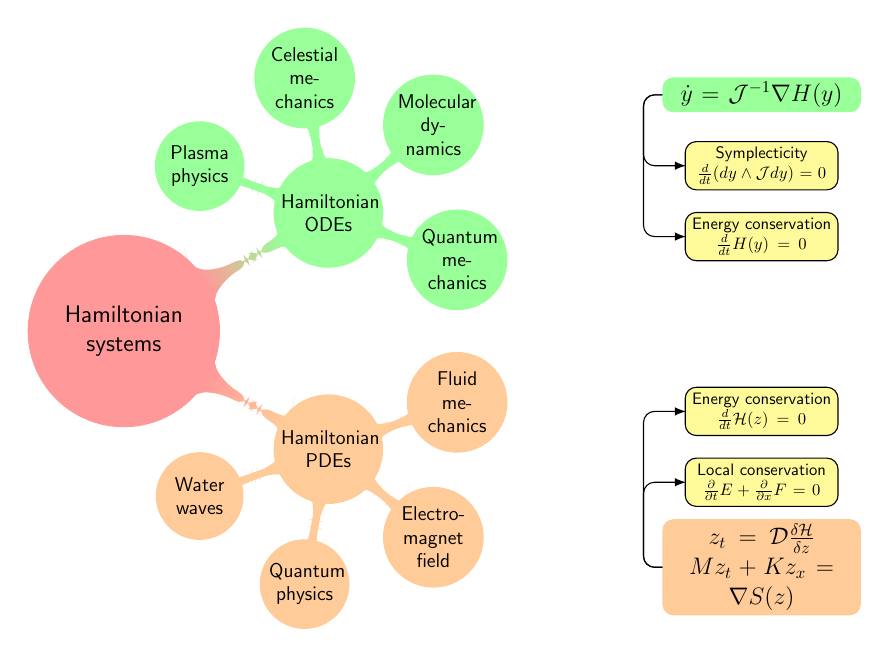
\begin{tikzpicture}[scale=0.6,transform shape,rounded corners,>=latex]
\centering
\path[mindmap,concept color=red!40,text=black]
      node[concept,font=\sf\Large]{Hamiltonian systems}
      [clockwise from=30]
      child[visible on=<2->,concept color=green!40] {
      node[concept,font=\sf \large]{Hamiltonian ODEs}
      [clockwise from=160]
      child{node[visible on=<2->,concept,font=\sf \large]{Plasma physics}}
      child{node[visible on=<2->,concept,font=\sf \large]{Celestial mechanics}}
      child{node[visible on=<2->,concept,font=\sf \large]{Molecular dynamics}}
      child{node[visible on=<2->,concept,font=\sf \large]{Quantum mechanics}}}  
      child[visible on=<3->,concept color=orange!40] {
      node[concept,font=\sf \large]{Hamiltonian PDEs}
      [clockwise from=20]
      child{node[visible on=<3->,concept,font=\sf \large] {Fluid mechanics}}
      child{node[visible on=<3->,concept,font=\sf \large] {Electro-\\magnet field}}
      child{node[visible on=<3->,concept, font=\sf \large] {Quantum physics}}
      child{node[visible on=<3->,concept,font=\sf \large] {Water waves}}};
\pause
\node[visible on=<4->,annotation,fill=green!40,text width=4cm,align=center,font=\sf \Large] at (13.5,5){$\dot{y}=\mathcal{J}^{-1}\nabla H(y)$};
\node[visible on=<5->,annotation,fill=orange!40,text width=4cm,align=center,font=\sf \Large] at (13.5,-5){$z_t=\mathcal{D}\frac{\delta\mathcal{H}}{\delta z}$\\$Mz_t+Kz_x=\nabla S(z)$};
\node[visible on=<6->,draw,fill=yellow!40,text width=3cm,align=center,font=\sf ] at (13.5,3.5){Symplecticity $\frac{d}{dt}(dy\wedge\mathcal{J}dy)=0$};  
\node[visible on=<7->,draw,fill=yellow!40,text width=3cm,align=center,font=\sf ] at (13.5,2){Energy conservation $\frac{d}{dt}H(y)=0$};     
\node[visible on=<8->, draw,fill=yellow!40,text width=3cm,align=center,font=\sf ] at (13.5,-3.2){Local conservation\\$\frac{\partial}{\partial t}E+\frac{\partial}{\partial x}F=0$};  
\node[visible on =<9->,draw,fill=yellow!40,text width=3cm,align=center,font=\sf ] at (13.5,-1.7){Energy conservation $\frac{d}{dt}\mathcal{H}(z)=0$};       
\draw[visible on=<6->, ->] (11.4,5)--(11,5)--(11,3.5)--(11.9,3.5);
\draw[visible on=<7->, ->] (11.4,5)--(11,5)--(11,2)--(11.9,2);
\draw[visible on=<8->, ->] (11.4,-5)--(11,-5)--(11,-3.2)--(11.9,-3.2);
\draw[visible on=<9->, ->] (11.4,-5)--(11,-5)--(11,-1.7)--(11.9,-1.7);
\end{tikzpicture}
\end{frame}

\begin{frame}
The canonical Hamiltonian system has the following form
\begin{equation}\label{eq-1}
\dot{p}=-H_q(p,q),\quad\dot{q}=H_p(p,q).
\end{equation}

Concerning numerical integration, the one-step method with time step $\tau$ defines the mapping
\begin{equation}\label{eq-2}
(p_{n+1},q_{n+1})=\Phi_\tau(p_n,q_n).
\end{equation}\\
\vspace{2mm}
The method \eqref{eq-2} is \textcolor{blue}{symplectic}, if
\begin{equation}\label{eq-3}
\left(\frac{\partial \Phi_\tau(p_n,q_n)}{\partial(p_n,q_n)}\right)^T\mathcal{J}\left(\frac{\partial \Phi_\tau(p_n,q_n)}{\partial(p_n,q_n)}\right)=\mathcal{J},
\end{equation}
where $\mathcal{J}=\left(\begin{array}{cc} 0 & \mathcal{I}\\ -\mathcal{I} & 0 \end{array}\right)$ and $\mathcal{I}$ is an identity matrix.\\
\vspace{2mm}
The method \eqref{eq-2} is \textcolor{blue}{energy-preserving}, if
\begin{equation}\label{eq-4}
H(p_{n+1},q_{n+1})=H(p_n,q_n).
\end{equation}
\end{frame}

\begin{frame}{Existing numerical methods}
Two prominent lines of investigation are currently the study of symplectic methods and energy-preserving methods.\\
\vspace{2mm}
\textcolor[rgb]{0,0,1}{$\blacktriangleright$} \textcolor{blue}{Symplectic methods:}\\
\quad\textcolor[rgb]{0,0,1}{$\bullet$} Generating function methods. Feng, 1984.\\
\quad\textcolor[rgb]{0,0,1}{$\bullet$} Symplectic Runge-Kutta methods. Sanz-Serna, 1988.\\
\quad\textcolor[rgb]{0,0,1}{$\bullet$} Composition methods. Yoshida, 1990, Qin, 1992.\\
\quad\textcolor[rgb]{0,0,1}{$\bullet$} Symplectic partitioned Runge-Kutta methods. Sun, 1993.\\
\quad\textcolor[rgb]{0,0,1}{$\bullet$} Variational integrators. Marsden, 1998. $\cdots$\\
\vspace{2mm}
\textcolor[rgb]{0,0,1}{$\blacktriangleright$} \textcolor{blue}{Energy-preserving methods:}\\
\quad\textcolor[rgb]{0,0,1}{$\bullet$} Projection methods. Hairer, Wanner, 1996.\\
\quad\textcolor[rgb]{0,0,1}{$\bullet$} Discrete gradient methods. Quispel, 1998.\\
\quad\textcolor[rgb]{0,0,1}{$\bullet$} Finite element methods. Betsch, Steinmann, 2000.\\
\quad\textcolor[rgb]{0,0,1}{$\bullet$} Averaged vector field methods. Quispel, McLaren, 2008.\\
\quad\textcolor[rgb]{0,0,1}{$\bullet$} Hamiltonian boundary value methods. Brugnano, 2010.\\
\quad\textcolor[rgb]{0,0,1}{$\bullet$} Partitioned averaged vector field methods. Cai, 2018.$\cdots$\\
\end{frame}	

\begin{frame}
There are currently many ways to construct symplectic methods, but of the methods obtained, only the following methods have the simplest form.\\
\vspace{4mm}
\textcolor[rgb]{0,0,1}{$\blacktriangleright$} \textcolor{blue}{Symplectic Euler methods:}
\begin{align}\label{eq-5}
\aligned
&p_{n+1}=p_n-\tau H_q(p_{n+1},q_n),\\
&q_{n+1}=q_n+\tau H_p(p_{n+1},q_n),\\
\endaligned
\quad\mbox{or}\quad
\aligned
&p_{n+1}=p_n-\tau H_q(p_n,q_{n+1}),\\
&q_{n+1}=q_n+\tau H_p(p_n,q_{n+1}).\\
\endaligned
\end{align}

\textcolor[rgb]{0,0,1}{$\blacktriangleright$} \textcolor{blue}{Implicit midpoint method:}
\begin{align}\label{eq-6}
\aligned
&p_{n+1}=p_n-\tau H_q\left(\frac{p_{n+1}+p_n}{2},\frac{q_{n+1}+q_n}{2}\right),\\
&q_{n+1}=q_n+\tau H_p\left(\frac{p_{n+1}+p_n}{2},\frac{q_{n+1}+q_n}{2}\right).\\
\endaligned
\end{align}	
\end{frame}	

\begin{frame}{Motivations}
It is natural to think about whether such a discretization scheme can be found to share both the symplecticity and energy conservation.\\	
\vspace{2mm}
\textcolor[rgb]{0,0,1}{$\blacktriangleright$} \textcolor{blue}{Symplectic \& energy-preserving~=~??}\\
\vspace{2mm}
\quad\textcolor[rgb]{0,0,1}{$\bullet$} Any symplectic Runge-Kutta method preserves the quadratic energy.\footnote{J.M. Sanz-Serna. {\em BIT}, 28:877--883, 1988.}\\
\vspace{2mm}
\quad\textcolor[rgb]{0,0,1}{$\bullet$} A constant time stepping algorithm is impossible to be at the same time symplectic and energy conserving.\footnote{Z. Ge and J.E. Marsden. {\em Phys. Lett. A}, 133:134--139, 1988.}\\
\vspace{2mm}
\quad\textcolor[rgb]{0,0,1}{$\bullet$} The only symplectic method that conserves the arbitrary Hamiltonian is the exact flow of the differential equation.\footnote{P. Chartier, E. Faou, and A. Murua. {\em Numer. Math.}, 103:575--590, 2006.}\\
\vspace{2mm}
\quad\textcolor[rgb]{0,0,1}{$\bullet$} Symplectic-energy-momentum integrators are obtained in a weaker sense by using time-adaptive steps.\footnote{C. Kane, J.E. Marsden, and M. Ortiz. {\em J. Math. Phys.}, 40:3353--3371, 1999.} \textcolor{blue}{(Low-order accuracy)}
\begin{equation*}
dp\wedge dq+\textcolor{blue}{dH\wedge dt}
\end{equation*}
\end{frame}	

\section{Two families of arbitrary high-order parameterized symplectic schemes}
\begin{frame}{A general symplectic scheme}
\textcolor[rgb]{0,0,1}{$\blacktriangleright$} \textcolor{blue}{Scheme I:}
\begin{align}\label{eq-7}
\aligned
&p_{n+1}=p_n-\tau H_q\big(\lambda p_{n+1}+(1-\lambda)p_n,\lambda q_n+(1-\lambda)q_{n+1}\big),\\
&q_{n+1}=q_n+\tau H_p\big(\lambda p_{n+1}+(1-\lambda)p_n,\lambda q_n+(1-\lambda)q_{n+1}\big),\\
\endaligned
\end{align}
where $\lambda$ is a real parameter.\\
\vspace{2mm}
\quad\textcolor[rgb]{0,0,1}{$\bullet$} When $\lambda=0$, $1$, $1/2$, the symplectic Euler methods and the implicit midpoint rule are covered. When $\lambda\neq 1/2$, Scheme I is a one-stage symplectic partitioned RK method. The Butcher tableau reads
\begin{equation}\label{eq-8}
\begin{tabular}{c|c}
$\lambda$ & $\lambda$\\ \hline
& $1$\
\end{tabular}\quad
\begin{tabular}{c|c}
$1-\lambda$ & $1-\lambda$\\ \hline
& $1$\\
\end{tabular}.
\end{equation}\\

\quad\textcolor[rgb]{0,0,1}{$\bullet$} Scheme I respresents a mapping $\Phi_\tau^{\lambda}: (p_n,q_n) \mapsto (p_{n+1},q_{n+1})$. The adjoint method of scheme I is
\begin{equation}\label{eq-9}
(\Phi_\tau^{\lambda})^*=\Phi_\tau^{1-\lambda}.
\end{equation}	

\begin{theorem}
Scheme I and its adjoint method are symplectic for any $\lambda$.
\end{theorem}
\end{frame}	

\begin{frame}
\quad\textcolor[rgb]{0,0,1}{$\bullet$} By fixing the parameter to specific values, we can obtain more symplectic schemes with simple forms that can be widely applied in practical computations.
\begin{subequations}\label{eq-10}
\begin{align}
\lambda=-1:&\left\{\aligned
&p_{n+1}=p_n-\tau H_q(2p_n-p_{n+1},2q_{n+1}-q_n),\\
&q_{n+1}=q_n+\tau H_p(2p_n-p_{n+1},2q_{n+1}-q_n);
\endaligned\right.\label{eq-10-a}\\
\lambda=\frac{1}{3}:&\left\{\aligned
&p_{n+1}=p_n-\tau H_q\left(\frac{2p_n+p_{n+1}}{3},\frac{2q_{n+1}+q_n}{3}\right),\\
&q_{n+1}=q_n+\tau H_p\left(\frac{2p_n+p_{n+1}}{3},\frac{2q_{n+1}+q_n}{3}\right);
\endaligned\right.\label{eq-10-b}\\ 
\lambda=\frac{3}{2}:&\left\{\aligned
&p_{n+1}=p_n-\tau H_q\left(\frac{3p_{n+1}-p_n}{2},\frac{3q_n-q_{n+1}}{2}\right),\\
&q_{n+1}=q_n+\tau H_p\left(\frac{3p_{n+1}-p_n}{2},\frac{3q_n-q_{n+1}}{2}\right);
\endaligned\right.\label{eq-10-c}\\
\lambda=2:&\left\{\aligned
&p_{n+1}=p_n-\tau H_q(2p_{n+1}-p_n,2q_n-q_{n+1}),\\
&q_{n+1}=q_n+\tau H_p(2p_{n+1}-p_n,2q_n-q_{n+1}).
\endaligned\right.\label{eq-10-d}
\end{align}
\end{subequations}	
\end{frame}	

\begin{frame}{Generating function with new coordinates}
We denote by $p,q \in\mathcal{R}^d$ the initial values $p_1,\cdots,p_d$ and $q_1,\cdots,q_d$ at $t_0$, respectively. Likewise, the solution of the system at $t_1$ are represented by $P,Q \in\mathcal{R}^d$. This implies that the mapping $(p,q) \mapsto (P,Q)$ is symplectic.

\begin{theorem}
Let $\lambda$ be a real number and the mapping $\varphi:(p,q) \mapsto (P,Q)$ be smooth, close to the identity. It is symplectic if and only if there exists locally a function $S(\lambda P+(1-\lambda)p,\lambda q+(1-\lambda)Q)$ such that
\begin{equation}\label{eq-11}
(Q-q)^Td\big(\lambda P+(1-\lambda)p\big)-(P-p)^Td\big(\lambda q+(1-\lambda)Q\big)=dS.
\end{equation}
\end{theorem}
	
Let the notations \textcolor{blue}{$u = \lambda P+(1-\lambda)p$, $v = \lambda q+(1-\lambda)Q$}, comparing the coefficients of $dS = \partial_uSdu+\partial_vSdv$ with the left side of \eqref{eq-11}, we derive the system
\begin{align}\label{eq-12}
\aligned
&P = p-\partial_vS\big(\lambda P+(1-\lambda)p,\lambda q+(1-\lambda)Q\big),\\
&Q = q+\partial_uS\big(\lambda P+(1-\lambda)p,\lambda q+(1-\lambda)Q\big).
\endaligned
\end{align}
\end{frame}

\begin{frame}
\begin{remark}
The above theorem gives a more general form of generating functions. When $\lambda = 0$, $1$, $1/2$, respectively, we reproduce the generating functions with the three typical coordinates\footnote{E. Hairer, C. Lubich, and G. Wanner. Springer-Verlag, Berlin, 2nd edition, 2006.} as follows:
\begin{itemize}
\item[\textcolor{black}{(1)}] $(Q-q)^Tdp-(P-p)^TdQ = dS_1(p,Q)$;
\item[\textcolor{black}{(2)}] $(Q-q)^TdP-(P-p)^Tdq = dS_2(P,q)$;
\item[\textcolor{black}{(3)}] $(Q-q)^Td(P+p)-(P-p)^Td(Q+q) = 2dS_3\left(\frac{P+p}{2},\frac{Q+q}{2}\right)$.
\end{itemize}
\end{remark}
\vspace{2mm}
\quad\textcolor[rgb]{0,0,1}{$\bullet$} In short, a generating function with new coordinates is introduced, which unifies the traditional three typical generating functions\footnote{K. Feng, H.M. Wu, M.Z. Qin, and D.L. Wang. {\em J. Comput. Math.}, 7:71--96, 1989.} that are widely used to construct symplectic schemes.\\
\vspace{2mm}
\quad\textcolor[rgb]{0,0,1}{$\bullet$} How to determine the generating function $S(u,v)$??\\
\end{frame}

\begin{frame}{The Hamilton-Jacobi equation with new variables}
Assuming the point $\big(P(t), Q(t)\big)$ to move in the exact flow of the system \eqref{eq-1}, it is found that a smooth generating function $S(u,v,t)$ generates via \eqref{eq-12} the exact flow of the Hamiltonian system.

\begin{theorem}
Let $\lambda$ be a real number. If $S(u,v,t)$ is a smooth solution of the partial differential equation
\begin{equation}\label{eq-13}
\frac{\partial S}{\partial t}(u,v,t)=H\big(u-(1-\lambda)\frac{\partial S}{\partial v}(u,v,t),v+\lambda\frac{\partial S}{\partial u}(u,v,t)\big)
\end{equation}
with initial condition $S(u,v,0) = 0$, then the mapping $(p,q) \mapsto (P,Q)$, defined by \eqref{eq-12}, is the exact flow of the Hamiltonian system \eqref{eq-1}.
\end{theorem}
	
\begin{remark}
When $\lambda = 0$, $1$, $1/2$, respectively, the Hamilton-Jacobi equations under the three typical variables\footnote{E. Hairer, C. Lubich, and G. Wanner. Springer-Verlag, Berlin, 2nd edition, 2006.} are obtained.
\end{remark}
\end{frame}

\begin{frame}{Parameterized generating function methods\footnote{Y.H. Bo, W.J. Cai, and Y.S. Wang. {\em Adv. Appl. Math. Mech.}, 13:982-1004, 2021.}}
An approximate solution of the Hamilton-Jacobi equation \eqref{eq-13} can construct symplectic schemes of any order. For this purpose, we consider a convergent power series in $t$ as follows:
\begin{equation}\label{eq-14}
S(u,v,t)=\sum_{i=1}^{\infty} K_i(u,v)t^i.
\end{equation}
Inserting this series into \eqref{eq-13} and comparing like powers of $t$, this follows
\begin{subequations}\label{eq-15}
\begin{align}
&K_1(u,v)=H(u,v),\label{eq-15-a}\\
&K_2(u,v)=(\lambda-\frac{1}{2})\left((\frac{\partial H}{\partial u})^T\frac{\partial H}{\partial v}\right)(u,v),\label{eq-15-b}\\
&K_3(u,v)=\frac{1}{2}(\lambda^2-\lambda+\frac{1}{3})\left((\frac{\partial H}{\partial u})^T \frac{\partial^2H}{\partial v^2}\frac{\partial H}{\partial u}+(\frac{\partial H}{\partial v})^T \frac{\partial^2H}{\partial u^2}\frac{\partial H}{\partial v}\right)(u,v)
\nonumber\\&\quad\quad\quad\quad~~+(\lambda^2-\lambda+\frac{1}{6})\left((\frac{\partial H}{\partial v})^T\frac{\partial^2H}{\partial u\partial v}\frac{\partial H}{\partial u}\right)(u,v).\label{eq-15-c}
\end{align}
\end{subequations}
\end{frame}

\begin{frame}
A natural way to approximate $S$ is take the truncation of \eqref{eq-14}. More precisely, we replace \eqref{eq-14} with the truncated series
\begin{equation}\label{eq-16}
\bar{S}(u,v)=\sum_{i=1}^{r} K_i(u,v)\tau^i.
\end{equation}
Then we get a symplectic scheme of order $r$.\\
\vspace{2mm}
\textcolor[rgb]{0,0,1}{$\blacktriangleright$} \textcolor{blue}{Scheme I:}
\begin{align}\label{eq-17}
\aligned
&p_{n+1}=p_n-\tau\partial_{\bar{v}}H(\bar{u},\bar{v}),\\
&q_{n+1}=q_n+\tau\partial_{\bar{u}}H(\bar{u},\bar{v}).\\
\endaligned
\end{align}\\

\textcolor[rgb]{0,0,1}{$\blacktriangleright$} \textcolor{blue}{Scheme II:}
\begin{align}\label{eq-18}
\aligned
&p_{n+1}=p_n-\tau\partial_{\bar{v}}H(\bar{u},\bar{v})-(\lambda-\frac{1}{2})\tau^2\left(\frac{\partial^2H}{\partial {\bar{v}}^2}\frac{\partial H}{\partial {\bar{u}}}+\frac{\partial^2H}{\partial {\bar{v}}\partial {\bar{u}}}\frac{\partial H}{\partial {\bar{v}}}\right)(\bar{u},\bar{v}),\\
&q_{n+1}=q_n+\tau\partial_{\bar{u}}H(\bar{u},\bar{v})+(\lambda-\frac{1}{2})\tau^2\left(\frac{\partial^2H}{\partial {\bar{u}}^2}\frac{\partial H}{\partial {\bar{v}}}+\frac{\partial^2H}{\partial {\bar{u}}\partial {\bar{v}}}\frac{\partial H}{\partial {\bar{u}}}\right)(\bar{u},\bar{v}).\\
\endaligned
\end{align}
The notations \textcolor{blue}{$\bar{u} = \lambda p_{n+1}+(1-\lambda)p_n,\ \bar{v} = \lambda q_n+(1-\lambda)q_{n+1}$} are used.
\end{frame}

\begin{frame}{Symmetric composition methods}
We consider the symmetric composition method\footnote{H.~Yoshida. {\em Phys. Lett. A}, 150:262--268, 1990.} of Scheme I and get the following symmetric symplectic scheme of order $2$.\\
\vspace{3mm}
\textcolor[rgb]{0,0,1}{$\blacktriangleright$} \textcolor{blue}{Scheme III:}
\begin{equation}\label{eq-19}
\Psi_\tau\triangleq \Phi_{\frac{\tau}{2}}^{\lambda} \circ (\Phi_{\frac{\tau}{2}}^{\lambda})^*=\Phi_{\frac{\tau}{2}}^{\lambda} \circ \Phi_{\frac{\tau}{2}}^{1-\lambda}: (p_n,q_n) \mapsto (p_{n+1},q_{n+1}).
\end{equation}\\
\vspace{3mm}
\quad\textcolor[rgb]{0,0,1}{$\bullet$} The symplecticity of Scheme III follows from the fact that the composition of symplectic schemes is still symplectic.\\ 
\vspace{3mm}
\quad\textcolor[rgb]{0,0,1}{$\bullet$} Using the idea of composition methods\footnote{M.Z. Qin and W.J. Zhu. {\em Computing}, 47:309--321, 1992.}, this procedure can also be repeated all the time to construct the higher order symmetric symplectic scheme without higher derivatives.
\end{frame}

\begin{frame}{Multi-parametric symplectic schemes\footnote{Y.H. Bo, W.J. Cai, and Y.S. Wang. {\em Appl. Math. Lett.}, 112:106792, 2021.}}
\textcolor[rgb]{0,0,1}{$\blacktriangleright$} \textcolor{blue}{Three-parameter symplectic scheme:}
\begin{equation}\label{eq-20}
\begin{tabular}{c|c}
$\alpha$ & $\gamma\alpha$\quad $(1-\gamma)\alpha$\\ 
$\beta$ & $\gamma\beta$\quad $(1-\gamma)\beta$\\ \hline
& $\gamma$\quad\quad\ $1-\gamma$\\
\end{tabular}\quad
\begin{tabular}{c|c}
$(1-\beta)+\gamma(1-\alpha)$ & $(1-\alpha)\gamma$\quad $(1-\beta)(1-\gamma)$\\ 
$(1-\beta)+\gamma(1-\alpha)$ & $(1-\alpha)\gamma$\quad $(1-\beta)(1-\gamma)$\\ \hline
& $\gamma$\quad\quad\quad\quad$1-\gamma$\\
\end{tabular}
\end{equation}
with three free parameters $\alpha$, $\beta$ and $\gamma$.\\
\vspace{2mm}
\quad\textcolor[rgb]{0,0,1}{$\bullet$} The scheme \eqref{eq-20} is symplectic. When the relation $\gamma=(1/2-\beta)/(\alpha-\beta)$ is satisfied with $\alpha<\beta$, it is of order $2$.\\
\vspace{2mm}
\textcolor[rgb]{0,0,1}{$\blacktriangleright$} \textcolor{blue}{One-parameter symplectic scheme:}
\begin{equation}\label{eq-21}
\begin{tabular}{c|c}
$\alpha$ & $\frac{1}{2}\alpha$\quad\quad\quad\  $\frac{1}{2}\alpha$\\ 
$1-\alpha$ & $\frac{1}{2}(1-\alpha)$\quad $\frac{1}{2}(1-\alpha)$\\ \hline
& $\frac{1}{2}$\quad\quad\quad\quad $\frac{1}{2}$\\
\end{tabular}\quad\quad
\begin{tabular}{c|c c}
$\frac{1}{2}$ & $\frac{1}{2}(1-\alpha)$\quad $\frac{1}{2}\alpha$\\ 
$\frac{1}{2}$ & $\frac{1}{2}(1-\alpha)$\quad $\frac{1}{2}\alpha$\\ \hline
&~~~~$\frac{1}{2}$\quad\quad\quad$\frac{1}{2}$\\
\end{tabular}.
\end{equation}
\quad\textcolor[rgb]{0,0,1}{$\bullet$} The scheme \eqref{eq-21} is a second-order symmetric symplectic scheme with a free parameter and generalizes the St\"{o}rmer-Verlet method ($\alpha=0$).
\end{frame}

\begin{frame}{Concluding remarks}
\quad\textcolor[rgb]{0,0,1}{$\bullet$} A general parametric symplectic scheme covers the symplectic Euler methods and the midpoint rule. By fixing the parameter to specific values, we can obtain more symplectic schemes with simple forms that can be widely applied in practical computations.\\  
\vspace{4mm}
\quad\textcolor[rgb]{0,0,1}{$\bullet$} A more general form of generating functions and the Hamilton-Jacobi equations is proposed, which generalizes the three typical ones widely used to construct symplectic algorithms.\\
\vspace{4mm}
\quad\textcolor[rgb]{0,0,1}{$\bullet$} Two classes of arbitrary high-order parameterized symplectic schemes enrich the types of available symplectic methods.\\
\vspace{4mm}
\quad\textcolor[rgb]{0,0,1}{$\bullet$} Some multi-parametric symplectic schemes are also given, which have more freedom to design integrators which preserve several non-quadratic invariants.\\
\end{frame}

\begin{frame}{Numerical experiments: the H\'{e}non-Heiles model}
The H\'{e}non-Heiles model originates from a problem in celestial mechanics. The dynamics is described by a Hamiltonian of the form
\begin{equation*}
H(p_1,p_2,q_1,q_2)=\frac{1}{2}(p_1^2+p_2^2)+U(q_1,q_2).
\end{equation*}
The following potential $U$ is chosen as
\begin{equation*}
U(q_1,q_2)=\frac{1}{2}(q_1^2+q_2^2+2 q_1^2 q_2-\frac{2}{3}q_2^3).
\end{equation*}
The two classical orbits will be illustrated with the initial value as follows:\\ 
\begin{itemize}
\item Box orbit: $H_0=0.02,\ p_2(0)=0,\ q_1(0)=0,\ q_2(0)=-0.082$;
\item Chaotic orbit: $H_0=1/6,\ p_2(0)=0,\ q_1(0)=0,\ q_2(0)=0.82$.
\end{itemize}
The values of $p_1(0)$ are found from the Hamiltonian.
\end{frame}

\begin{frame}{Box orbits of Scheme I}
\begin{figure}
\centering
\subfigure[$\lambda=-1$]{
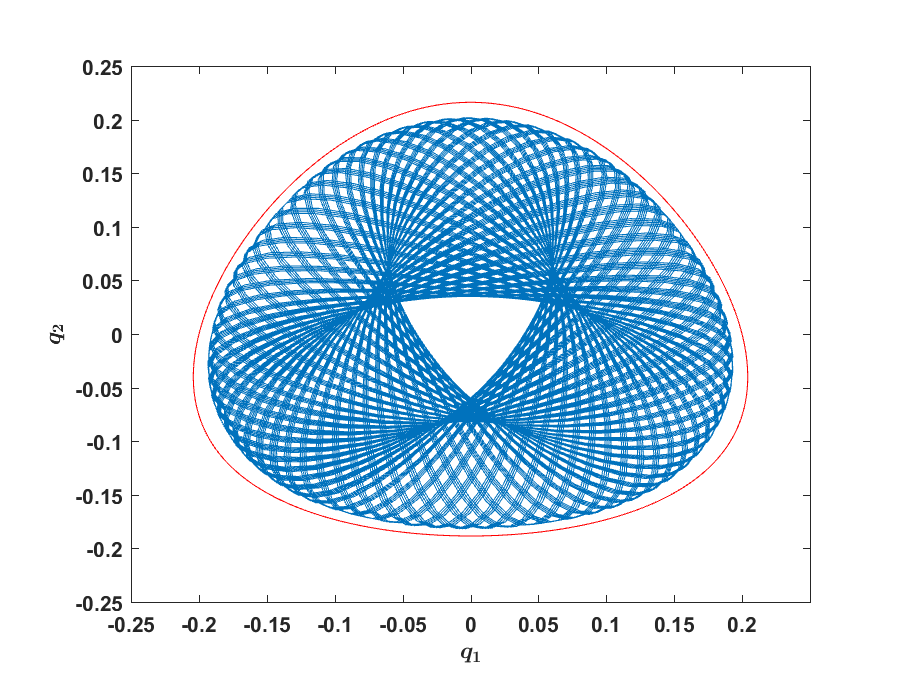
\includegraphics[width=42mm]{1_bHH_sym_R}}\vspace{-1mm}
\subfigure[$\lambda=\frac{1}{3}$]{
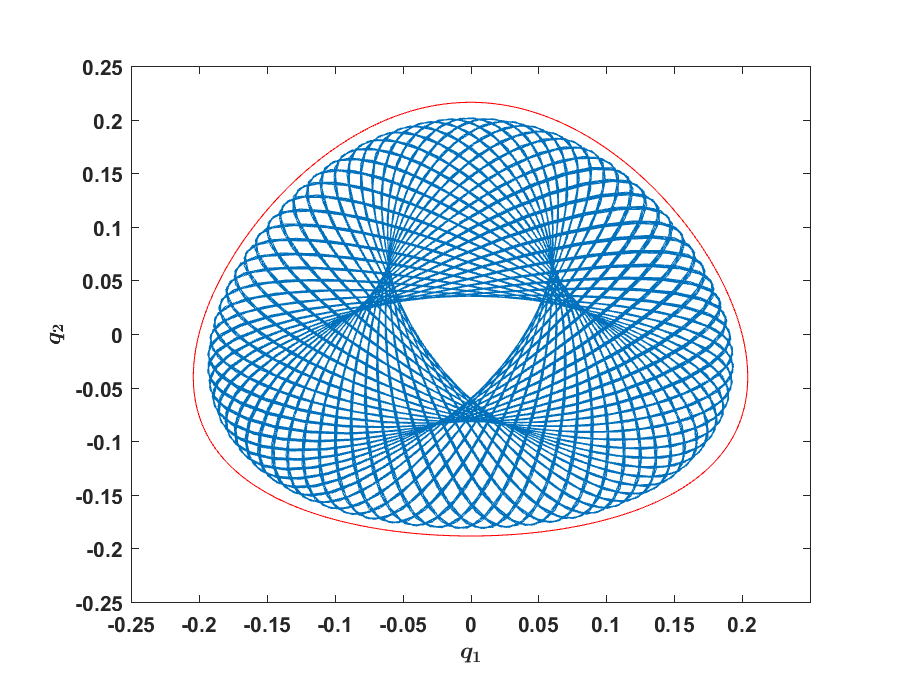
\includegraphics[width=42mm]{13_bHH_sym_R}}\vspace{-1mm}
\subfigure[$\lambda=\frac{3}{2}$]{
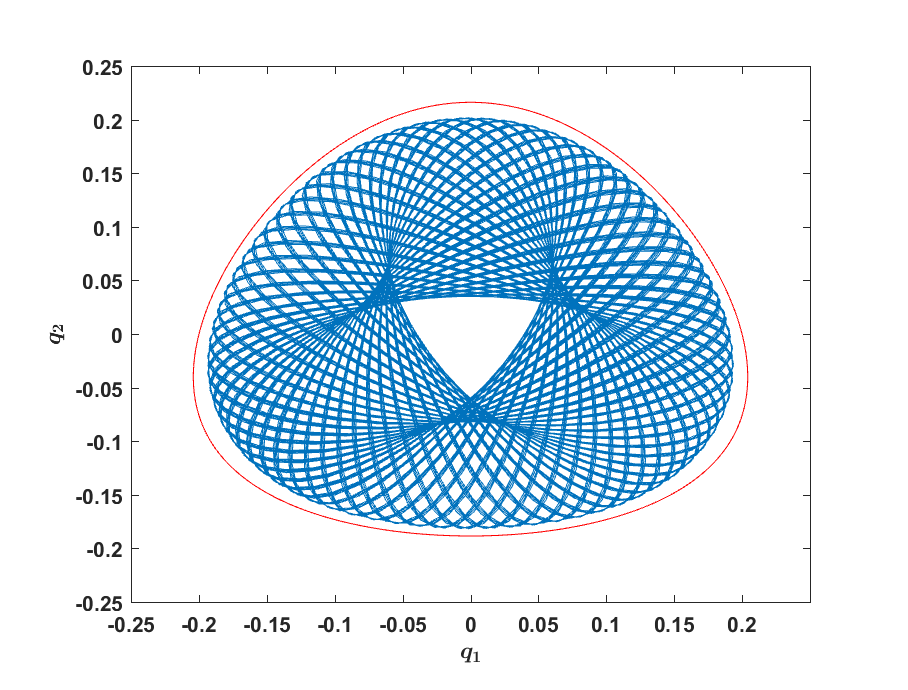
\includegraphics[width=42mm]{32_bHH_sym_R}}
\subfigure[$\lambda=2$]{
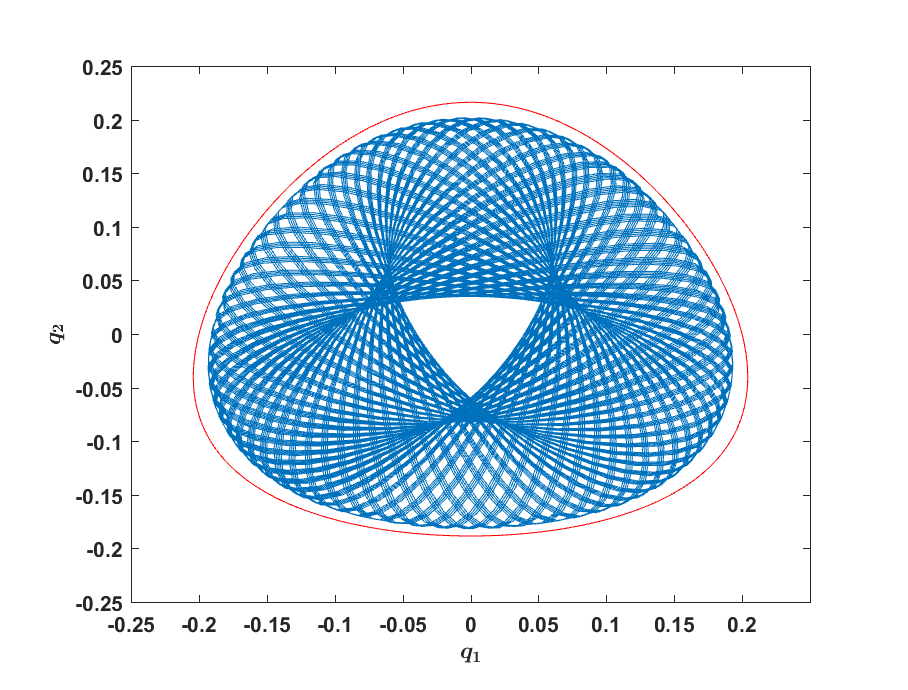
\includegraphics[width=42mm]{2_bHH_sym_R}}
\end{figure}
\end{frame}

\begin{frame}{Chaotic orbits of Scheme I}
\begin{figure}
\centering
\subfigure[$\lambda=-1$]{
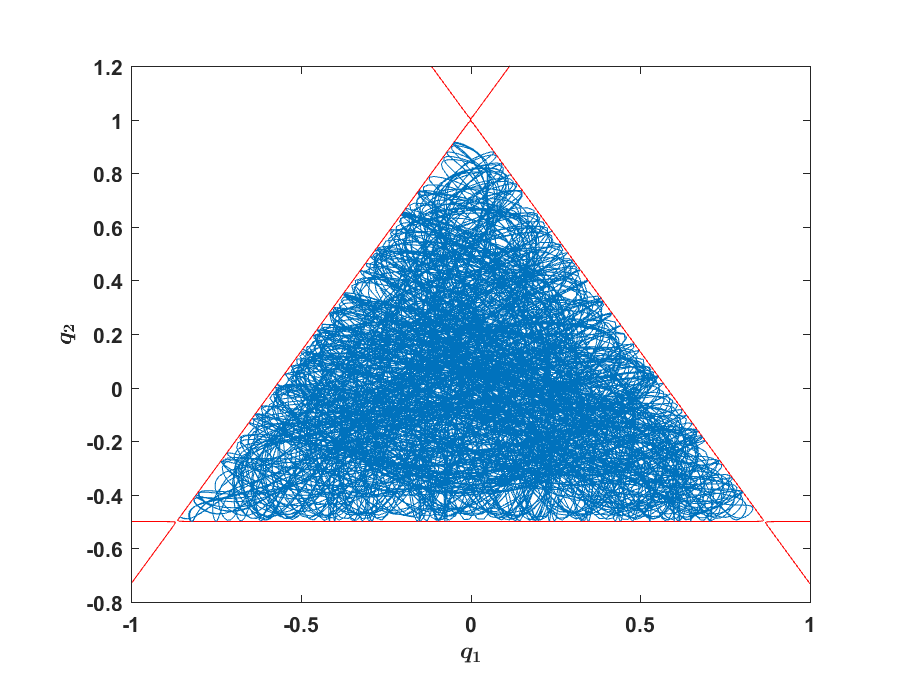
\includegraphics[width=42mm]{1_cHH_sym_R}}\vspace{-1mm}
\subfigure[$\lambda=\frac{1}{3}$]{
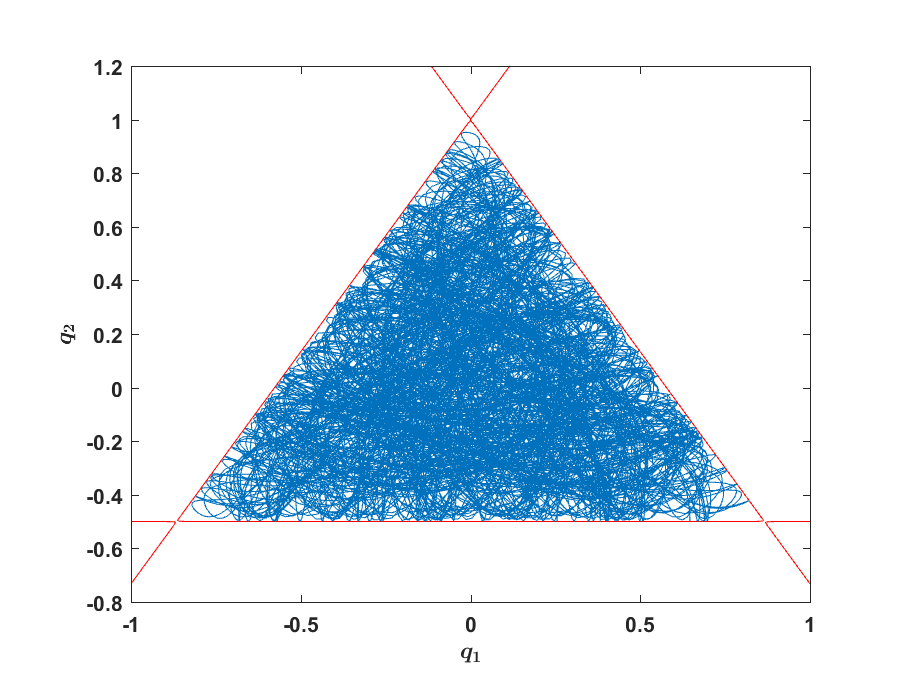
\includegraphics[width=41mm]{13_cHH_sym_R}}\vspace{-1mm}
\subfigure[$\lambda=\frac{3}{2}$]{
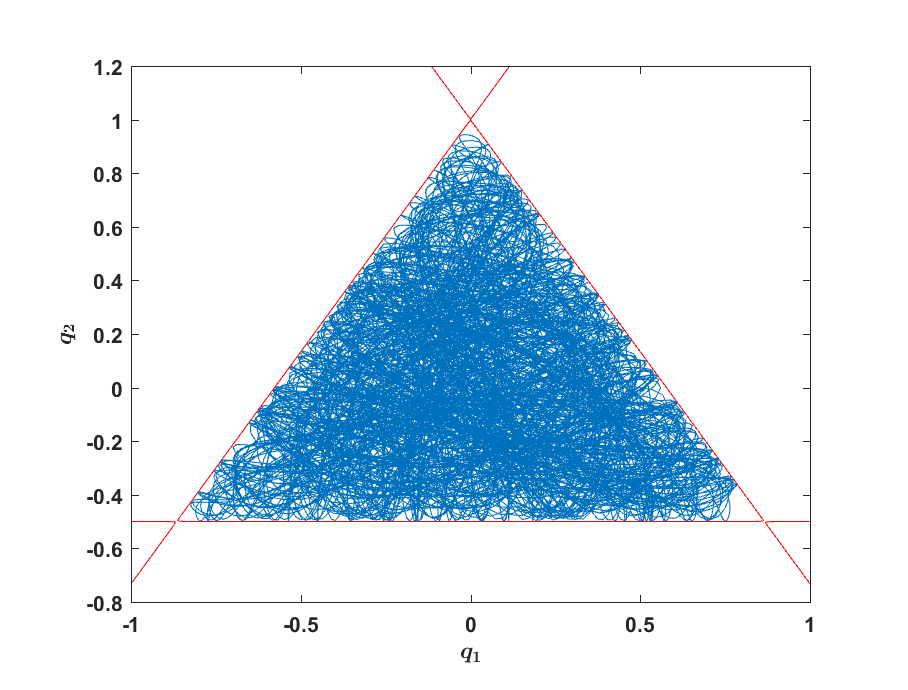
\includegraphics[width=42mm]{32_cHH_sym_R}}
\subfigure[$\lambda=2$]{
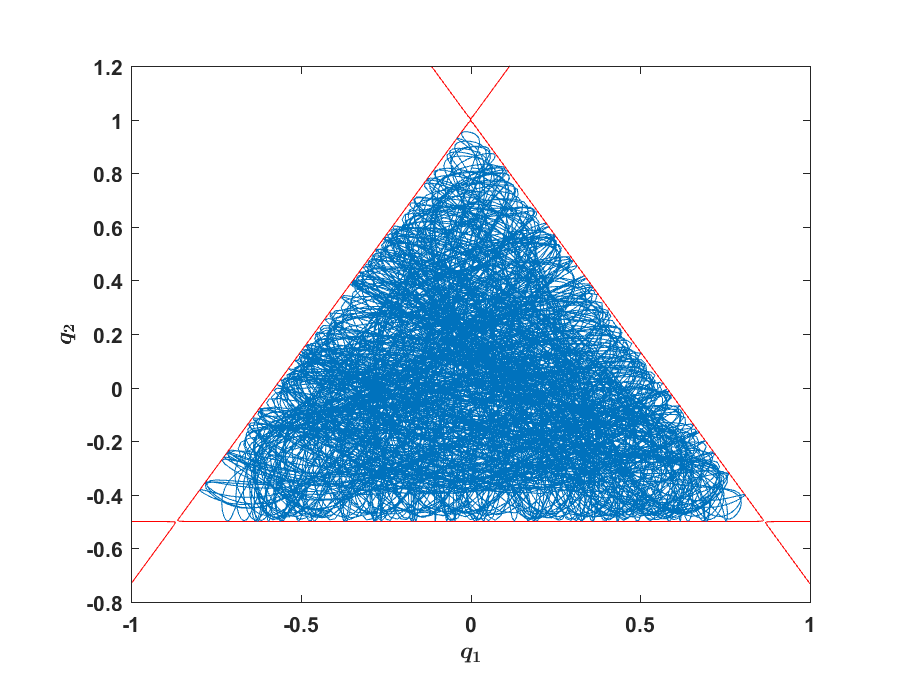
\includegraphics[width=42mm]{2_cHH_sym_R}}
\end{figure}
\end{frame}

\begin{frame}{Energy errors of box (first row) and chaotic orbits}
\begin{figure}
\centering
\subfigure[Scheme I (left)]{
\begin{minipage}[t]{0.33\textwidth}
\centering
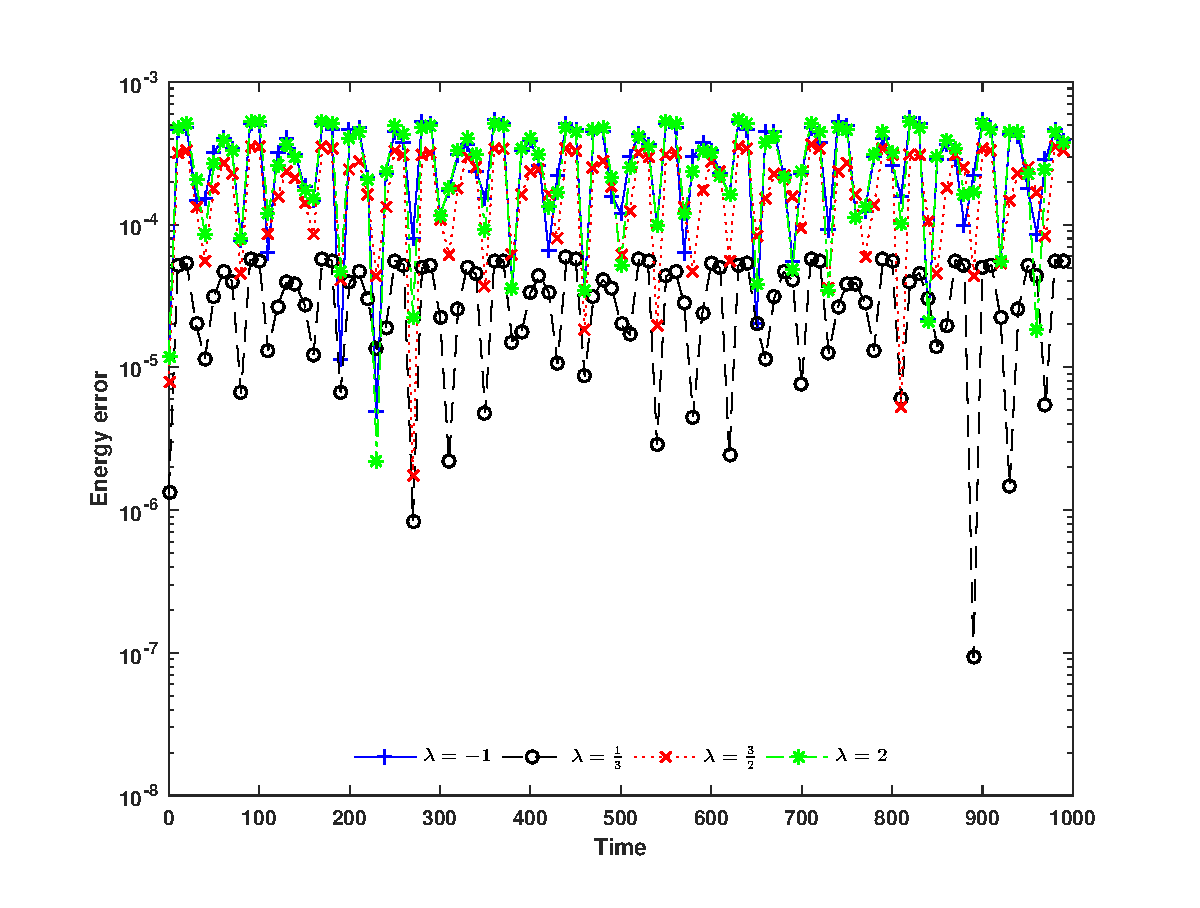
\includegraphics[width=42mm]{bHH_sym_HE}\\
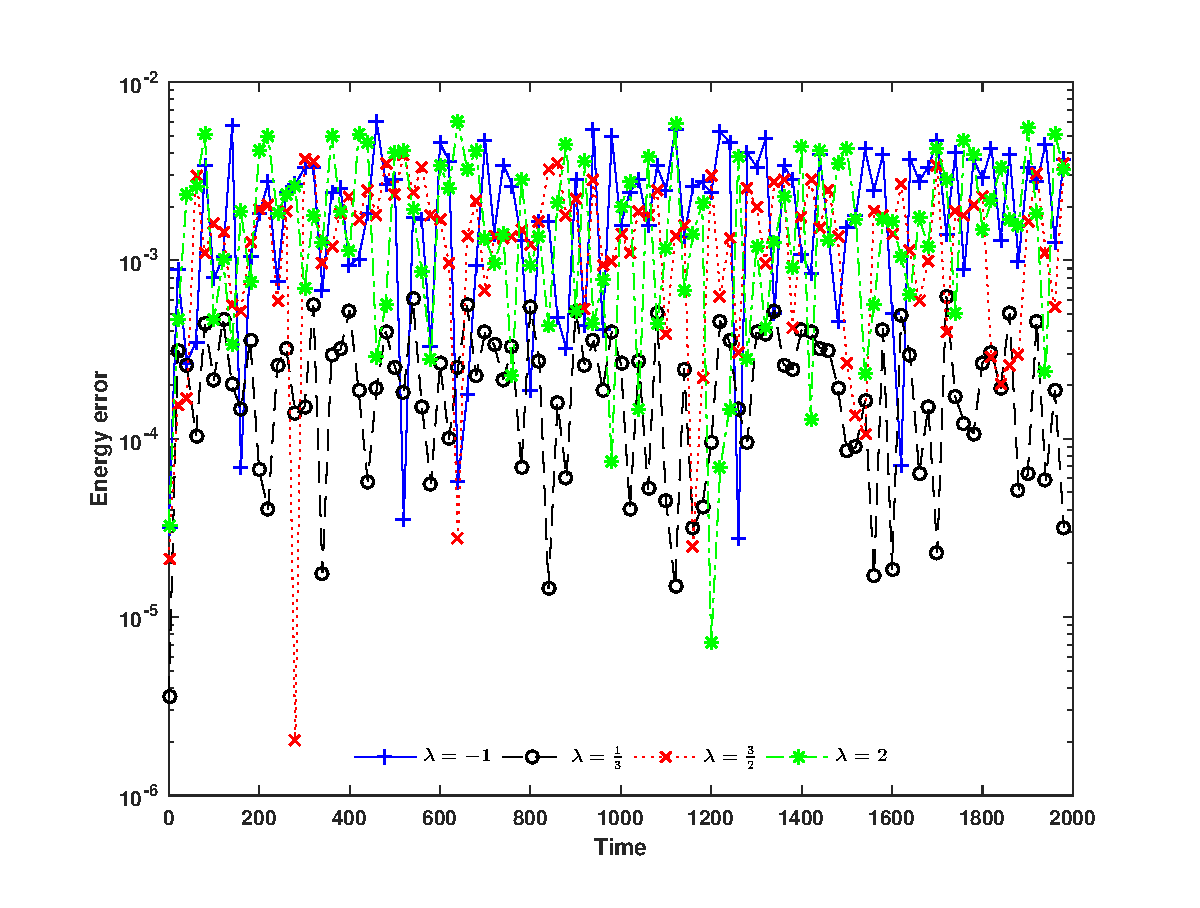
\includegraphics[width=42mm]{cHH_sym_HE}
\end{minipage}}\hspace{-3mm}
\subfigure[Scheme II (middle)]{
\begin{minipage}[t]{0.33\textwidth}
\centering
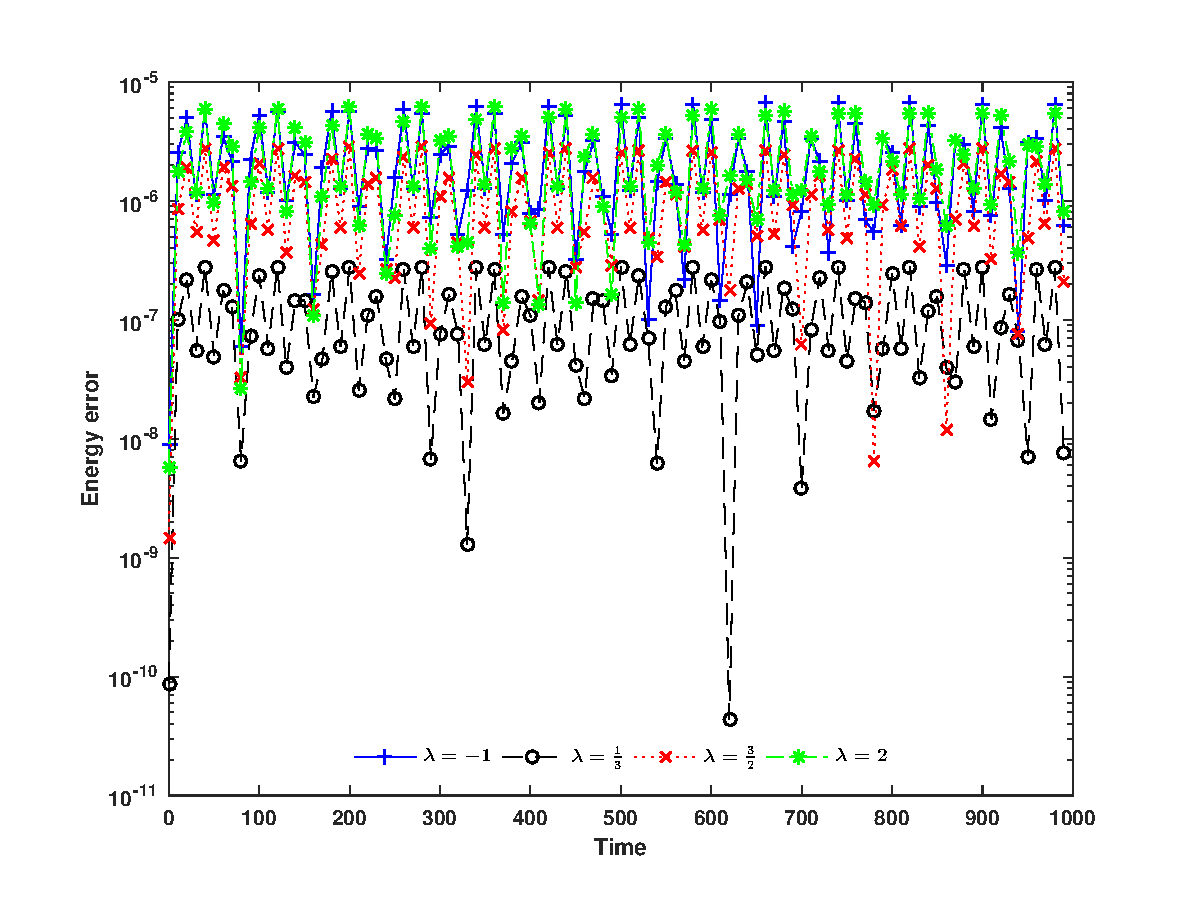
\includegraphics[width=42mm]{bHH_K2_sym_HE}\\
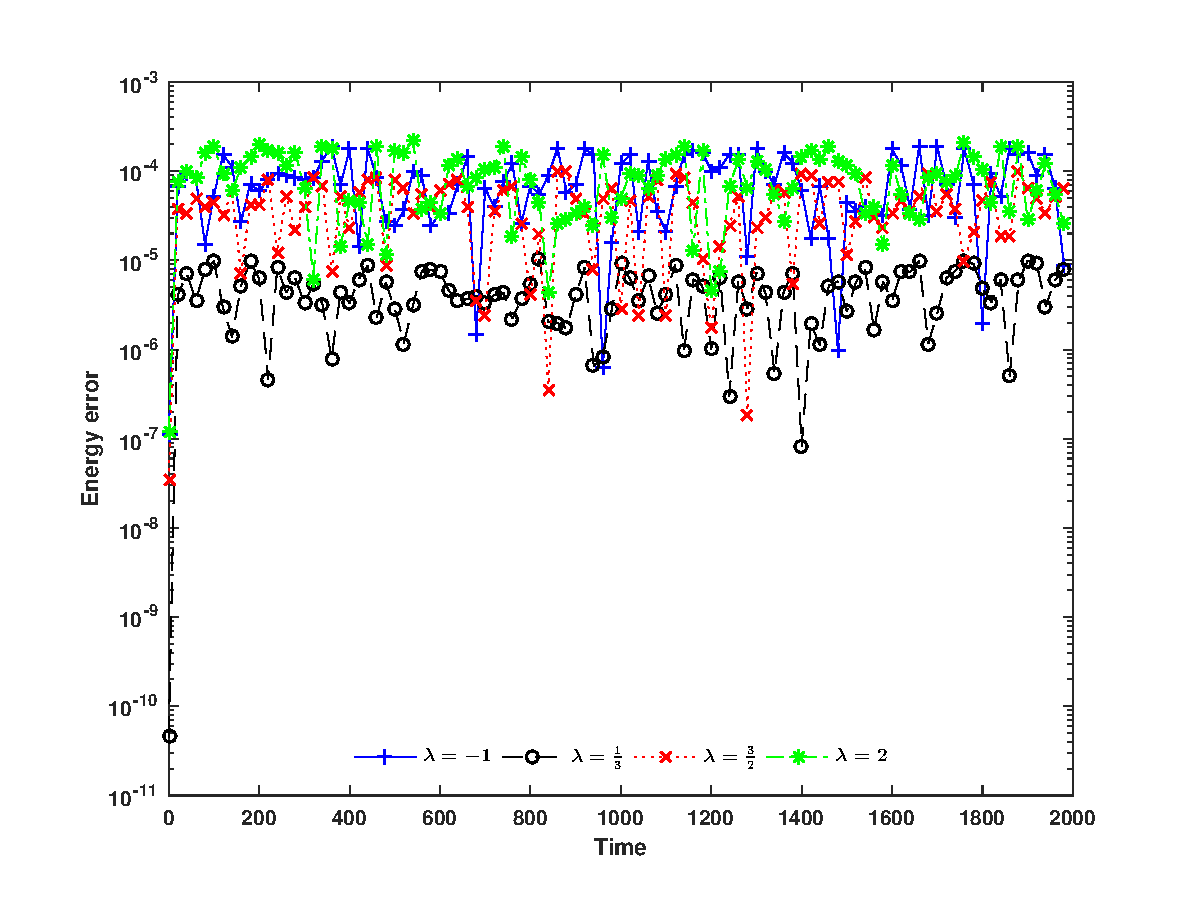
\includegraphics[width=42mm]{cHH_K2_sym_HE}
\end{minipage}}\hspace{-3mm}
\subfigure[Scheme III (right)]{
\begin{minipage}[t]{0.33\textwidth}
\centering
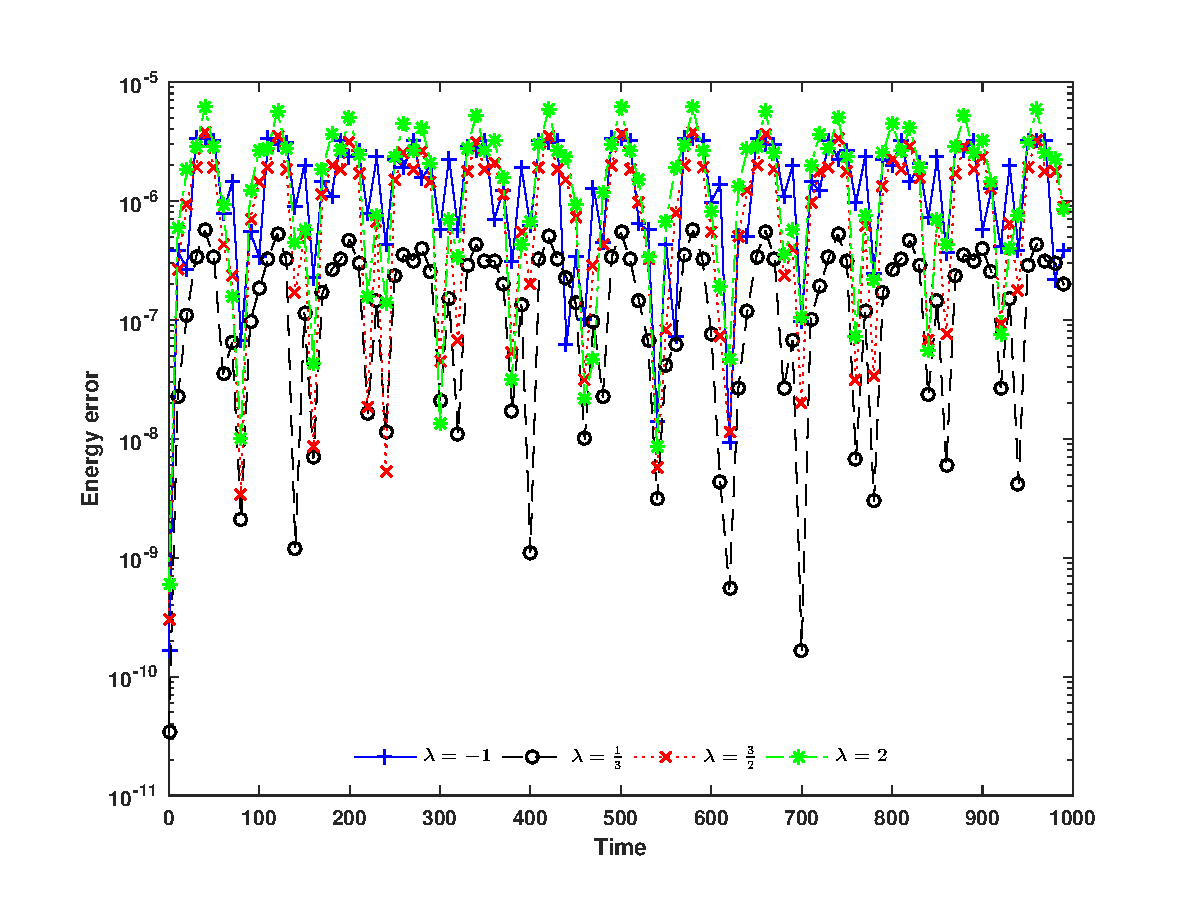
\includegraphics[width=42mm]{bHH2_sym_HE}\\
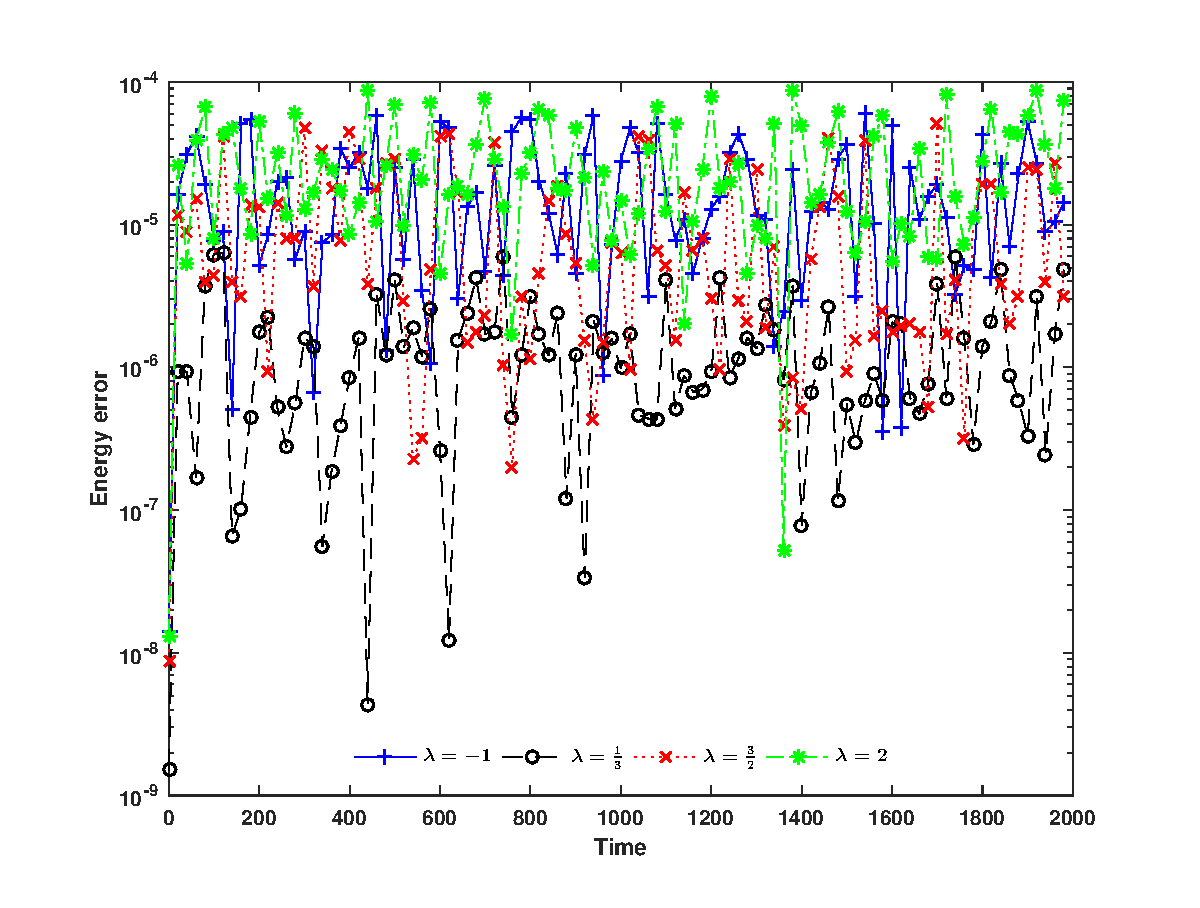
\includegraphics[width=42mm]{cHH2_sym_HE}
\end{minipage}}
\end{figure}
\end{frame}

\begin{frame}{Convergence tests with chaotic orbits at $t=1$}
\begin{table}
\tabcolsep=3pt \small \renewcommand \arraystretch{1.2} \centering
\begin{tabularx}{\textwidth}{*{10}{l}} \toprule
\multirow{2}*{Scheme} & \multirow{2}*{$\tau$} & \multicolumn{2}{c}{$\lambda=-1$} & \multicolumn{2}{c}{$\lambda=\frac{1}{3}$} & \multicolumn{2}{c}{$\lambda=\frac{3}{2}$} & \multicolumn{2}{c}{$\lambda=2$}\\
\cmidrule(lr){3-4}\cmidrule(lr){5-6}\cmidrule(lr){7-8}\cmidrule(lr){9-10}
&& Error & Order & Error & Order & Error & Order & Error & Order\\ \midrule
\multirow{4}*{I}
& 0.02/2 & 4.31E-03 & - & 4.38E-04 & - & 2.63E-03 & - & 3.85E-03 & -\\
& 0.02/4 & 2.09E-03 & 1.04 & 2.23E-04 & 0.98 & 1.34E-03 & 0.98 & 1.98E-03 & 0.96\\
& 0.02/8 & 1.03E-03 & 1.02 & 1.12E-04 & 0.99 & 6.73E-04 & 0.99 & 1.00E-03 & 0.98\\
& 0.02/16 & 5.13E-04 & 1.01 & 5.63E-05 & 0.99 & 3.38E-04 & 0.99 & 5.06E-04 & 0.99\\ \bottomrule
\multirow{4}*{II}
& 0.02/2 & 5.09E-04 & - & 2.35E-05 & - & 2.24E-04 & - & 4.77E-04 & -\\
& 0.02/4 & 1.25E-04 & 2.02 & 5.87E-06 & 2.00 & 5.67E-05 & 1.98 & 1.21E-04 & 1.98\\
& 0.02/8 & 3.11E-05 & 2.01 & 1.47E-06 & 2.00 & 1.42E-05 & 1.99 & 3.06E-05 & 1.99\\
& 0.02/16 & 7.74E-06 & 2.01 & 3.67E-07 & 2.00 & 3.57E-06 & 2.00 & 7.68E-06 & 1.99\\ \bottomrule
\multirow{4}*{III}
& 0.02/2 & 1.12E-04 & - & 3.54E-06 & - & 5.04E-05 & - & 1.18E-04 & -\\
& 0.02/4 & 2.79E-05 & 2.00 & 8.84E-07 & 2.00 & 1.26E-05 & 2.00 & 2.94E-05 & 2.00\\
& 0.02/8 & 6.97E-06 & 2.00 & 2.21E-07 & 2.00 & 3.15E-06 & 2.00 & 7.34E-06 & 2.00\\
& 0.02/16 & 1.74E-06 & 2.00 & 5.52E-08 & 2.00 & 7.88E-07 & 2.00 & 1.84E-06 & 2.00\\ \bottomrule
\end{tabularx}
\end{table}
\end{frame}

\begin{frame}{Numerical experiments: the perturbed Kepler problem}
Our second experiment is the motion of a planet in the Schwarzschild potential for Einstein's general relativity theory. The Hamiltonian of the dynamics reads
\begin{equation*}
H(p_1,p_2,q_1,q_2)=\frac{1}{2}(p_1^2+p_2^2)-\frac{1}{\sqrt{q_1^2+q_2^2}}-\frac{\mu}{3\sqrt{(q_1^2+q_2^2)^3}},
\end{equation*}
where $\mu$ is a positive or negative small number. Moreover, the angular momentum of this system
\begin{equation*}
L(p_1,p_2,q_1,q_2)=q_1p_2-q_2p_1
\end{equation*}
is a quadratic first integral. We choose the initial points as
\[p_1(0)=0,\ p_2(0)=\sqrt{\frac{1+e}{1-e}},\ q_1(0)=1-e,\ q_2(0)=0,\]
which confers an eccentricity $e$ on the orbit. We set $e=0.6$ and $\mu=0.0075$ in this experiment. Then $H(p,q)=H_0\approx-0.5391$, $L(p,q)=L_0=0.8$. The system represents approximately an ellipse orbit for $H_0<0$.
\end{frame}

\begin{frame}{Numerical orbits of Scheme I}
\begin{figure}
\centering
\subfigure[$\lambda=-1$]{
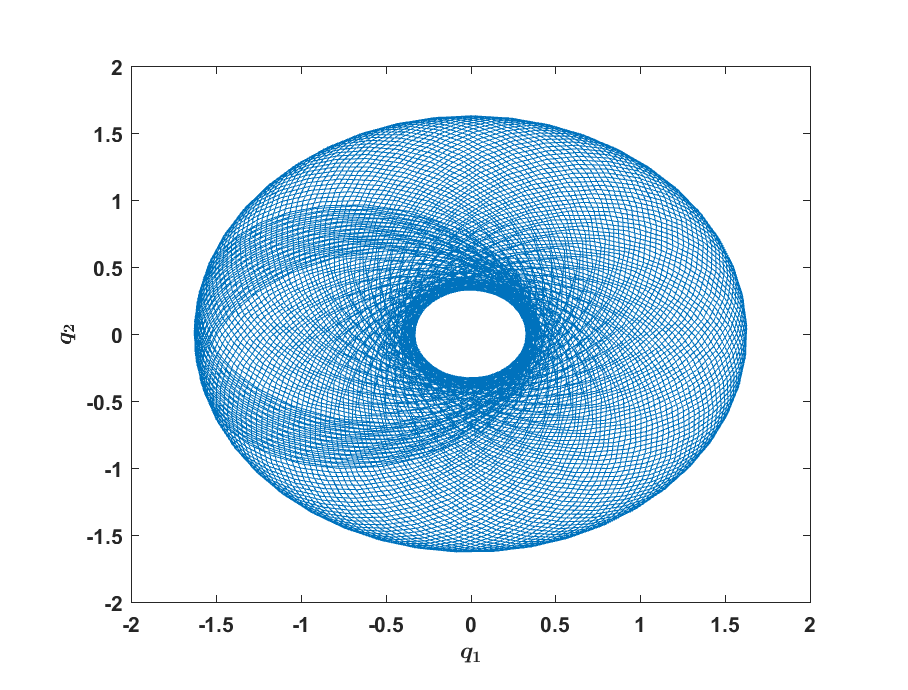
\includegraphics[width=42mm]{1_perKepler_sym_R}}\vspace{-1mm}
\subfigure[$\lambda=\frac{1}{3}$]{
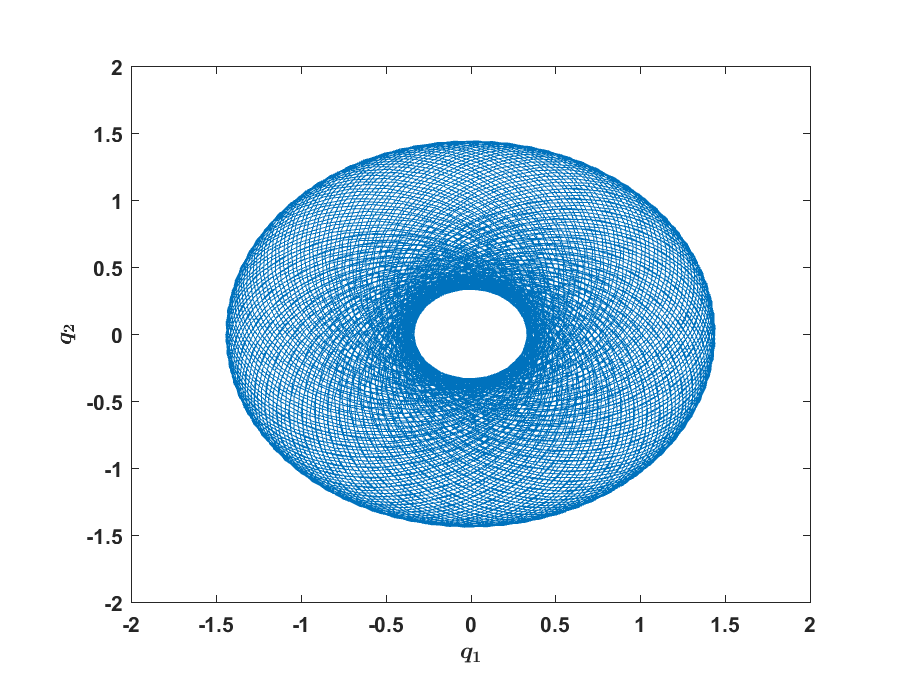
\includegraphics[width=42mm]{13_perKepler_sym_R}}\vspace{-1mm}
\subfigure[$\lambda=\frac{3}{2}$]{
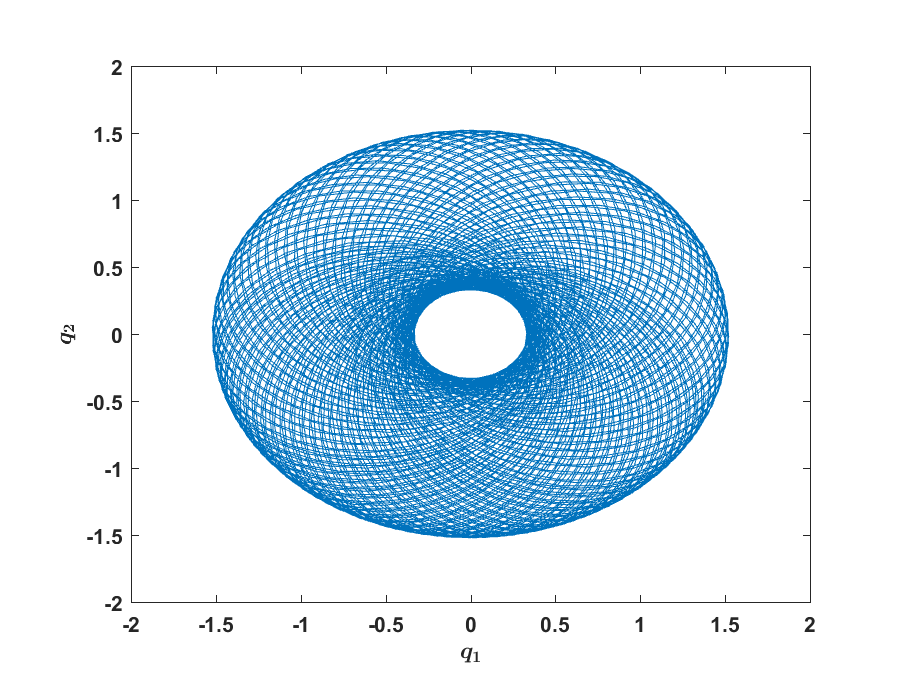
\includegraphics[width=42mm]{32_perKepler_sym_R}}
\subfigure[$\lambda=2$]{
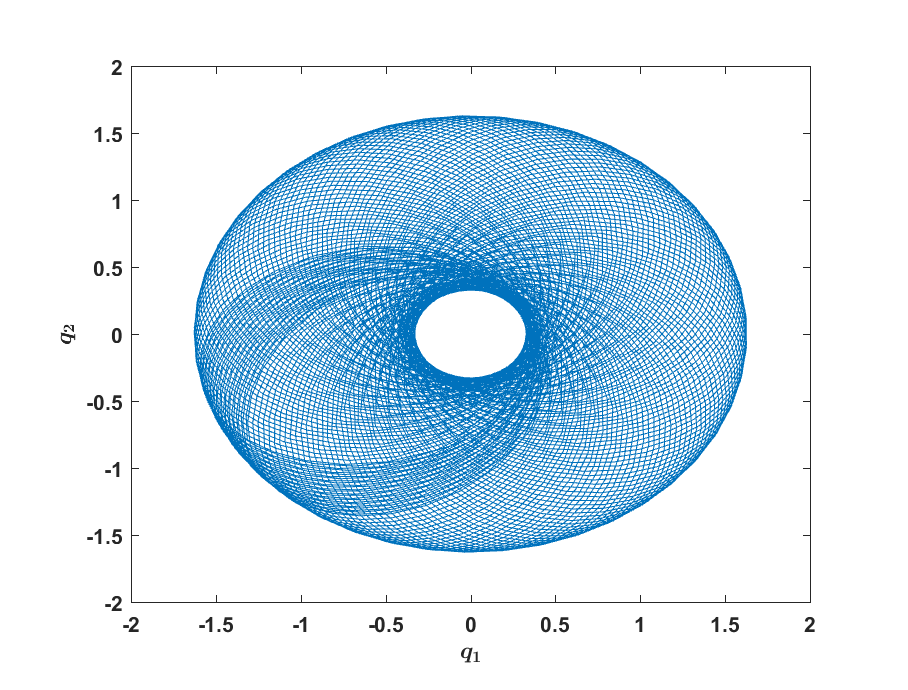
\includegraphics[width=42mm]{2_perKepler_sym_R}}
\end{figure}
\end{frame}

\begin{frame}{Energy and angular momentum errors of Schemes I and III}
\begin{figure}
\centering
\subfigure[Scheme I (left)]{
\begin{minipage}[t]{0.33\textwidth}
\centering
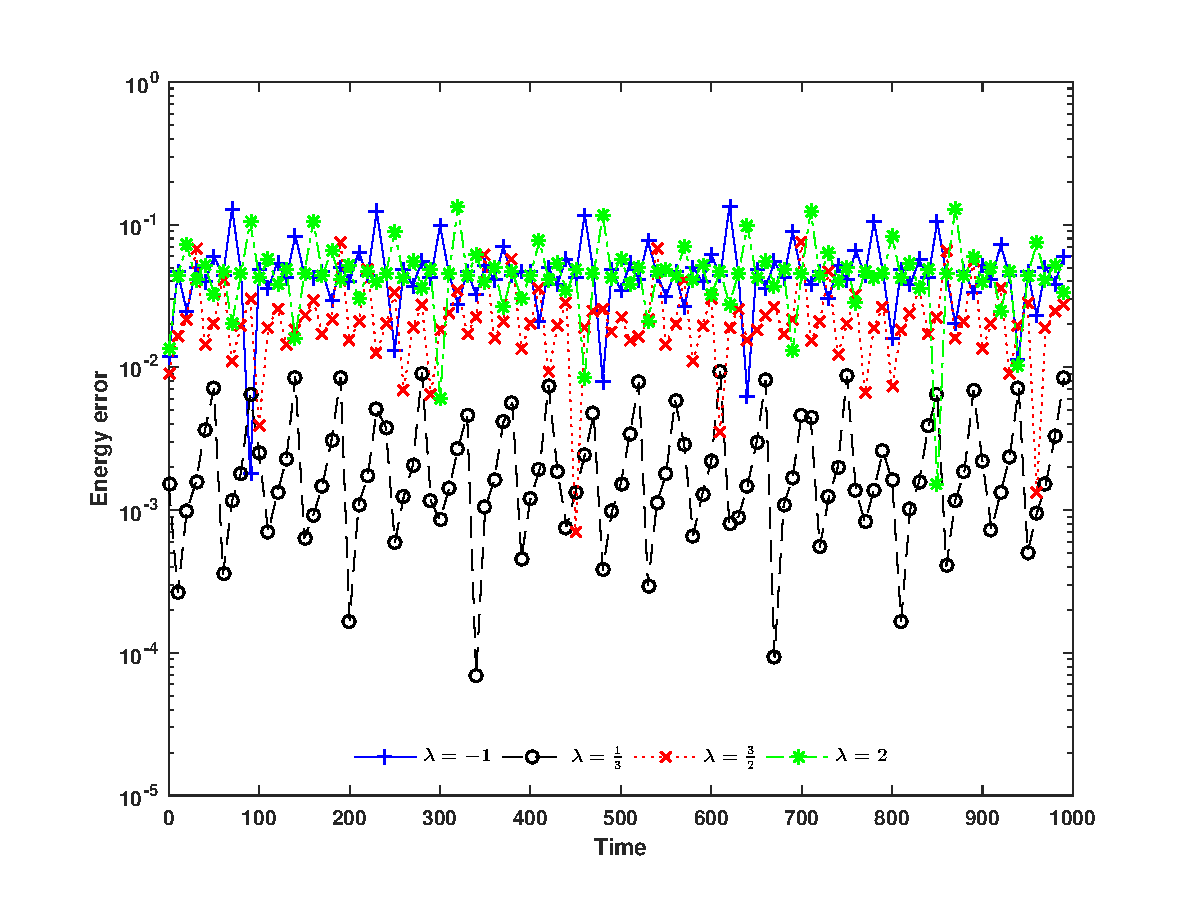
\includegraphics[width=42mm]{perKepler_sym_HE}\\
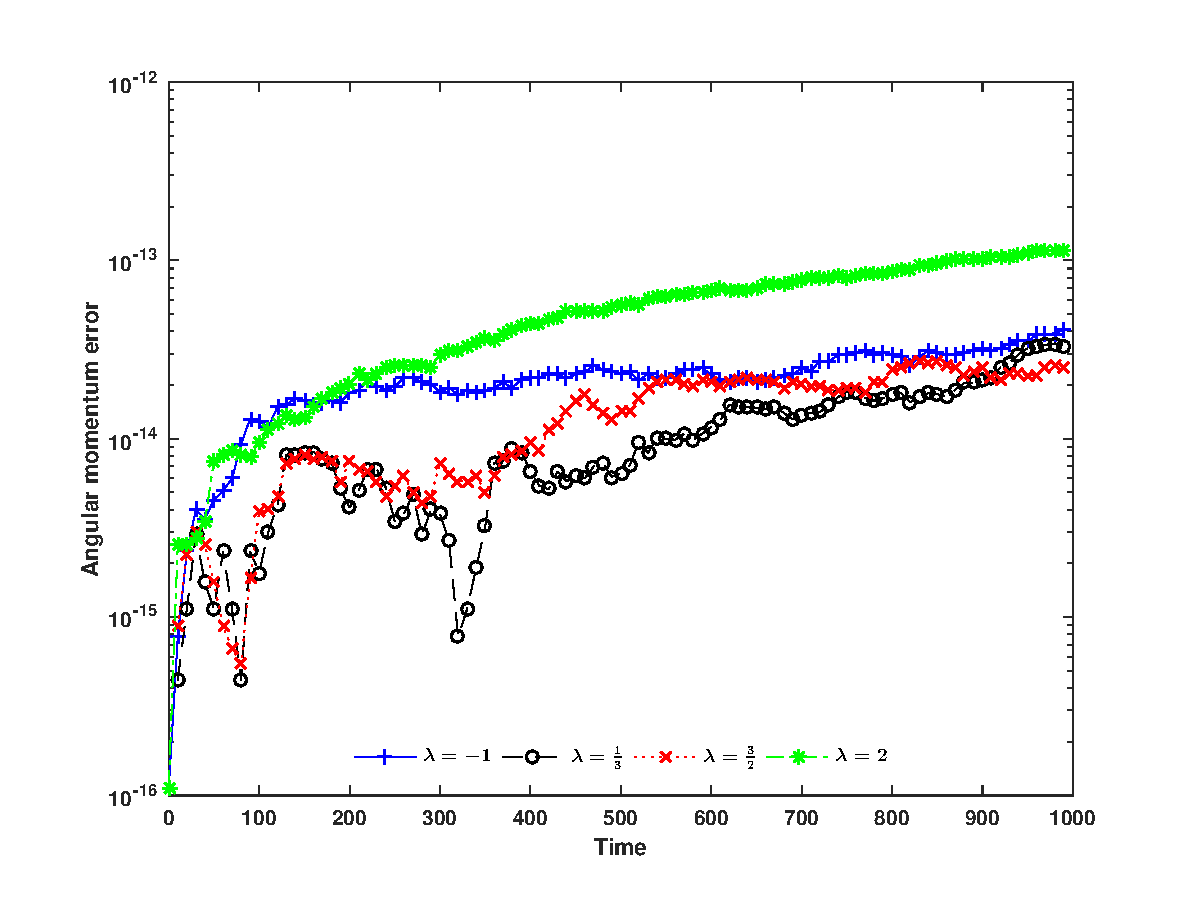
\includegraphics[width=42mm]{perKepler_sym_LE}
\end{minipage}}
\subfigure[Scheme III (right)]{
\begin{minipage}[t]{0.33\textwidth}
\centering
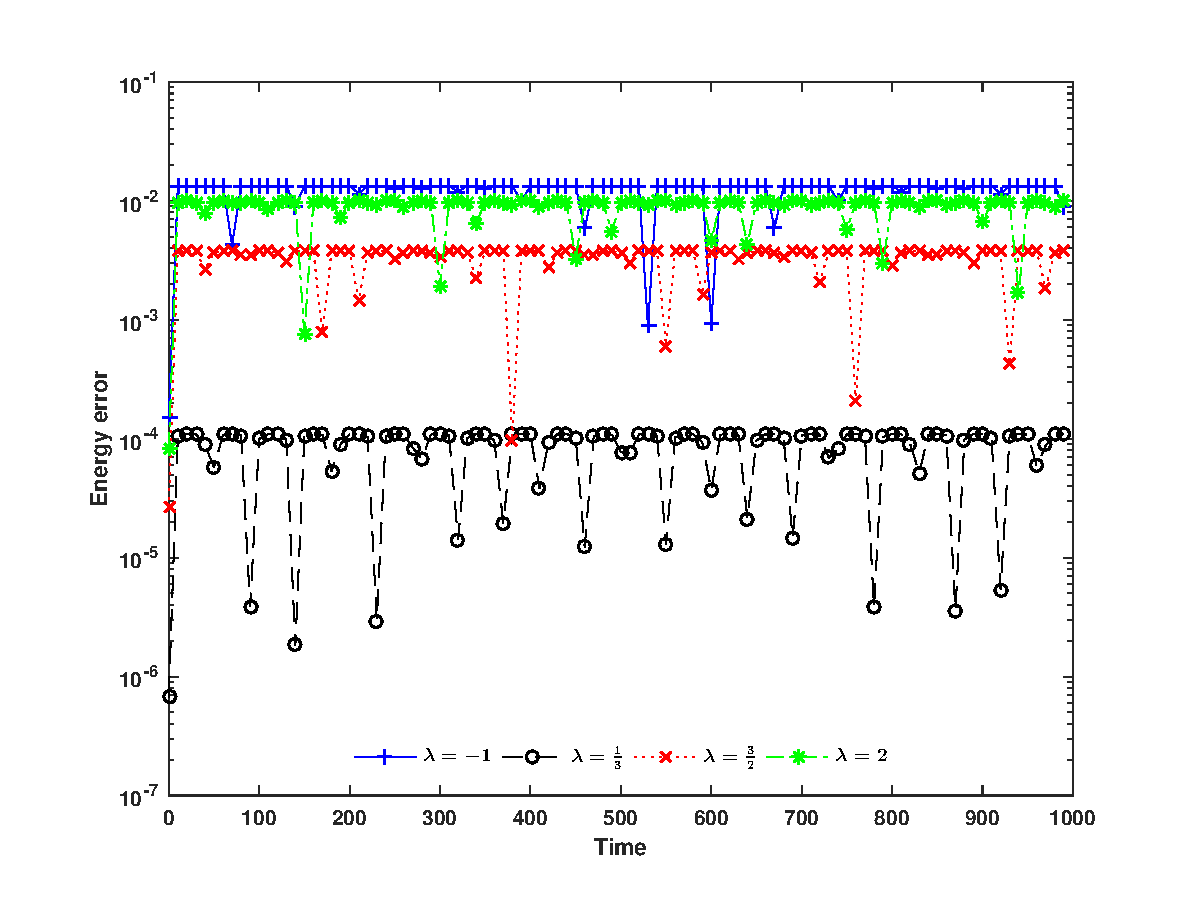
\includegraphics[width=42mm]{perKepler2_sym_HE}\\
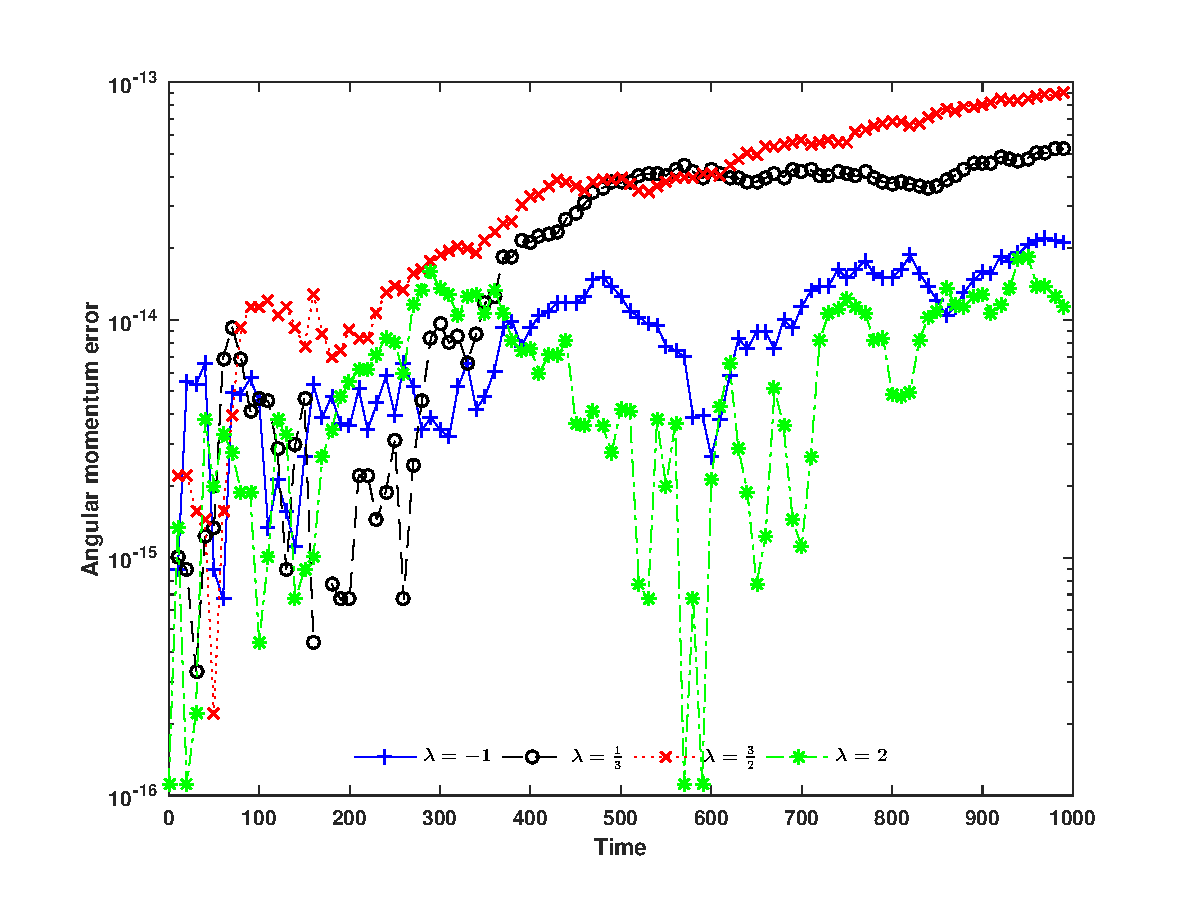
\includegraphics[width=42mm]{perKepler2_sym_LE}
\end{minipage}}
\end{figure}
\end{frame}

\begin{frame}{Numerical experiments: the sine-Gordon equation}
We test the the sine-Gordon equation in the form
\begin{equation*}
u_{tt}-\triangle u+\mbox{sin}\left(u\right)=0,\quad (x,y)\in\Omega\in\mathcal{R}^2,\ t\in (0,T]
\end{equation*} 
with periodic boundary conditions. The two different initial conditions are carried out by selecting
\begin{itemize}
\item Circular ring soliton: $\Omega=[-7,7)\times[-7,7)$,
\begin{align*}
\aligned
&u(x,y,0)=4\ \mbox{tan}^{-1}\bigg(\mbox{exp}\left(3-\sqrt{x^2+y^2}\right)\bigg),\\
&u_t(x,y,0)=0;
\endaligned
\end{align*}
\item Collision of four circular solitons: $\Omega=[-30,10)\times[-30,10)$,
\begin{align*}
\aligned
&u(x,y,0)=4\ \mbox{tan}^{-1}\mbox{exp}\bigg[\left(4-\sqrt{(x+3)^2+(y+3)^2}\right)/0.436\bigg],\\
&u_t(x,y,0)=4.13\ \mbox{sech}\bigg[\left(4-\sqrt{(x+3)^2+(y+3)^2}\right)/0.436\bigg].
\endaligned
\end{align*}
\end{itemize} 
\end{frame}

\begin{frame}{Circular ring soliton of Scheme I}
\begin{figure}
\centering
\subfigure[$T=0$]{
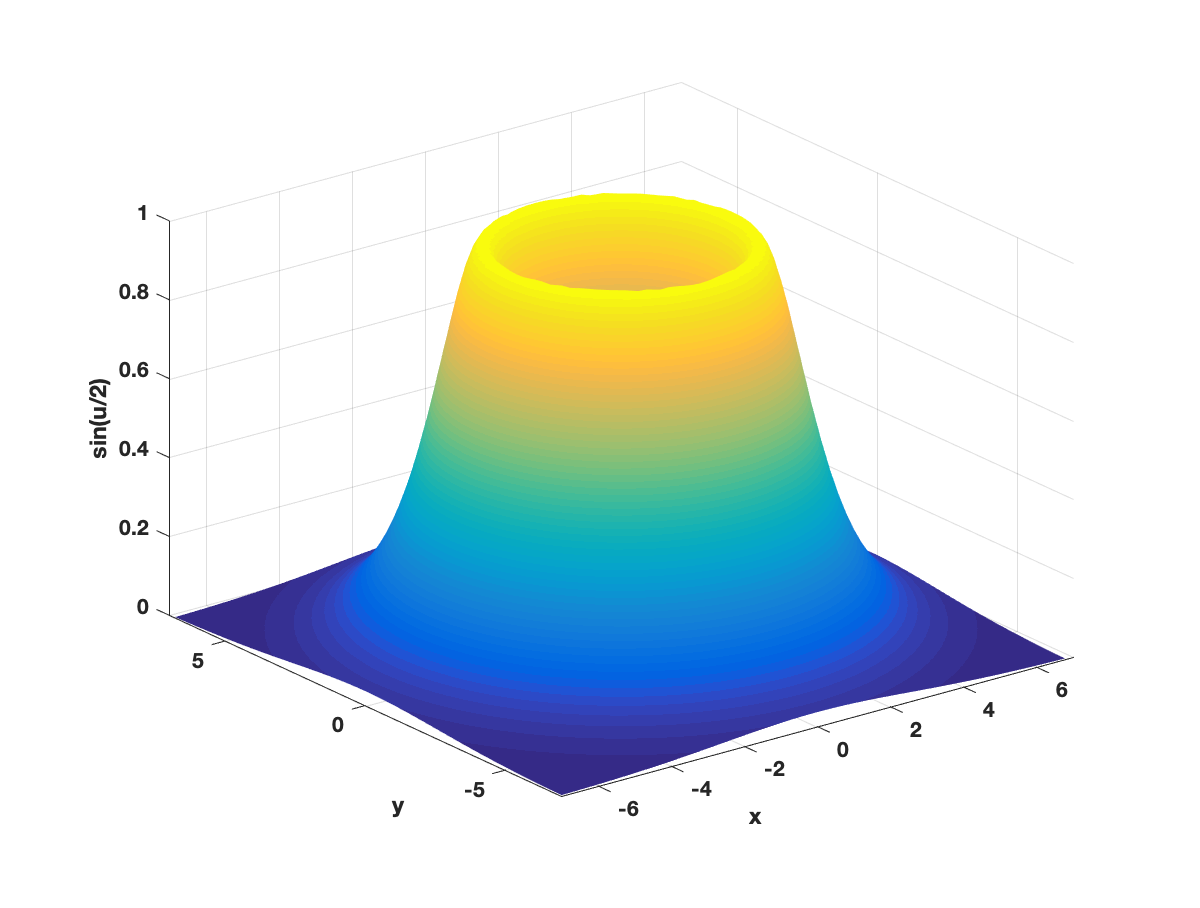
\includegraphics[width=0.33\textwidth]{CRS_solu_0_sym}}\hspace{-4mm}
\subfigure[$T=2.8$]{
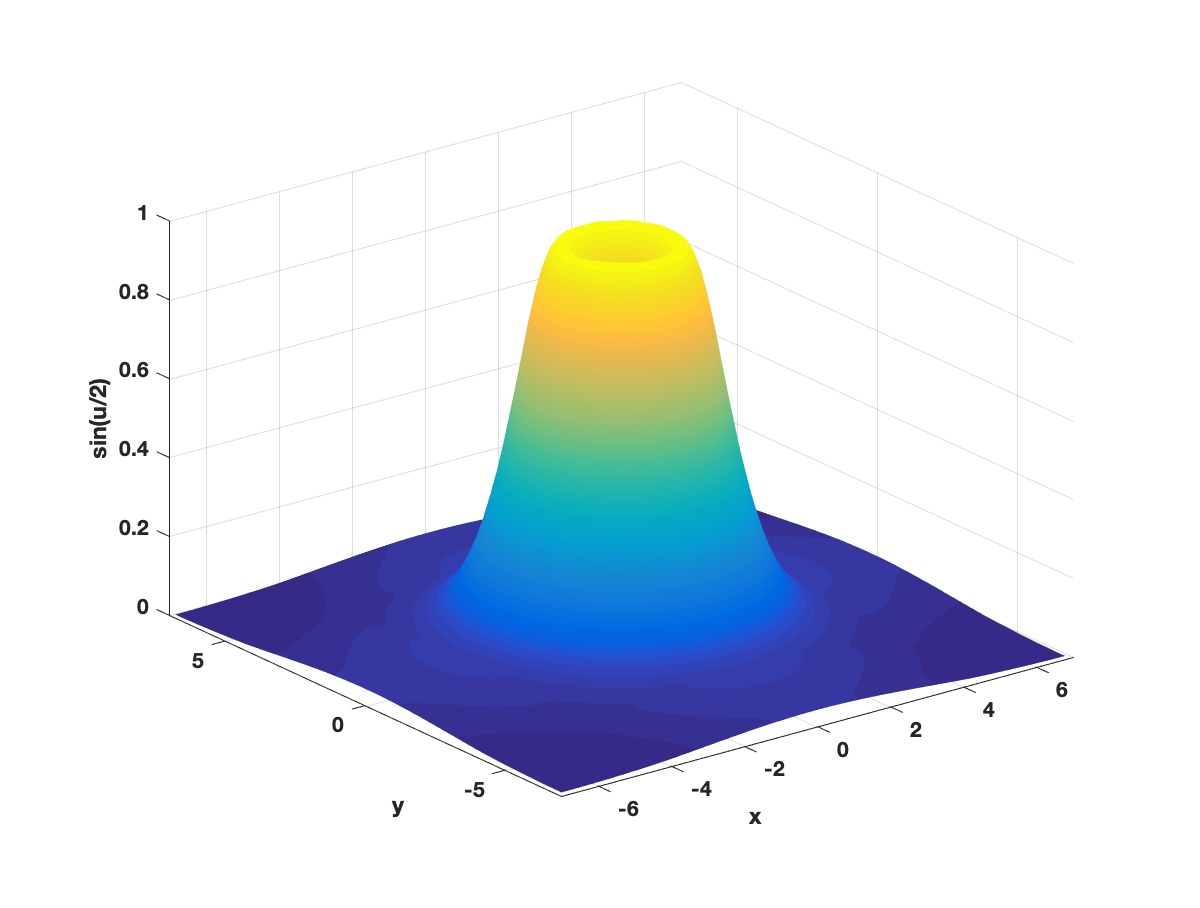
\includegraphics[width=0.33\textwidth]{CRS_solu_1_sym}}\hspace{-4mm}
\subfigure[$T=5.6$]{
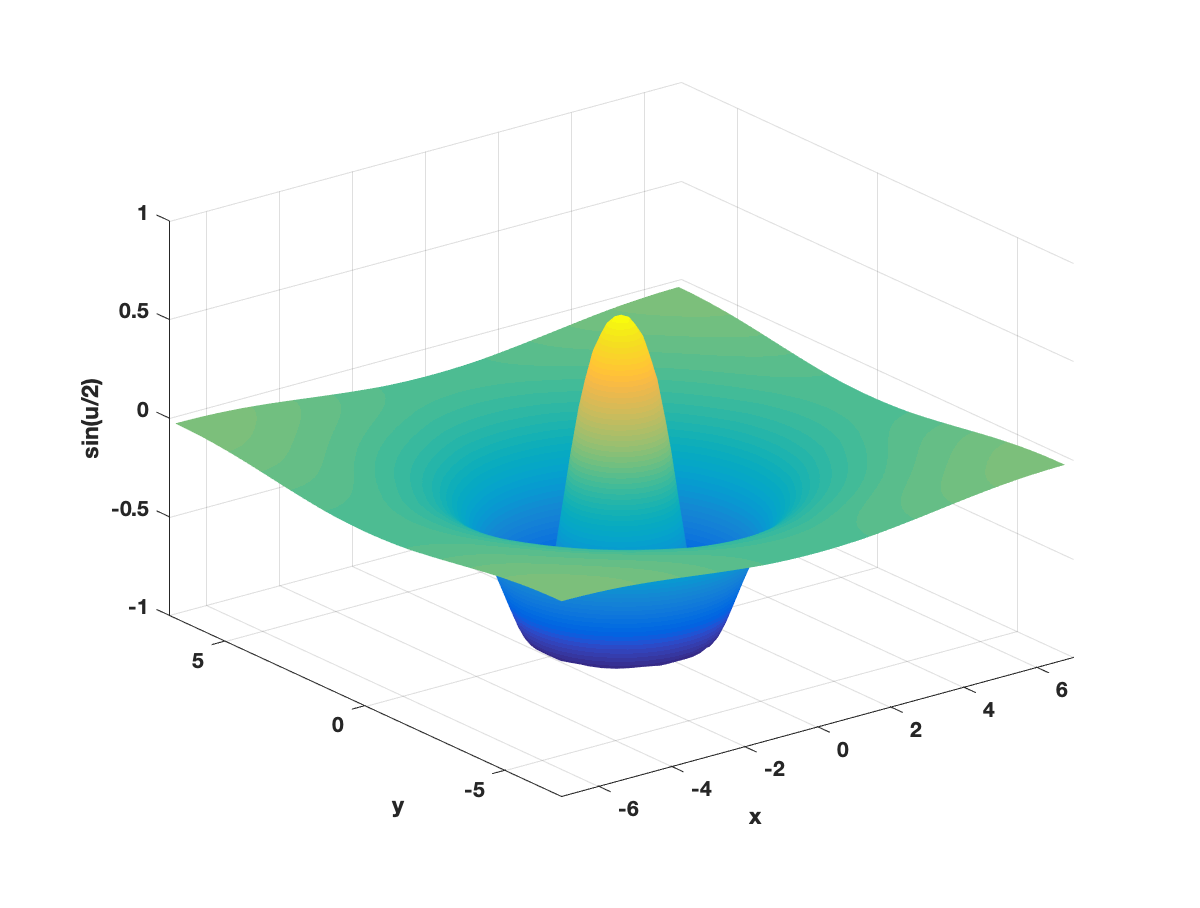
\includegraphics[width=0.33\textwidth]{CRS_solu_2_sym}}\vspace{-1mm}
\subfigure[$T=8.4$]{
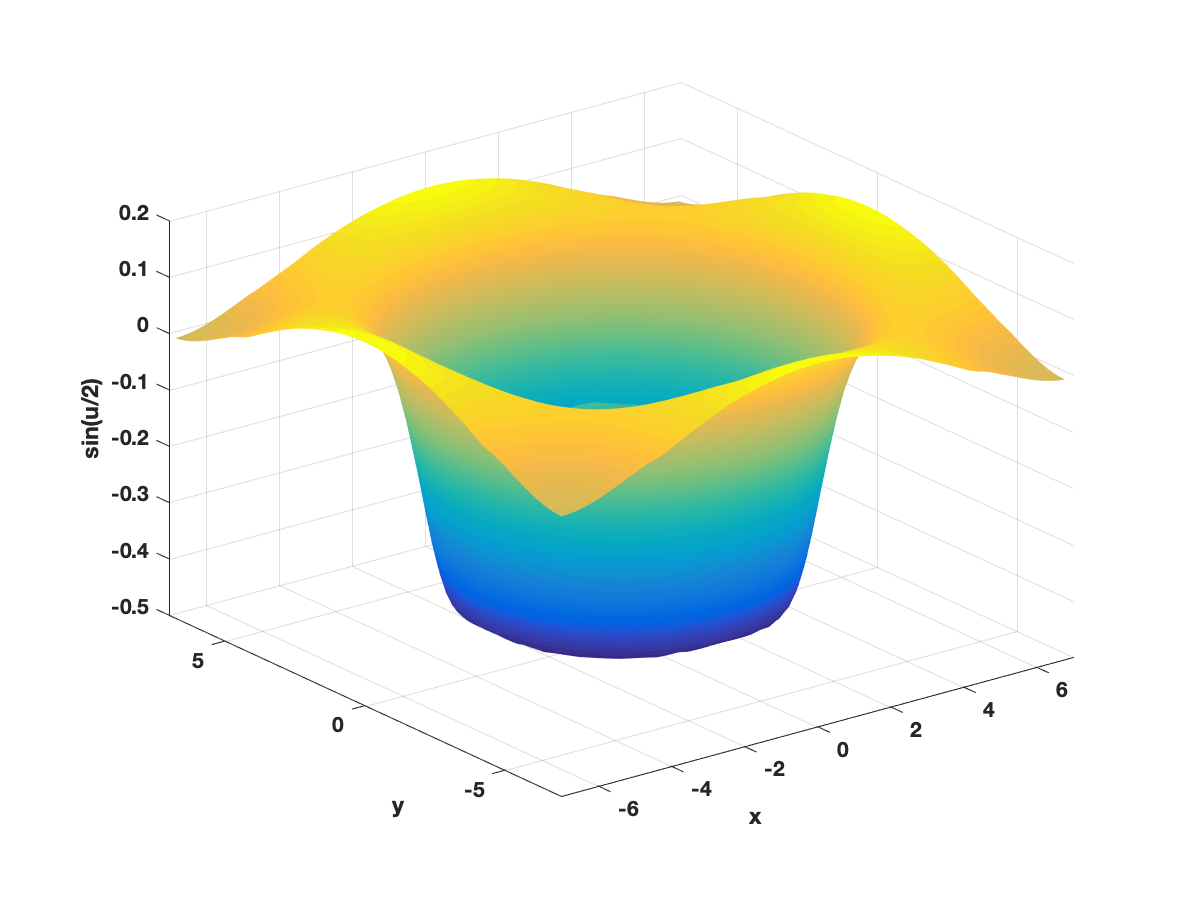
\includegraphics[width=0.33\textwidth]{CRS_solu_3_sym}}\hspace{-4mm}
\subfigure[$T=11.2$]{
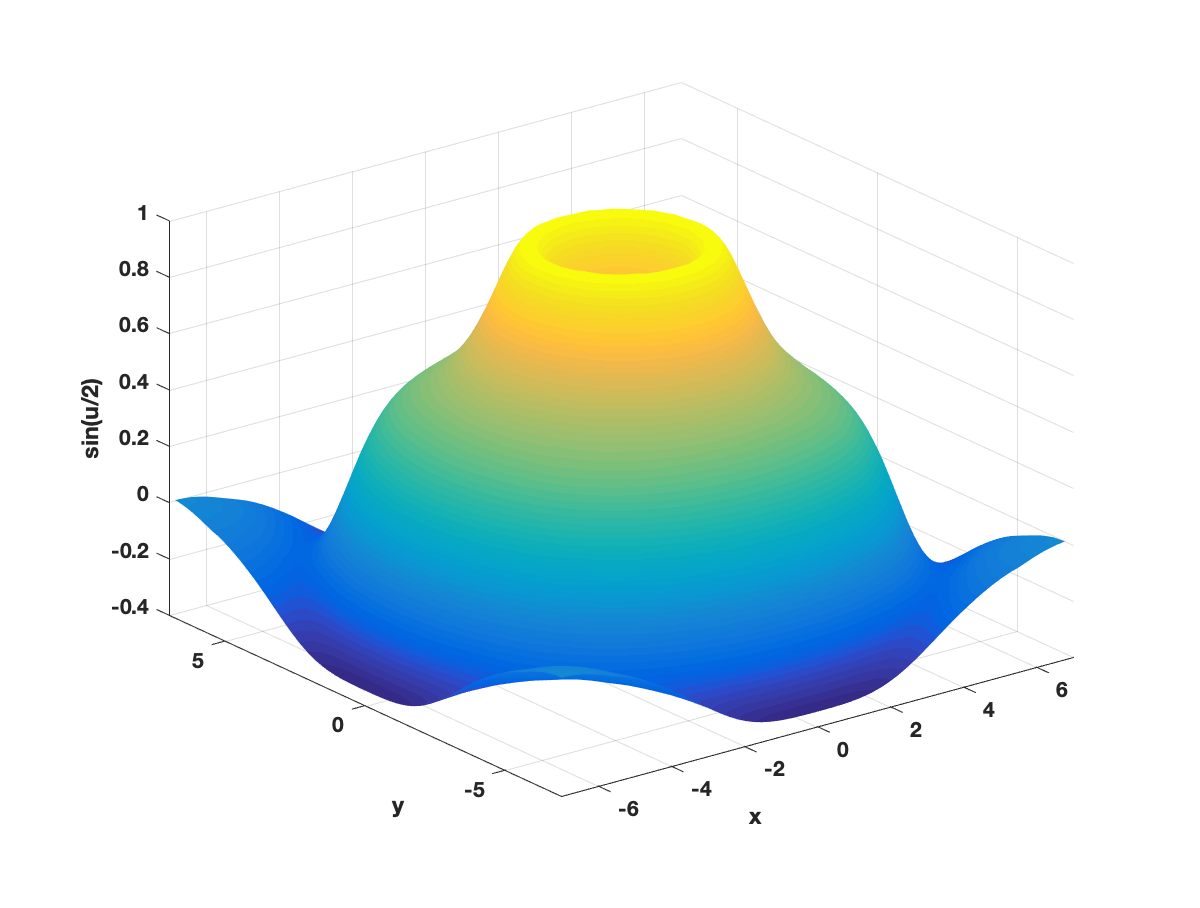
\includegraphics[width=0.33\textwidth]{CRS_solu_4_sym}}\hspace{-4mm}
\subfigure[$T=12.6$]{
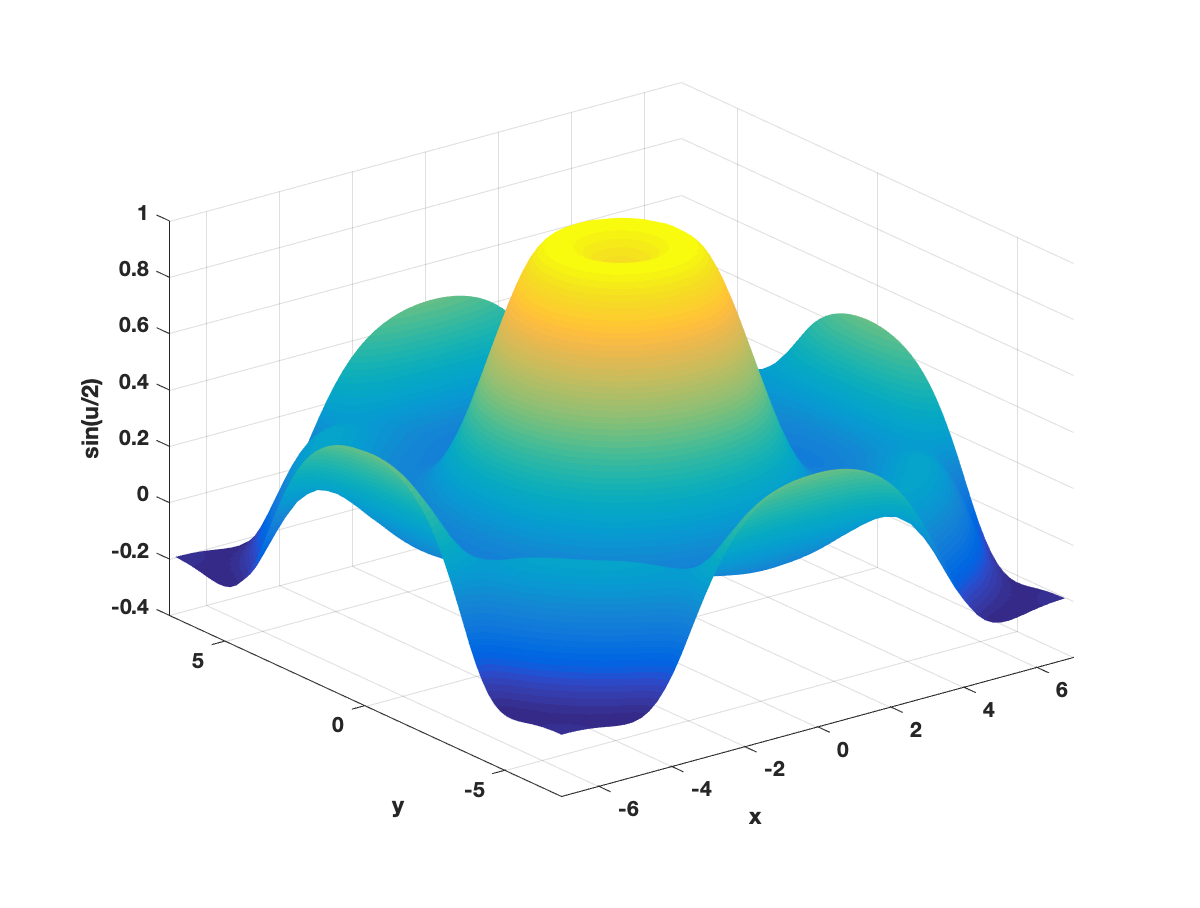
\includegraphics[width=0.33\textwidth]{CRS_solu_5_sym}}
\end{figure}	
\end{frame}

\begin{frame}{Collision of four circular solitons of Scheme I}
\begin{figure}
\centering
\subfigure[$T=0$]{
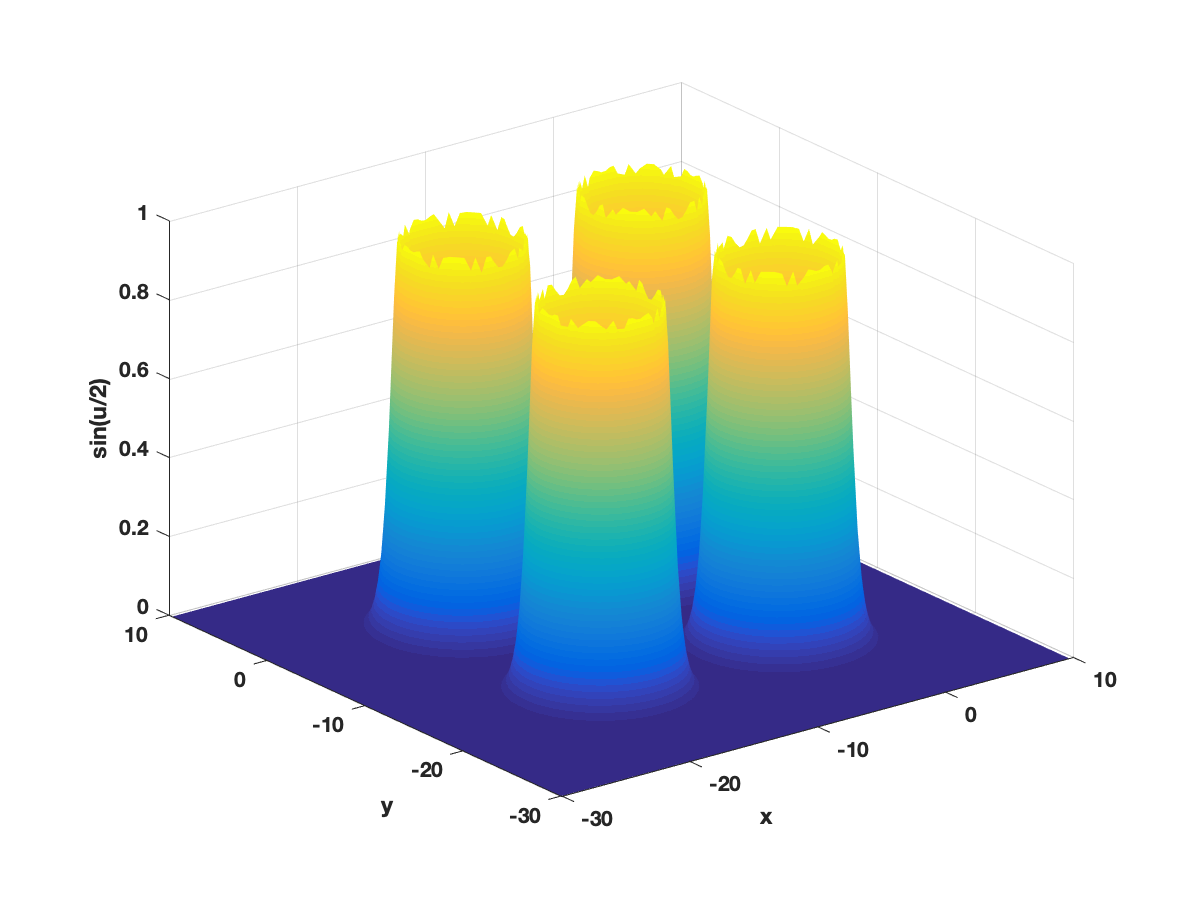
\includegraphics[width=0.33\textwidth]{CCS_solu_0_sym}}\hspace{-4mm}
\subfigure[$T=2.5$]{
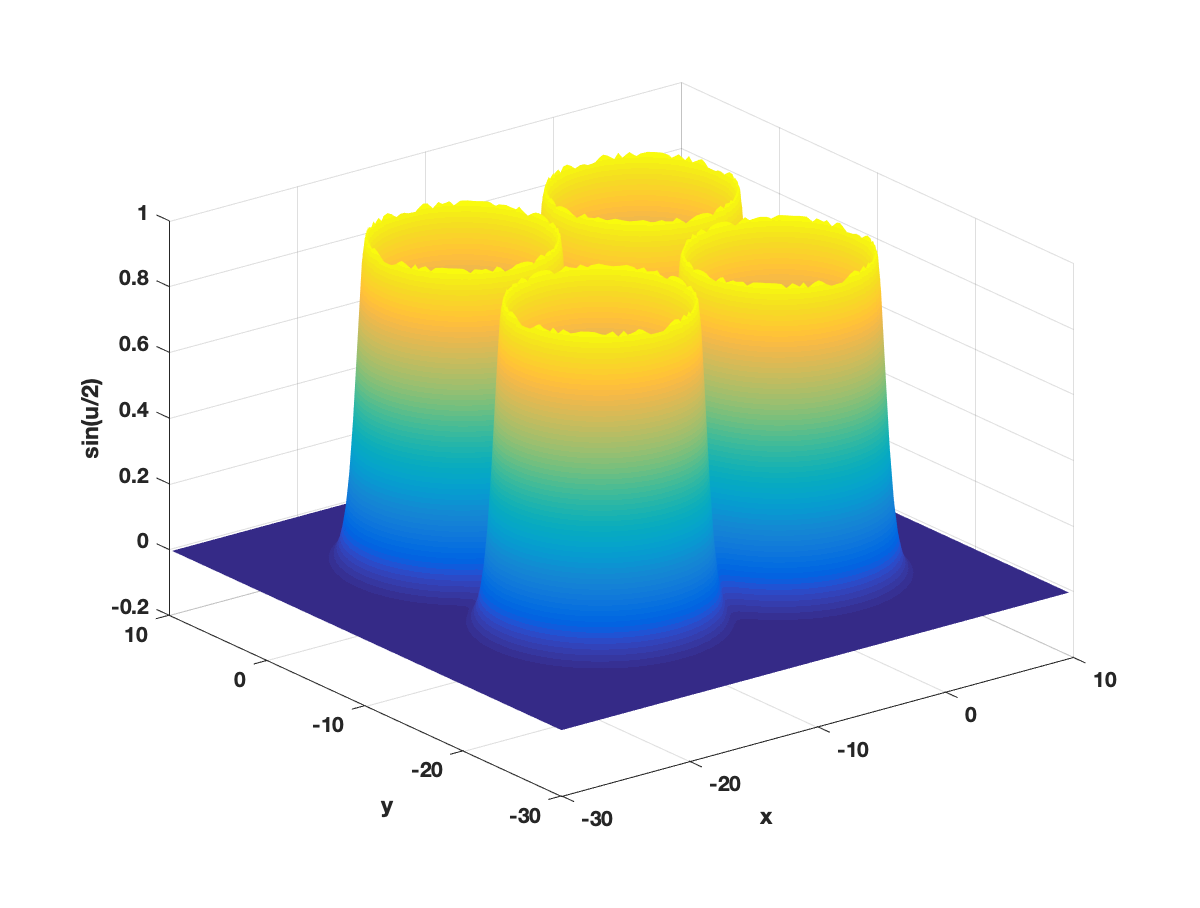
\includegraphics[width=0.33\textwidth]{CCS_solu_1_sym}}\hspace{-4mm}
\subfigure[$T=5$]{
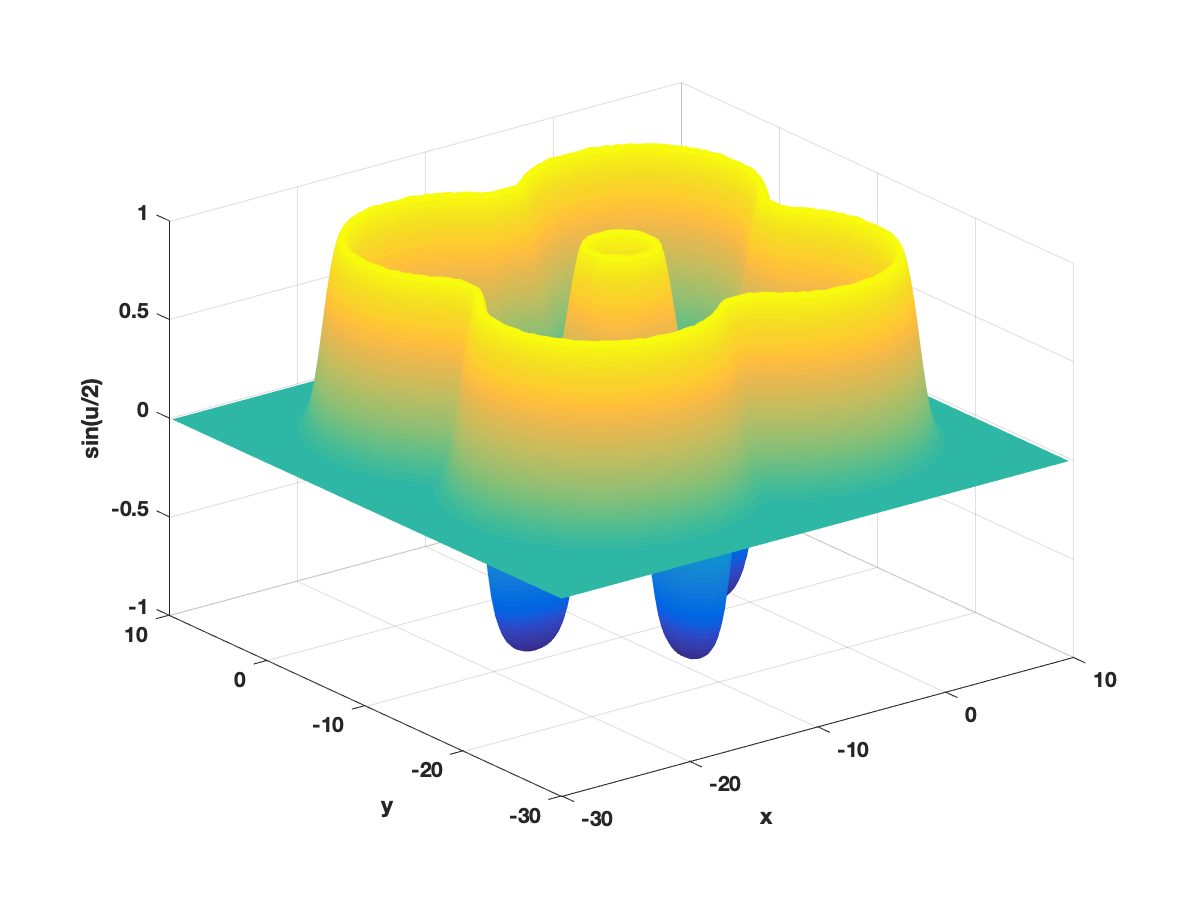
\includegraphics[width=0.33\textwidth]{CCS_solu_2_sym}}\vspace{-1mm}
\subfigure[$T=7.5$]{
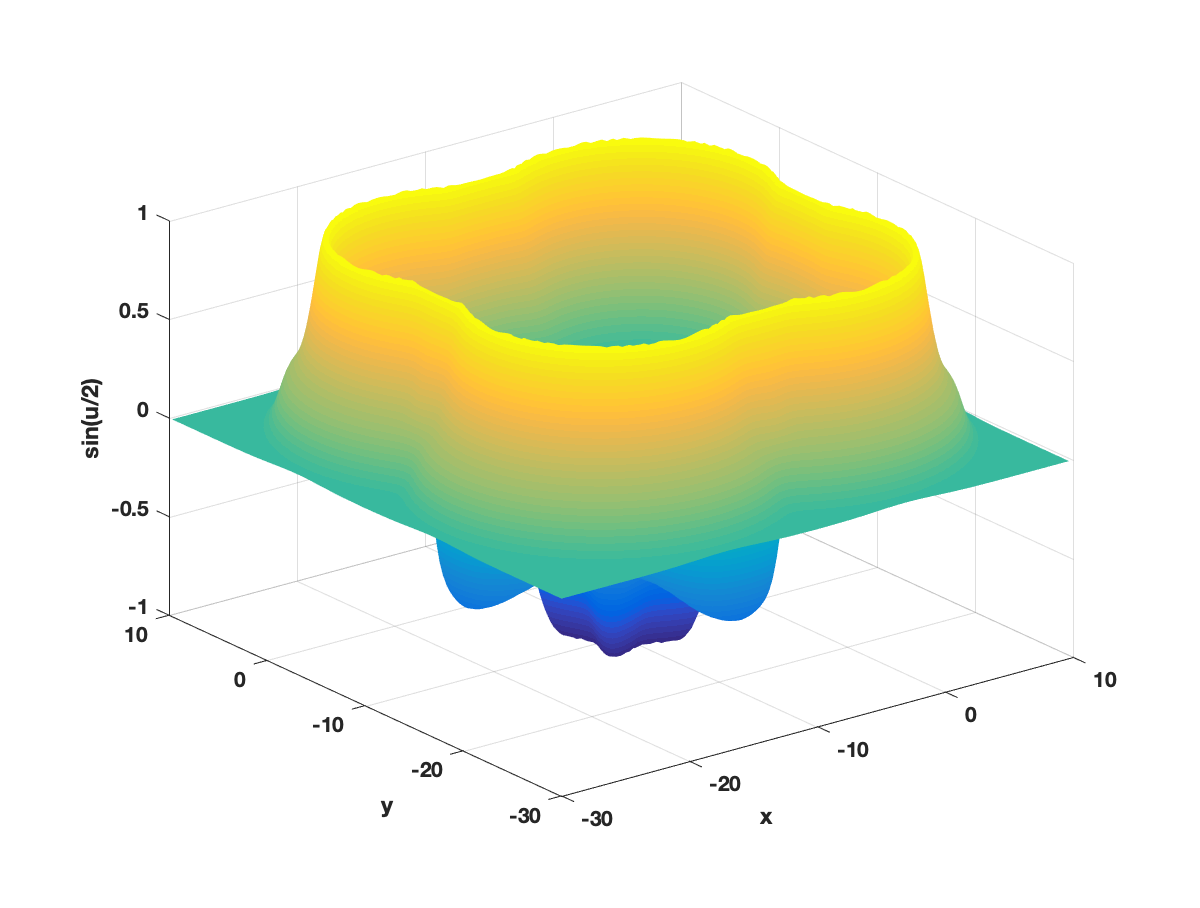
\includegraphics[width=0.33\textwidth]{CCS_solu_3_sym}}\hspace{-4mm}
\subfigure[$T=10$]{
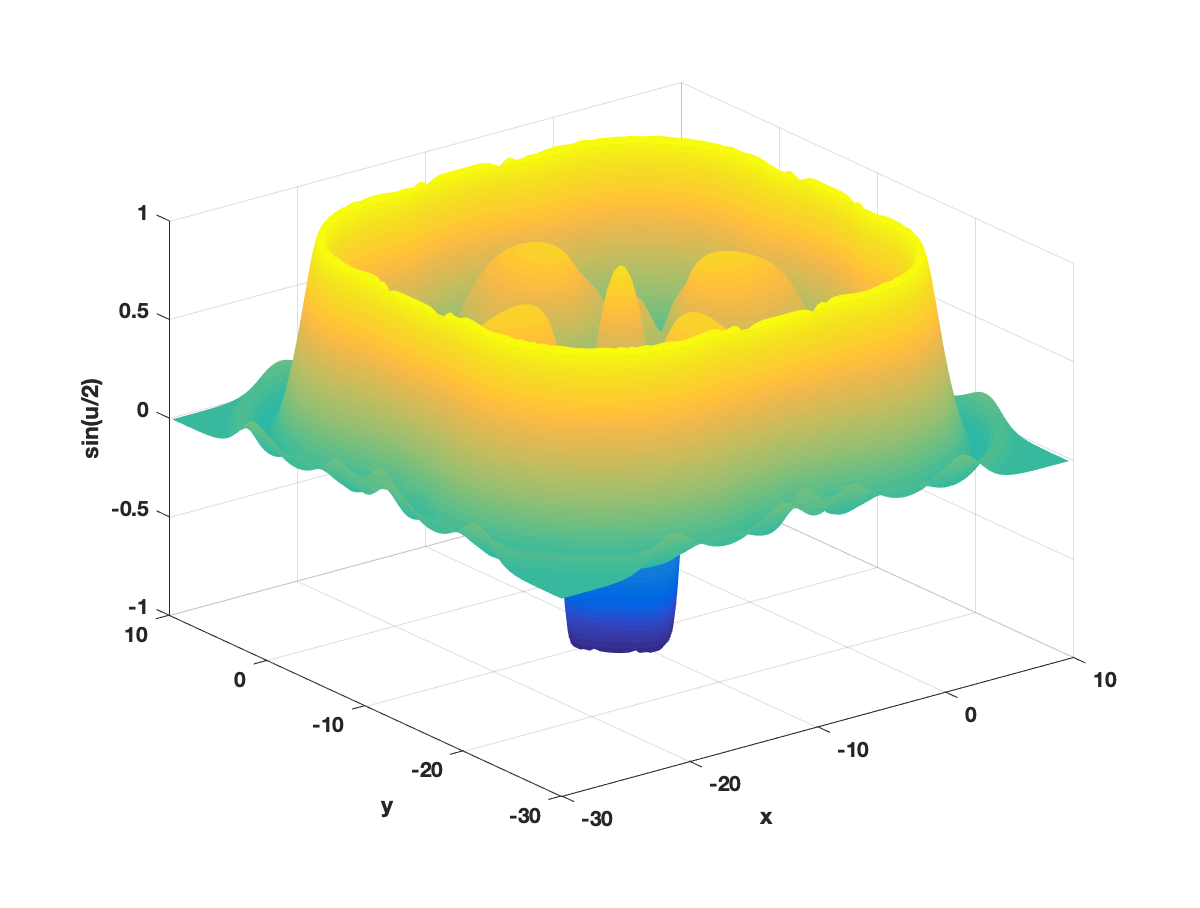
\includegraphics[width=0.33\textwidth]{CCS_solu_4_sym}}
\end{figure}	
\end{frame}		

\begin{frame}{Energy errors of Scheme I}	
\begin{figure}
\centering
\subfigure[Circular ring soliton]{
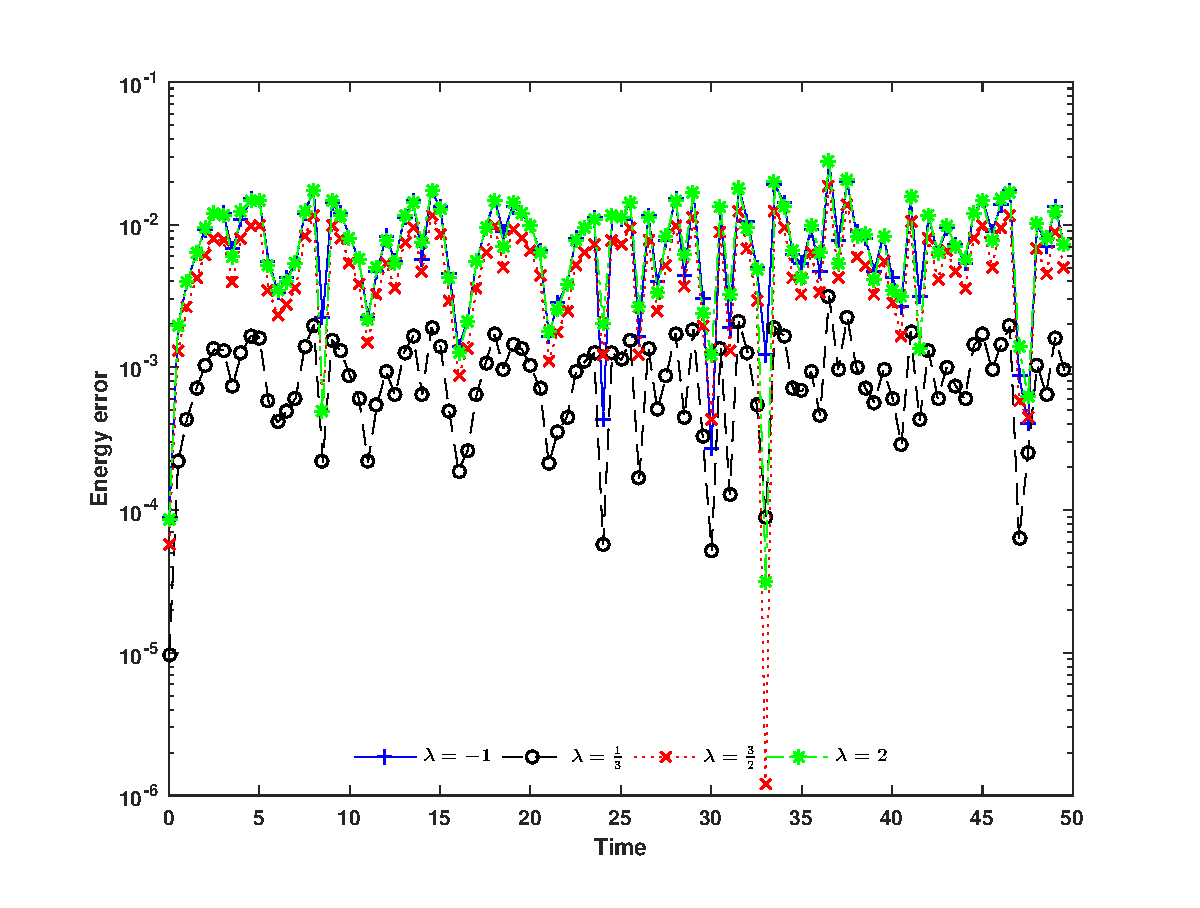
\includegraphics[width=0.45\textwidth]{CRS_sym_HE}}\hspace{-2mm}
\subfigure[Collision of four circular solitons]{
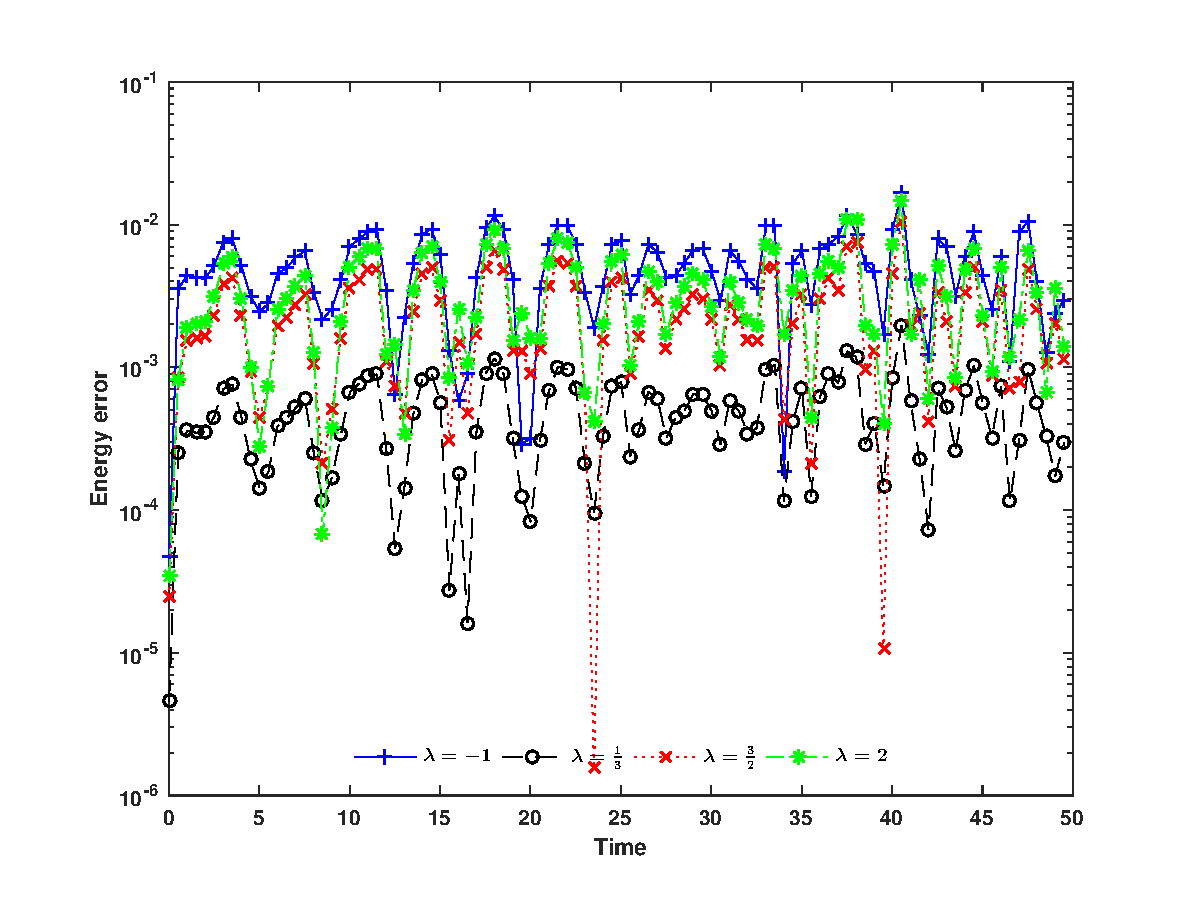
\includegraphics[width=0.45\textwidth]{CCS_sym_HE}}
\end{figure}
\end{frame}	


\section{Arbitrary high-order energy and quadratic invariants preserving methods}
\begin{frame}{Energy and quadratic invariants preserving methods (EQUIP)\footnote{Y.H. Bo, W.J. Cai, and Y.S. Wang. arXiv:1912.00727, 2020.}}
Two families of one-step methods depending on a free parameter are constructed such that each method is symplectic for any fixed parameter, and that a special value of the parameter can be chosen with the energy conservation at the same time.\\
\vspace{2mm}
\textcolor[rgb]{0,0,1}{$\blacktriangleright$} \textcolor{blue}{Scheme EI:}
\begin{align}\label{eq-22}
\aligned
&p_{n+1}=p_n-\tau\partial_qH\big(\lambda p_{n+1}+(1-\lambda)p_n,\lambda q_n+(1-\lambda)q_{n+1}\big),\\
&q_{n+1}=q_n+\tau\partial_pH\big(\lambda p_{n+1}+(1-\lambda)p_n,\lambda q_n+(1-\lambda)q_{n+1}\big),\\
&H(p_{n+1},q_{n+1})=H(p_n,q_n).
\endaligned
\end{align}

\textcolor[rgb]{0,0,1}{$\blacktriangleright$} \textcolor{blue}{Scheme EII:}
\begin{align}\label{eq-23}
\aligned
&(p_{n+1},q_{n+1})=\Psi_\tau(p_n,q_n),\\
&H(p_{n+1},q_{n+1})=H(p_n,q_n),
\endaligned
\end{align}
where $\Psi_\tau$ is Scheme III as the composition of Scheme I and its adjoint method.
\end{frame}

\begin{frame}
If a real value $\lambda_*$ can be found such that $H(p_{n+1},q_{n+1}) = H(p_n,q_n)$ is satisfied, we get a one-step scheme
\begin{equation}\label{eq-24}
\Phi_\tau^{\lambda_*}: (p_n,q_n) \mapsto (p_{n+1},q_{n+1}).
\end{equation} 
For a fixed $\lambda_*$, the scheme \eqref{eq-24} is symplectic so that all quadratic invariants are preserved. If the existence of the parameter $\lambda_*$ is verified, there exists a real sequence \{$\lambda_i$\} as the following diagram
\begin{equation}\label{eq-25}
(p_n,q_n) \stackrel{\Phi_\tau^{\lambda_1}}{\longmapsto} (p_{n+1},q_{n+1}) \stackrel{\Phi_\tau^{\lambda_2}}{\longmapsto} (p_{n+2},q_{n+2}) \stackrel{\Phi_\tau^{\lambda_3}}{\longmapsto} (p_{n+3},q_{n+3}) \longmapsto \cdots
\end{equation}
such that the numerical solution $(p_{n+i},q_{n+i})$ defined by $\Phi_h^{\lambda_i}$ satisfies $H(p_{n+i},q_{n+i})=H(p_n,q_n)$, $i=1,2,\cdots$. Symplectic schemes with different fixed parameters are used at each step to obtain energy conservation. 

\begin{remark}
Schemes EI and EII are energy and quadratic invariants preserving.
\end{remark}
\end{frame}

\begin{frame}{Solvability}
Following the classical formulation of the implicit function theorem, we define the vector equation
\begin{equation}\label{eq-26}
G(p_{n+1},q_{n+1},\lambda,p_n,q_n,\tau)=
\left(
\begin{array}{c}
p_{n+1}-p_n+\tau H_q(\bar{u},\bar{v})\\
q_{n+1}-q_n-\tau H_p(\bar{u},\bar{v})\\
H(p_{n+1},q_{n+1})-H(p_n,q_n)
\end{array}\right)=0
\end{equation}
which is equivalent to Scheme EI. The function $G$ vanishes at $(p_n,q_n,\lambda_0,p_n,q_n,0)$ with any real $\lambda_0$. The Jacobian of $G$ is obtained as
\begin{equation}\label{eq-27}
\frac{\partial G}{\partial(p_{n+1},q_{n+1},\lambda)}\bigg|_{(p_n,q_n,\lambda_0,p_n,q_n,0)} =
\left ( \begin{array}{ccc}
\mathcal{I} & 0 & 0\\
0 & \mathcal{I} & 0\\
H_p(p_n,q_n) & H_q(p_n,q_n) & 0
\end{array}\right).
\end{equation}
This lead to a nonlinear system with a \textcolor{blue}{singular Jacobian} so the usual Newton-type iteration methods are invalid.
\end{frame}

\begin{frame}
The nonlinear function
\begin{equation}\label{eq-28}
E(\lambda,\tau)=H\big(p_{n+1}(\lambda,\tau),q_{n+1}(\lambda,\tau)\big)-H(p_n,q_n)
\end{equation}
is introduced as an error of the numerical Hamiltonian, where $p_{n+1}(\lambda,\tau)$ and $q_{n+1}(\lambda,\tau )$ are defined by Scheme I.\\
\vspace{4mm}
It is apparent that the solvability of Scheme EI is equivalent to the existence of a solution in the form $\lambda_*=\lambda_*(\tau)$ of $E(\lambda,\tau)=0$, in particular $E(1/2,0)=0$ as the initial condition.\\
\vspace{4mm}
\begin{theorem}
Assuming that the Hamiltonian is sufficiently smooth, then there exists a function $\lambda_*$=$\lambda_*(\tau)$ defined in a neighborhood $(-\tau_0,\tau_0)$ with $\tau_0$ small enough, such that\\
\vspace{1mm}
\quad (1) $E\big(\lambda_*(\tau),\tau\big)=0$ for all $\tau \in (-\tau_0,\tau_0)$;\\
\vspace{1mm}
\quad (2) $\lambda_*(\tau)=1/2+\varepsilon(\tau)\tau$ with $\varepsilon(\tau)=\text{constant}+\mathcal{O}(\tau)$.
\end{theorem} 
\end{frame}

\begin{frame}{Concluding remarks}
\quad\textcolor[rgb]{0,0,1}{$\bullet$} The existence of \textcolor{blue}{$\lambda_*(\tau)=1/2+\varepsilon(\tau)\tau$ around $1/2$} is confirmed to make EQUIP methods solvable, which reveals the superior behavior of the midpoint method in most actual calculations.\\  
\vspace{4mm}
\quad\textcolor[rgb]{0,0,1}{$\bullet$} By tuning the free parameter in symplectic schemes, we achieve the energy preservation. Thus, we establish the relation between symplectic schemes and energy-preserving methods.\\
\vspace{4mm}
\quad\textcolor[rgb]{0,0,1}{$\bullet$} A novel methodology is proposed to construct arbitrary high-order energy preserving methods.\\
\vspace{4mm}
\quad\textcolor[rgb]{0,0,1}{$\bullet$} Different from the time-adaptive strategy, symplectic and energy conservation are realized at the same time from a new perspective in a weaker sense.
\end{frame}

\begin{frame}{Numerical experiments: the H\'{e}non-Heiles model}
\begin{figure}
\centering
\subfigure[AVF (left)]{
\begin{minipage}[t]{0.33\textwidth}
\centering
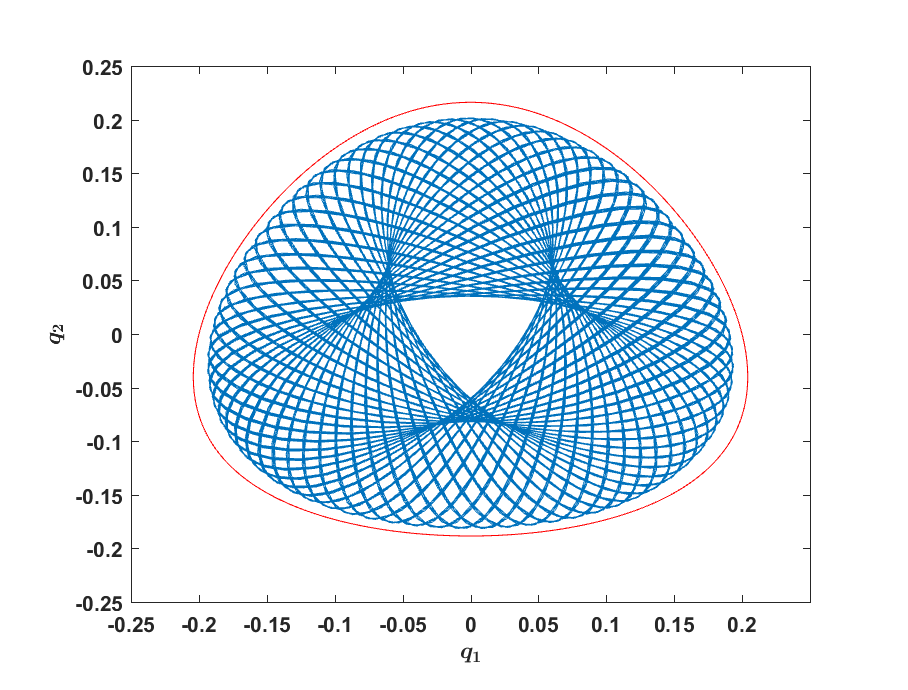
\includegraphics[width=42mm]{AVF_bHH_R}\\
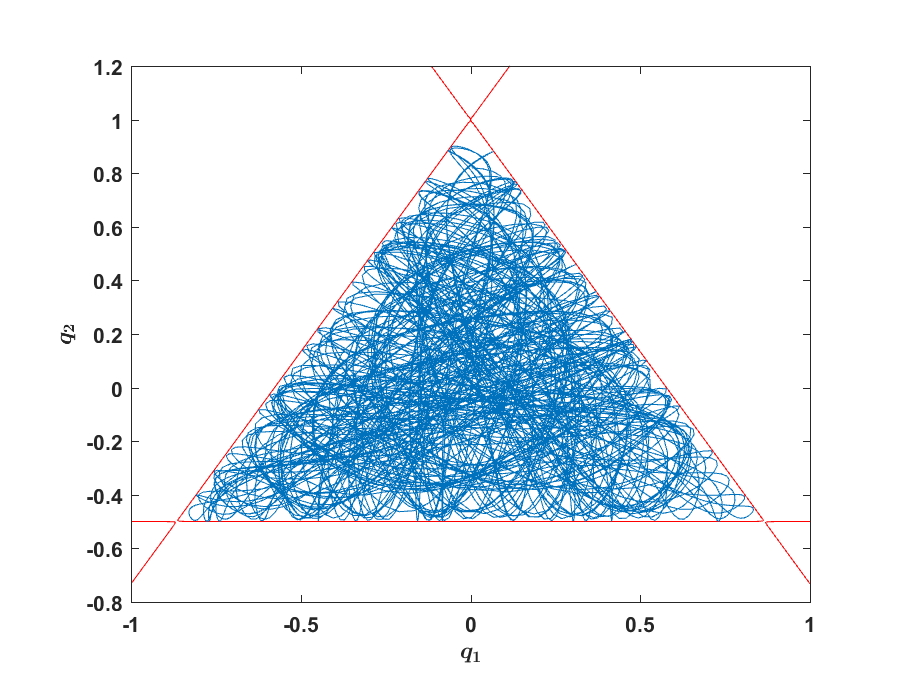
\includegraphics[width=42mm]{AVF_cHH_R}
\end{minipage}}\hspace{-3.2mm}
\subfigure[Scheme EI (middle)]{
\begin{minipage}[t]{0.33\textwidth}
\centering
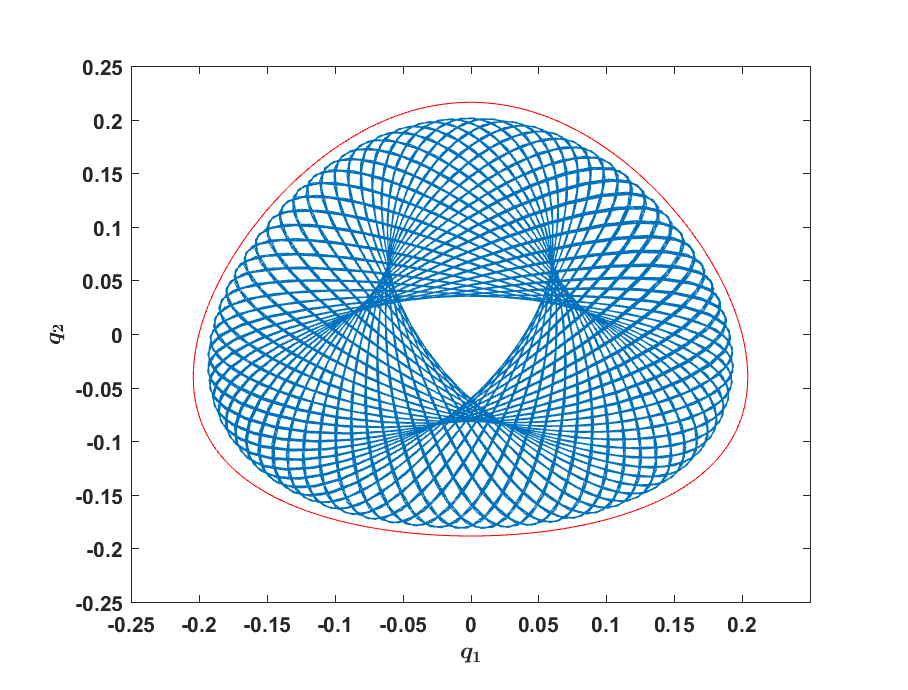
\includegraphics[width=42mm]{bHH_R}\\
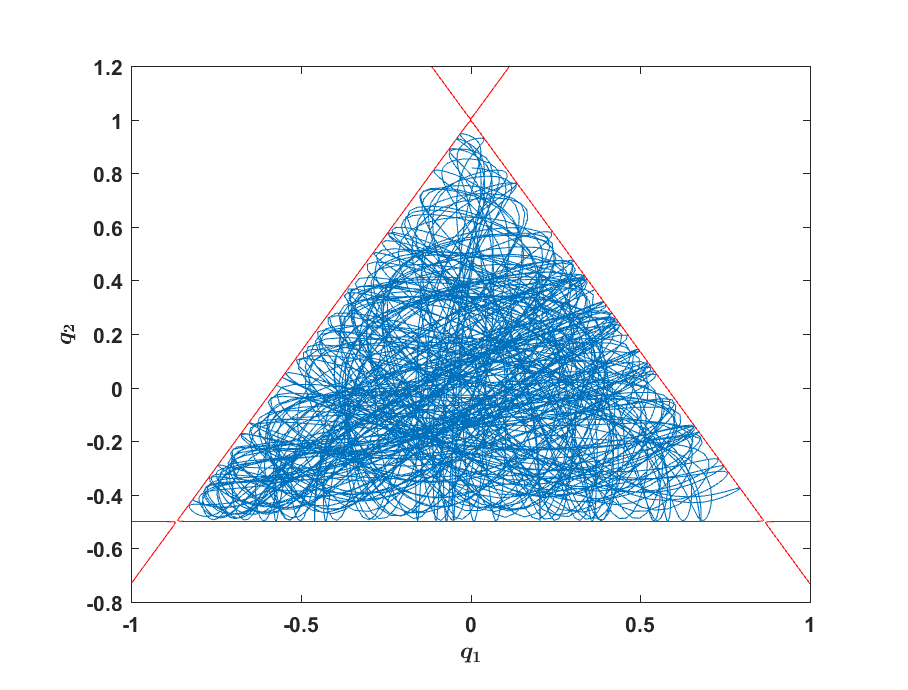
\includegraphics[width=42mm]{cHH_R}
\end{minipage}}\hspace{-3.2mm}
\subfigure[Scheme EII (right)]{
\begin{minipage}[t]{0.33\textwidth}
\centering
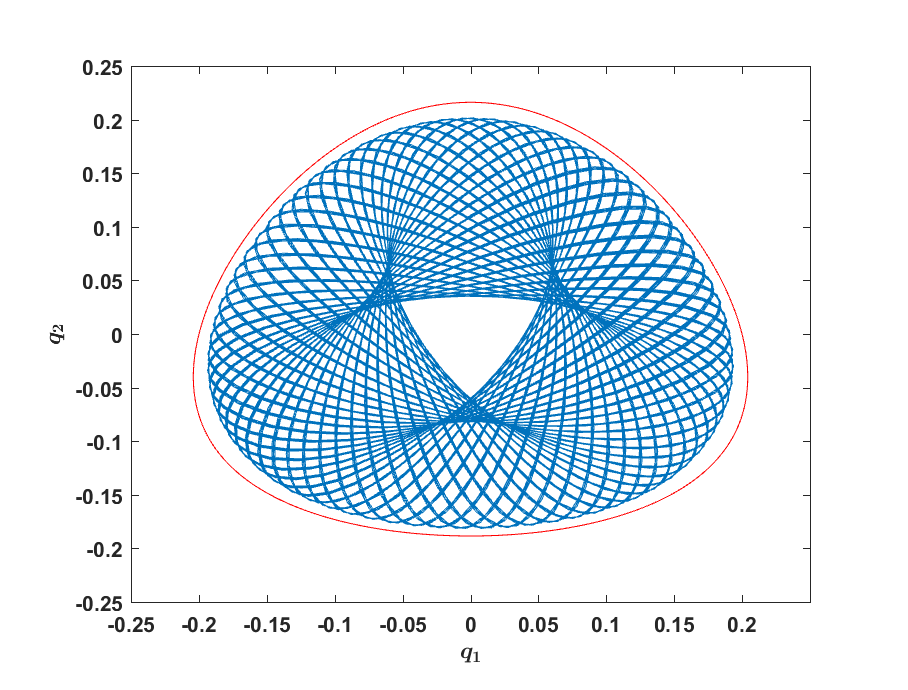
\includegraphics[width=42mm]{bHH2_R}\\
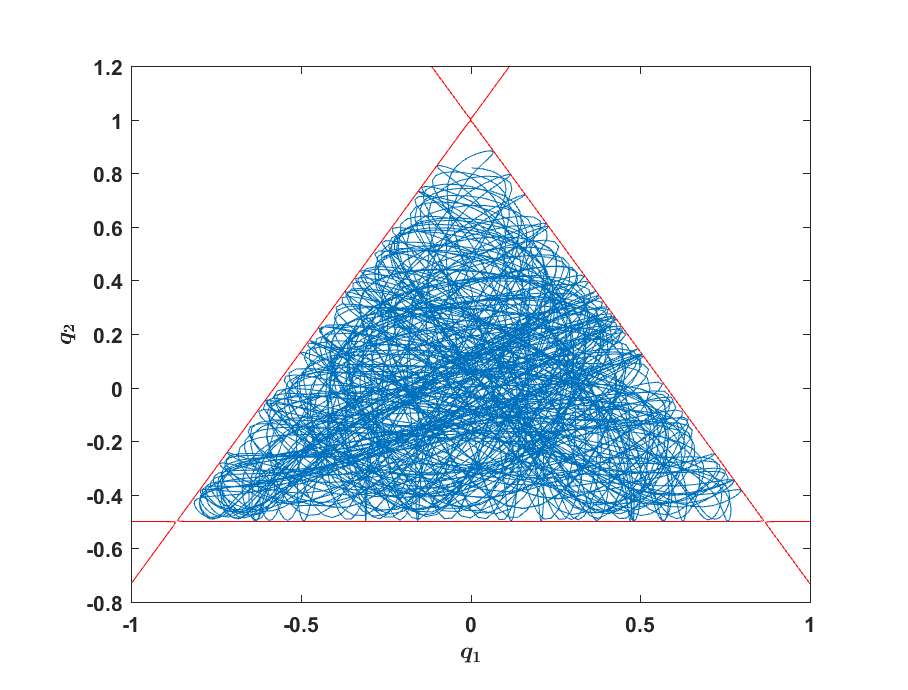
\includegraphics[width=42mm]{cHH2_R}
\end{minipage}}
\end{figure}
\end{frame}

\begin{frame}{Energy conservation of AVF, Schemes EI and EII}
\begin{figure}
\centering
\subfigure[Box orbits]{
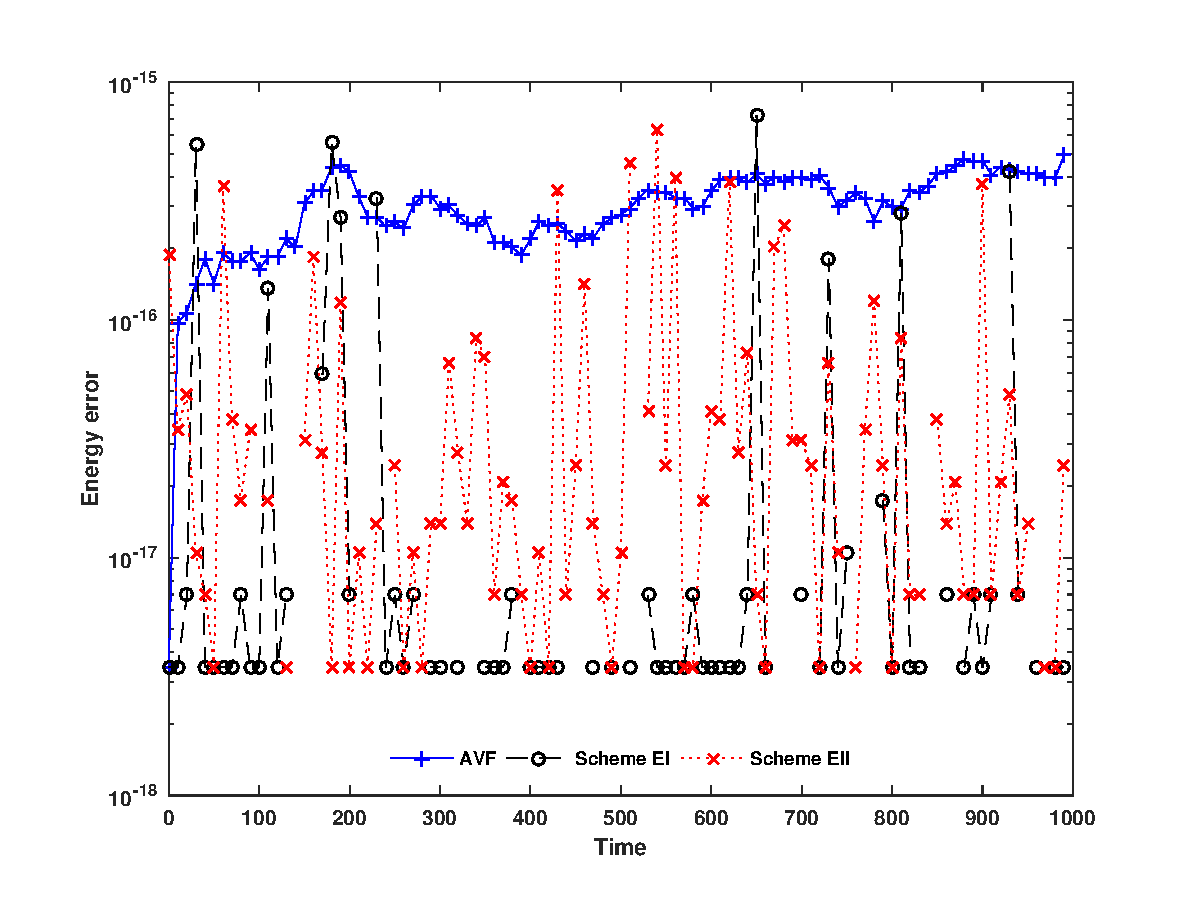
\includegraphics[width=0.33\textwidth]{bHH_EPS_HE}\hspace{-4mm}
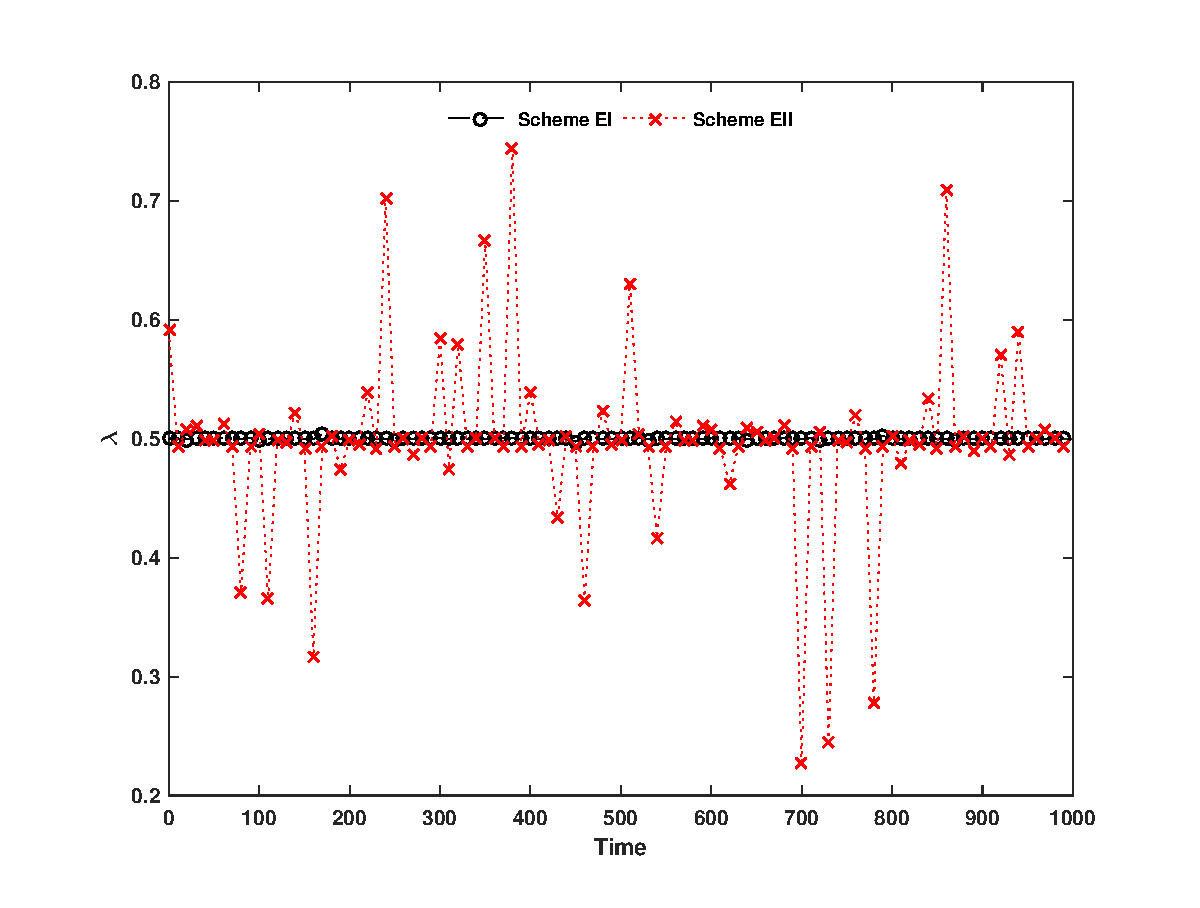
\includegraphics[width=0.33\textwidth]{bHH_par}\hspace{-4mm}
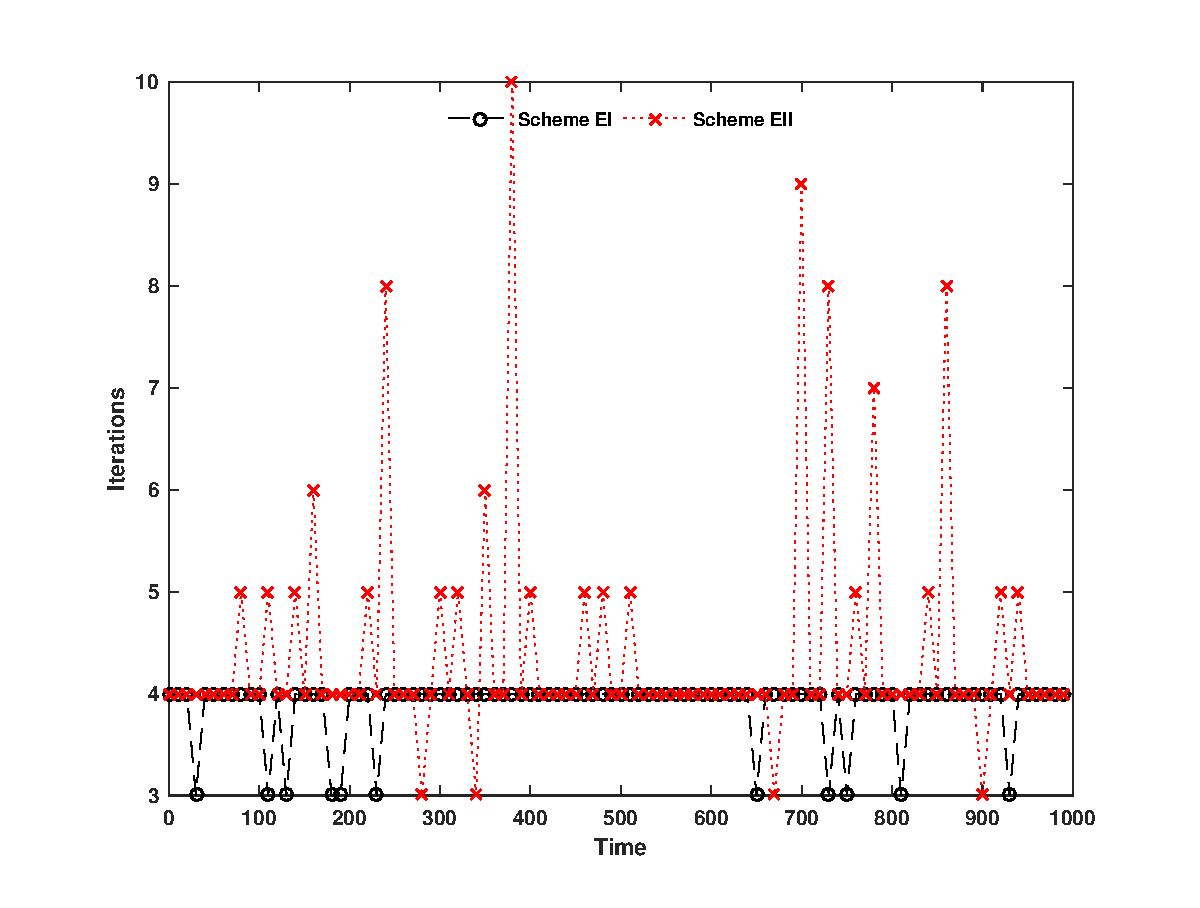
\includegraphics[width=0.33\textwidth]{bHH_Iter}}\vspace{-1mm}
\subfigure[Chaotic orbits]{
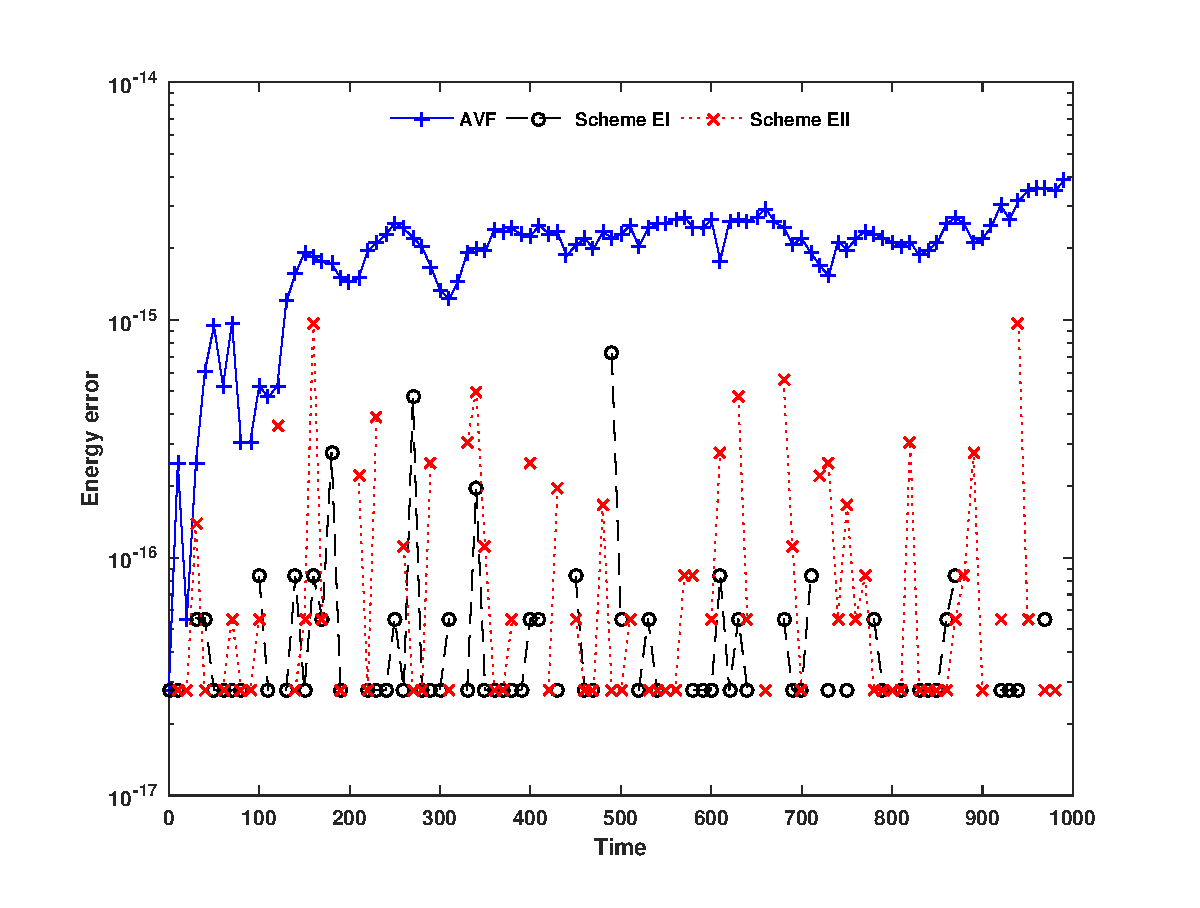
\includegraphics[width=0.33\textwidth]{cHH_EPS_HE}\hspace{-4mm}
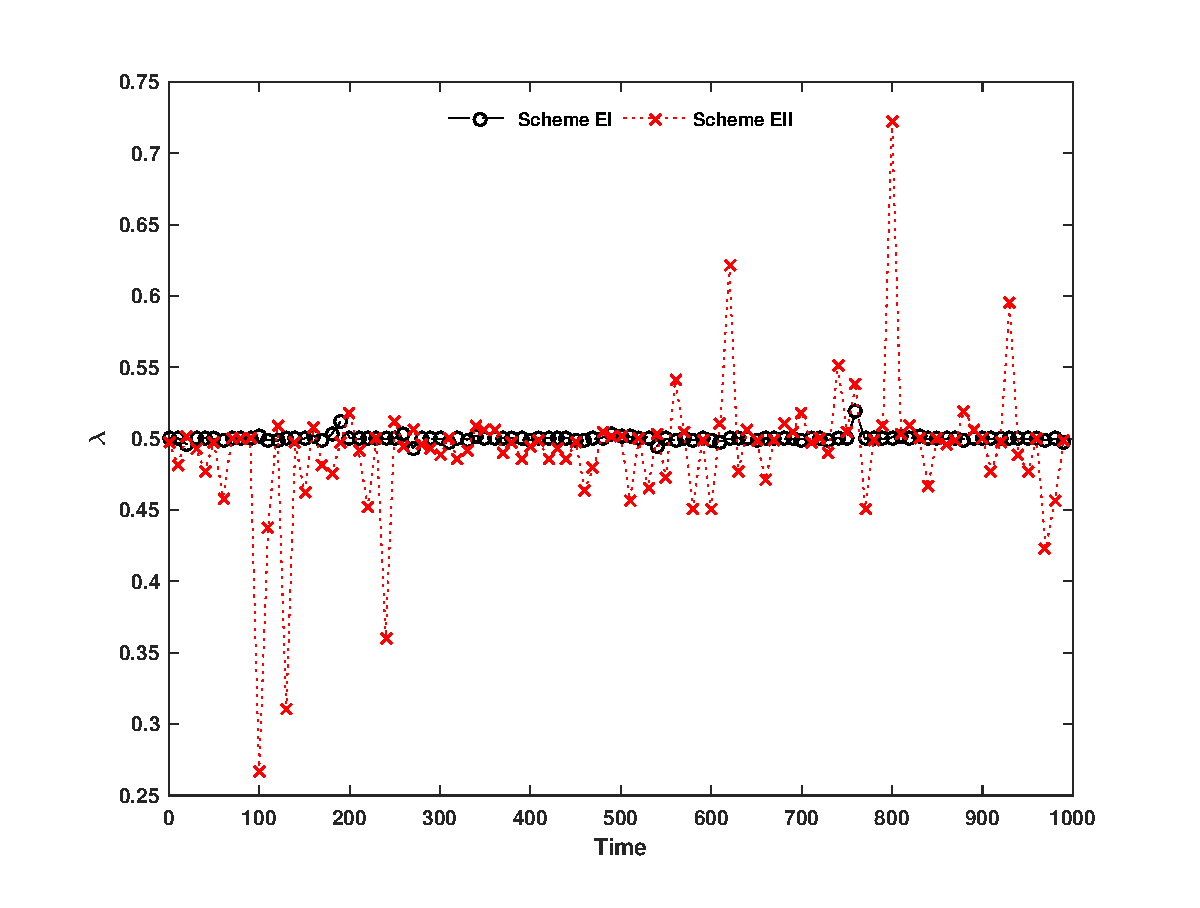
\includegraphics[width=0.33\textwidth]{cHH_par}\hspace{-4mm}
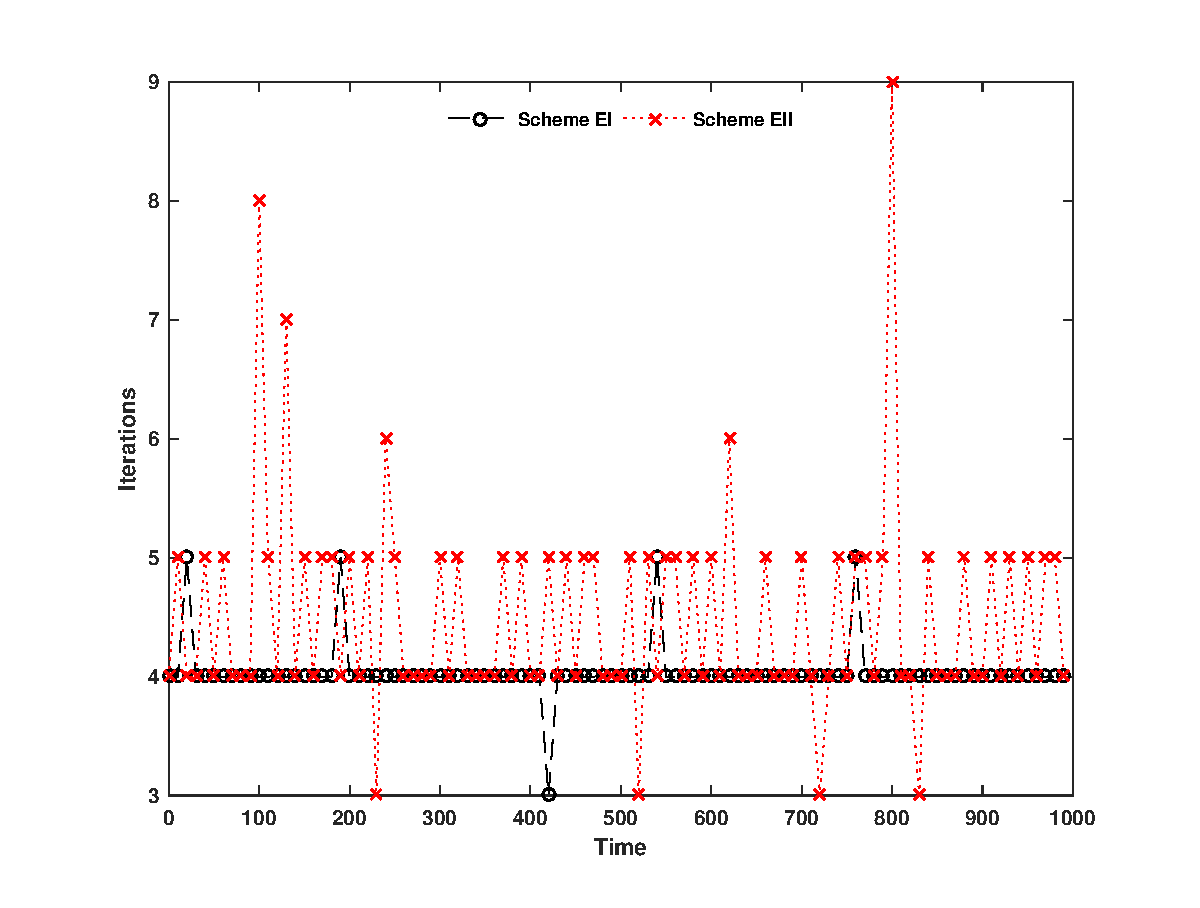
\includegraphics[width=0.33\textwidth]{cHH_Iter}}
\end{figure}
\end{frame}

\begin{frame}{Convergence tests with chaotic orbits at $t=1$}
\begin{table}[H]
\tabcolsep=10.5pt \small \renewcommand\arraystretch{1.5} \centering
\begin{tabularx}{\textwidth}{*{7}{l}} \toprule
\multirow{2}*{$\tau$} & \multicolumn{2}{c}{AVF} & \multicolumn{2}{c}{Scheme EI} & \multicolumn{2}{c}{Scheme EII}\\
\cmidrule(lr){2-3}\cmidrule(lr){4-5}\cmidrule(lr){6-7}
& Error & Order & Error & Order & Error & Order\\ \midrule
0.02/2 & 1.78E-05 & - & 2.50E-03 & - & 4.23E-06 & -\\
0.02/4 & 4.46E-06 & 2.00 & 1.24E-03 & 1.01 & 1.06E-06 & 2.00\\
0.02/8 & 1.11E-06 & 2.00 & 6.22E-04 & 0.99 & 2.64E-07 & 2.00\\
0.02/16 & 2.78E-07 & 2.00 & 3.10E-04 & 1.00 & 6.60E-08 & 2.00\\ \bottomrule
\end{tabularx}
\end{table}
\end{frame}

\begin{frame}{Numerical experiments: the perturbed Kepler problem}
\begin{figure}[H]
\centering
\subfigure[AVF]{
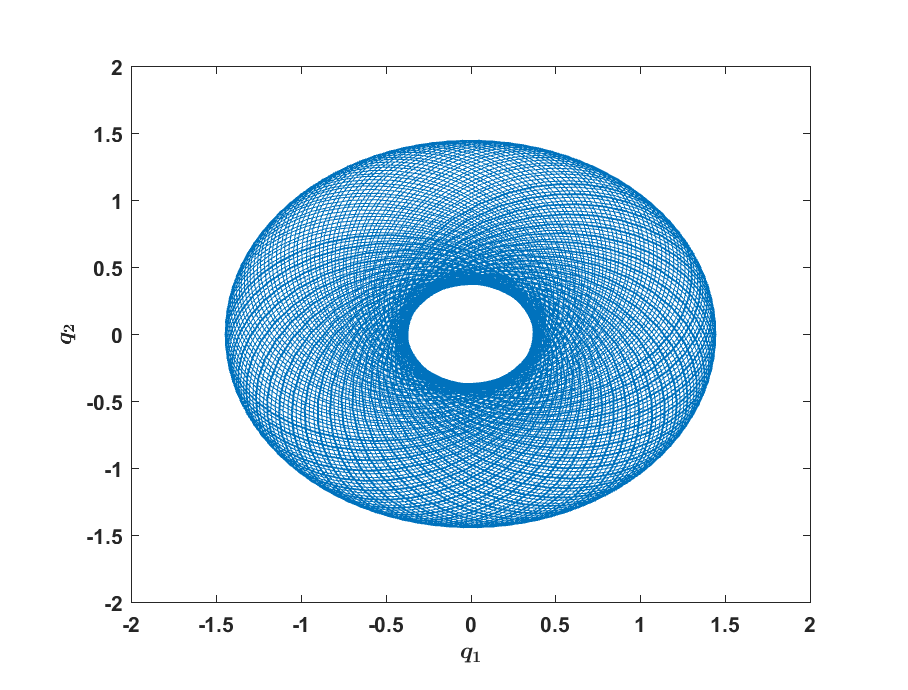
\includegraphics[width=42mm]{perkepler_AVF_R}}\vspace{-1mm}\\
\subfigure[Scheme EI]{
\includegraphics[width=42mm]{perkepler_EPS_R}}
\subfigure[Scheme EII]{
\includegraphics[width=42mm]{perkepler2_EPS_R}}
\end{figure}
\end{frame}

\begin{frame}{Energy and angular momentum conservations of AVF, Schemes EI and EII}
\begin{figure}
\centering
\subfigure[Energy conservation]{
\includegraphics[width=42mm]{perkepler_EPS_HE}}
\subfigure[Angular momentum conservation]{
\includegraphics[width=42mm]{perkepler_EPS_LE}}
\subfigure[Parameter]{
\includegraphics[width=42mm]{perkepler_EPS_par}}
\subfigure[Iterations]{
\includegraphics[width=42mm]{perkepler_EPS_Iter}}
\end{figure}
\end{frame}	

\begin{frame}{Numerical experiments: the sine-Gordon equation}
\begin{figure}
\centering
\subfigure[$T=0$]{
\includegraphics[width=0.33\textwidth]{CRS_solu_E0}}\hspace{-4mm}
\subfigure[$T=2.8$]{
\includegraphics[width=0.33\textwidth]{CRS_solu_E1}}\hspace{-4mm}
\subfigure[$T=5.6$]{
\includegraphics[width=0.33\textwidth]{CRS_solu_E2}}\vspace{-1mm}
\subfigure[$T=8.4$]{
\includegraphics[width=0.33\textwidth]{CRS_solu_E3}}\hspace{-4mm}
\subfigure[$T=11.2$]{
\includegraphics[width=0.33\textwidth]{CRS_solu_E4}}\hspace{-4mm}
\subfigure[$T=12.6$]{
\includegraphics[width=0.33\textwidth]{CRS_solu_E5}}
\end{figure}	
\end{frame}
	
\begin{frame}{Collision of four circular solitons of Scheme EI}
\begin{figure}
\centering
\subfigure[$T=0$]{
\includegraphics[width=0.33\textwidth]{CCS_solu_E0}}\hspace{-4mm}
\subfigure[$T=2.5$]{
\includegraphics[width=0.33\textwidth]{CCS_solu_E1}}\hspace{-4mm}
\subfigure[$T=5$]{
\includegraphics[width=0.33\textwidth]{CCS_solu_E2}}\vspace{-1mm}
\subfigure[$T=7.5$]{
\includegraphics[width=0.33\textwidth]{CCS_solu_E3}}\hspace{-4mm}
\subfigure[$T=10$]{
\includegraphics[width=0.33\textwidth]{CCS_solu_E4}}
\end{figure}	
\end{frame}	

\begin{frame}{Energy conservation of Scheme EI}
\begin{figure}
\centering
\subfigure[Circular ring soliton]{
\includegraphics[width=0.33\textwidth]{CRS_EPS_HE}\hspace{-4mm}
\includegraphics[width=0.33\textwidth]{CRS_EPS_par}\hspace{-4mm}
\includegraphics[width=0.33\textwidth]{CRS_EPS_Iter}}\vspace{-1mm}
\subfigure[Collision of four circular solitons]{
\includegraphics[width=0.33\textwidth]{CCS_EPS_HE}\hspace{-4mm}
\includegraphics[width=0.33\textwidth]{CCS_EPS_par}\hspace{-4mm}
\includegraphics[width=0.33\textwidth]{CCS_EPS_Iter}}
\end{figure}
\end{frame}

	
\section{Linearly implicit energy-preserving methods for Hamiltonian PDEs}
\begin{frame}{Hamiltonian PDEs}
\textcolor[rgb]{0,0,1}{$\blacktriangleright$} \textcolor{blue}{Hamiltonian PDEs:}
\begin{equation}\label{eq-29}
z_t=\mathcal{D}\frac{\delta \mathcal{H}}{\delta z},\quad \mathcal{H}(z)=\frac{1}{2}\big(z,\mathcal{L}z\big)+\big(\mathcal{N}(z),1\big),
\end{equation} 
where $\mathcal{D}$ is a skew-adjoint operator and $\mathcal{L}$ is a symmetric non-negative linear operator, $(x,t) \in \Omega\times[0,T]$ and $\Omega \in \mathcal{R}^d$.  The system \eqref{eq-29} can be rewritten as
\begin{equation}\label{eq-30}
\begin{aligned}
z_t&=\mathcal{D}\mu,\\
\mu&=\mathcal{L}z+\mathcal{N}^\prime(z).
\end{aligned}
\end{equation} 
\vspace{2mm}
\textcolor[rgb]{0,0,1}{$\blacktriangleright$} \textcolor{blue}{Existing numerical methods:}\\
\quad\textcolor[rgb]{0,0,1}{$\bullet$} Discrete gradient methods. Quispel, 1998.\\
\quad\textcolor[rgb]{0,0,1}{$\bullet$} Discrete variational derivative methods. Furihata, Matsuo, 1999.\\
\quad\textcolor[rgb]{0,0,1}{$\bullet$} Time finite element methods. Betsch, Steinmann, 2000.\\
\quad\textcolor[rgb]{0,0,1}{$\bullet$} Averaged vector field methods. Quispel, McLaren, 2008.\\
\quad\textcolor[rgb]{0,0,1}{$\bullet$} Hamiltonian boundary value methods. Brugnano, 2010.$\cdots$\\
\end{frame}

\begin{frame}{Motivations}
\quad\textcolor[rgb]{0,0,1}{$\bullet$} The conventional energy-preserving methods are fully implicit, and time-consuming nonlinear iterations cannot be avoided in programming. \\
\vspace{2mm}
\quad\textcolor[rgb]{0,0,1}{$\bullet$} One alternative way to incorporate the energy-preserving property and computational efficiency is to construct linearly implicit schemes:\\
\vspace{1mm}
\quad\quad\textcolor[rgb]{0,0,1}{-} Multiple discrete variational derivative methods. Furihata, 2001.\\
\quad\quad\textcolor[rgb]{0,0,1}{-} Polarization technique. Dahlby, Owren, 2011.\\	
\quad\quad\textcolor[rgb]{0,0,1}{-} Invariant energy quadratization method. Yang, 2016.\\
\quad\quad\textcolor[rgb]{0,0,1}{-} Scalar auxiliary variable approach. Shen, 2018.\\
\vspace{2mm}
\quad\textcolor[rgb]{0,0,1}{$\bullet$} Most of the linearly implicit energy-preserving methods are second-order accuracy, which cannot meet the high-accuracy requirement of some practical problems.\\
\vspace{2mm}
\quad\textcolor[rgb]{0,0,1}{$\bullet$} How to construct a higher-order linearly implicit energy-preserving method by selecting more stages of Gauss RK methods and higher-order extrapolations??
\end{frame}

\begin{frame}{Standard scalar auxiliary variable approach\footnote{W. Cai, C. Jiang, Y. Wang, and Y. Song. {\em J. Comput. Phys.}, 395:166–185, 2019.}}
Introducing a auxiliary variable $w(t)=\sqrt{\big(\mathcal{N}(z),1\big)+C_0}$ with the assumption that $\big(\mathcal{N}(z),1\big)$ is bounded from below, the system \eqref{eq-30} can be rewritten in the equivalent form
\begin{align}\label{eq-31}
\aligned
&z_t=\mathcal{D}\mu,\\
&\mu~=\mathcal{L}z+A(z)w,\quad A(z)=\frac{\mathcal{N}'(z)}{\sqrt{\big(\mathcal{N}(z),1\big)+C_0}},\\
&w_t=\frac{1}{2}\big(A(z),z_t\big).
\endaligned
\end{align}
The above system satisfies the modified energy conservation law
\begin{equation}\label{eq-32}
\frac{d}{dt}\mathcal{H}(t)=0,\quad\mathcal{H}(t)=\frac{1}{2}\big(z,\mathcal{L}z\big)+w^2.
\end{equation} 	
\end{frame}

\begin{frame}
\textcolor[rgb]{0,0,1}{$\blacktriangleright$} \textcolor{blue}{SAV-CN:}
\begin{align}\label{eq-33}
\aligned
&z^{n+1}-z^n=\tau\mathcal{D}\mu^{n+\frac{1}{2}},\\
&\mu^{n+\frac{1}{2}}=\mathcal{L}z^{n+\frac{1}{2}}+A(\bar{z}^{n+\frac{1}{2}})w^{n+\frac{1}{2}},\quad A(\bar{z}^{n+\frac{1}{2}})\triangleq A^n,\\
&w^{n+1}-w^n=\frac{1}{2}\big(A(\bar{z}^{n+\frac{1}{2}}),z^{n+1}-z^n\big).
\endaligned
\end{align}\\
\quad\textcolor[rgb]{0,0,1}{$\bullet$} Semi-discrete energy conservation law:
\begin{equation}\label{eq-34}
\mathcal{H}^{n+1}=\mathcal{H}^n,\quad\mathcal{H}^n=\frac{1}{2}\big(z^n,\mathcal{L}z^n\big)+(w^n)^2.
\end{equation} 
\quad\textcolor[rgb]{0,0,1}{$\bullet$} Computing implementation:
\begin{subequations}\label{eq-35}
\begin{align}
&\left(A^n,z^{n+1}\right)=\frac{\left(A^n,(\mathcal{I}-\frac{1}{2}\tau\mathcal{D}\mathcal{L})^{-1}C^n\right)}{1-\frac{1}{4}\tau\left(A^n,(\mathcal{I}-\frac{1}{2}\tau\mathcal{D}\mathcal{L})^{-1}\mathcal{D}A^n\right)},\label{eq-35-a}\\
&z^{n+1}=\left(\mathcal{I}-\frac{1}{2}\tau\mathcal{D}\mathcal{L}\right)^{-1}C^n+\frac{1}{4}\tau\left(\mathcal{I}-\frac{1}{2}\tau\mathcal{D}\mathcal{L}\right)^{-1}\mathcal{D}A^n\left(A^n,z^{n+1}\right),\label{eq-35-b}\\
&w^{n+1}=w^n+\frac{1}{2}\big(A(\bar{z}^{n+\frac{1}{2}}),z^{n+1}-z^n\big).\label{eq-35-c}
\end{align}
\end{subequations} 
\end{frame}

\begin{frame}{Exponential scalar auxiliary variable approach\footnote{Y.H. Bo, Y.S. Wang, and W.J. Cai. arXiv:2011.08375, 2020.}}
let $e(t)=\exp\big((\mathcal{N}(z),1)\big)$, the system \eqref{eq-30} can be reformulated as
\begin{align}\label{eq-36}
\aligned
&z_t=\mathcal{D}\mu,\\
&\mu~=\mathcal{L}z+B(z,e),\quad B(z,e)=\frac{\mathcal{N}'(z)e}{\exp\big((\mathcal{N}(z),1)\big)},\\
&\frac{d}{dt}\mbox{ln}(e)=\big(B(z,e),z_t\big).
\endaligned
\end{align}
The above system satisfies the modified energy conservation law
\begin{equation}\label{eq-37}
\frac{d}{dt}\mathcal{H}(t)=0,\quad\mathcal{H}(t)=\frac{1}{2}\big(z,\mathcal{L}z\big)+\mbox{ln}(e).
\end{equation}\\
\begin{equation*}
\textcolor{blue}{\mbox{No}\ \mbox{assumptions}\ \&\ \mbox{more}\ \mbox{practical}}
\end{equation*} 
\end{frame}

\begin{frame}
\textcolor[rgb]{0,0,1}{$\blacktriangleright$} \textcolor{blue}{ESAV-CN:}
\begin{align}\label{eq-38}
\aligned
&z^{n+1}-z^n=\tau\mathcal{D}\mu^{n+\frac{1}{2}},\\
&\mu^{n+\frac{1}{2}}=\mathcal{L}z^{n+\frac{1}{2}}+B(\bar{z}^{n+\frac{1}{2}},\bar{e}^{n+\frac{1}{2}}),\quad B(\bar{z}^{n+\frac{1}{2}},\bar{e}^{n+\frac{1}{2}})\triangleq B^n,\\
&\mbox{ln}(e^{n+1})-\mbox{ln}(e^n)=\big(B(\bar{z}^{n+\frac{1}{2}},\bar{e}^{n+\frac{1}{2}}),z^{n+1}-z^n\big).
\endaligned
\end{align}\\
\quad\textcolor[rgb]{0,0,1}{$\bullet$} Semi-discrete energy conservation law:
\begin{equation}\label{eq-39}
\mathcal{H}^{n+1}=\mathcal{H}^n,\quad\mathcal{H}^n=\frac{1}{2}\big(z^n,\mathcal{L}z^n\big)+\ln (e^n).
\end{equation} 
\quad\textcolor[rgb]{0,0,1}{$\bullet$} Computing implementation:
\begin{subequations}\label{eq-40}
\begin{align}
&z^{n+1}=\left(\mathcal{I}-\frac{1}{2}\tau\mathcal{D}\mathcal{L}\right)^{-1}\left[\big(\mathcal{I}+\frac{1}{2}\tau\mathcal{D}\mathcal{L}\big)z^n+\tau\mathcal{D}B^n\right],\label{eq-40-a}\\
&e^{n+1}=\mbox{exp}\left(\mbox{ln}(e^n)+(B^n,z^{n+1}-z^n)\right).\label{eq-40-b}
\end{align}
\end{subequations}  
\quad\textcolor[rgb]{0,0,1}{$\bullet$} \textcolor{blue}{Higher-order} linearly implicit energy-preserving methods??
\end{frame}

\begin{frame}
\textcolor[rgb]{0,0,1}{$\blacktriangleright$} \textcolor{blue}{ESAV-Gauss:}
Using the $s$-stage symplectic RK method in time discretization, we obtain
\begin{subequations}\label{eq-41}
\begin{align}
&z_i^n=z^n+\tau\sum_{j=1}^sa_{ij}k_j^n,\quad k_i^n=\mathcal{D}\mu_i^n,\quad \mu_i^n=\mathcal{L}z_i^n+B(z_{s,i}^n,e_{s,i}^n),\label{eq-41-a}\\
&e_i^n=\mbox{exp}\left(\mbox{ln}(e^n)+\tau\sum_{j=1}^sa_{ij}\mathcal{L}_j^n\right),\quad\mathcal{L}_i^n=\left(B(z_{s,i}^n,e_{s,i}^n),k_i^n\right),\quad i=1,2,\cdots,s,\label{eq-41-b}\\
&z^{n+1}=z^n+\tau\sum_{i=1}^sb_ik_i^n,\quad e^{n+1}=\mbox{exp}\left(\mbox{ln}(e^n)+\tau\sum_{i=1}^sb_i\mathcal{L}_i^n\right).\label{eq-41-c}
\end{align}
\end{subequations}\\
\quad\textcolor[rgb]{0,0,1}{$\bullet$} Semi-discrete energy conservation law:
\begin{equation}\label{eq-42}
\mathcal{H}_s^{n+1}=\mathcal{H}_s^n,\quad\mathcal{H}_s^n=\frac{1}{2}\big(z^n,\mathcal{L}z^n\big)+\ln (e^n).
\end{equation} 
\end{frame}

\begin{frame}
Taking $s=2$ as an interpretation for the nonlinear term $B(z_{s,i}^n,e_{s,i}^n)$:
\begin{equation}\label{eq-43}
\begin{aligned}
z_2^n(c)=&\frac{(1+c-c_1)(1+c-c_1)}{c_1c_2}z^{n-1}+\frac{(1+c)(1+c-c_2)}{c_1(c_1-c_2)}z_1^{n-1}\\
&+\frac{(1+c)(1+c-c_1)}{c_2(c_2-c_1)}z_2^{n-1}.\\
\end{aligned}
\end{equation}
with $c_1=\frac{1}{2}-\frac{\sqrt{3}}{6}$ and $c_2=\frac{1}{2}+\frac{\sqrt{3}}{6}$. Then we have the approximation of internal values as
\begin{equation}\label{eq-44}
\begin{aligned}
&z_{2,1}^n=z_2^n(c_1)=(-2\sqrt{3}+6)z^{n-1}+(-3\sqrt{3}+1)z_1^{n-1}+(5\sqrt{3}-6)z_2^{n-1},\\
&z_{2,2}^n=z_2^n(c_2)=(2\sqrt{3}+6)z^{n-1}+(-5\sqrt{3}-6)z_1^{n-1}+(3\sqrt{3}+1)z_2^{n-1}.
\end{aligned}
\end{equation}
\begin{table}[H]
\tabcolsep=18pt \small \renewcommand \arraystretch{1.3} \centering
\caption{Coefficients of the interpolation polynomial with $s=3$.}
\begin{tabularx}{\textwidth}{*{5}{c}} \toprule
$t_n+c_i\tau$ & $z^{n-1}~(e^{n-1})$ & $z_1^{n-1}~(e_1^{n-1})$ & $z_2^{n-1}~(e_2^{n-1})$  & $z_3^{n-1}~(e_3^{n-1})$ \\ \midrule
\multirow{1}*{$z_{3,1}^{n}~(e_{3,1}^{n})$}
& $6\sqrt{15}-26$ & $-5\sqrt{15}/3+11$ & $16\sqrt{15}/3-24$ & $-29\sqrt{15}/3+40$\\
\multirow{1}*{$z_{3,2}^{n}~(e_{3,2}^{n})$}
& $-17$ & $5\sqrt{15}/2+35/2$ & $-17$ & $-5\sqrt{15}/2+35/2$\\ 
\multirow{1}*{$z_{3,3}^{n}~(e_{3,3}^{n})$}
& $-6\sqrt{15}-26$ & $29\sqrt{15}/3+40$ & $-16\sqrt{15}/3-24$ & $5\sqrt{15}/3+11$\\ \bottomrule
\end{tabularx}
\end{table}	 
\end{frame}

\begin{frame}
\textcolor[rgb]{0,0,1}{$\blacktriangleright$} \textcolor{blue}{ESAV-Gauss-PC:}
Let $\lambda$ and $\Lambda$ be iteration variable and maximal iteration step, respectively. Setting $z_i^{n(1)}=z_{s,i}^n$ and $e_i^{n(1)}=e_{s,i}^n$, then we iteratively solve $z_i^{n(\lambda+1)}$ and $e_i^{n(\lambda+1)}$ from $\lambda=1,2,\cdots,\Lambda$ by
\begin{equation}\label{eq-45}
\begin{aligned}
&z_i^{n(\lambda+1)}=z^n+\tau\sum_{j=1}^sa_{ij}k_j^{n(\lambda+1)},\quad k_i^{n(\lambda+1)}=\mathcal{D}\mu_i^{n(\lambda+1)},\\
&\mu_i^{n(\lambda+1)}=\mathcal{L}z_i^{n(\lambda+1)}+B\left(z_i^{n(\lambda)},e_i^{n(\lambda)}\right),\quad\mathcal{L}_i^{n(\lambda+1)}=\left(B\left(z_i^{n(\lambda)},e_i^{n(\lambda)}\right),k_i^{n(\lambda+1)}\right),\\
&e_i^{n(\lambda+1)}=\exp\left(\ln (e_n)+\tau\sum_{j=1}^sa_{ij}\mathcal{L}_j^{n(\lambda+1)}\right),\quad i=1,2,\cdots,s.\\
\end{aligned}
\end{equation}
If $\max\limits_{1\leq i\leq s}\left\{\|z_i^{n(\lambda+1)}-z_i^{n(\lambda)}\|_{\infty},~\|e_i^{n(\lambda+1)}-e_i^{n(\lambda)}\|_{\infty}\right\}<\mbox{TOL}$, the iteration procedure is terminated with evaluating $k_i^{n(\lambda+1)}$ and $\mathcal{L}_i^{n(\lambda+1)}$. And if not, we take $k_i^{n(\lambda+1)}=k_i^{n(\Lambda+1)}$, $\mathcal{L}_i^{n(\lambda+1)}=\mathcal{L}_i^{n(\Lambda+1)}$. Finally, the numerical solutions are updated by
\end{frame}

\begin{frame}
\begin{equation}\label{eq-46}
z^{n+1}=z^n+\tau\sum_{i=1}^sb_ik_i^{n(\lambda+1)},\quad e^{n+1}=\exp\left(\ln (e^n)+\tau\sum_{i=1}^sb_i\mathcal{L}_i^{n(\lambda+1)}\right).
\end{equation}\\
\quad\textcolor[rgb]{0,0,1}{$\bullet$} Semi-discrete energy conservation law:
\begin{equation}\label{eq-47}
\mathcal{H}_s^{n+1}=\mathcal{H}_s^n,\quad\mathcal{H}_s^n=\frac{1}{2}\big(z^n,\mathcal{L}z^n\big)+\ln (e^n).
\end{equation}\\
\textcolor[rgb]{0,0,1}{$\blacktriangleright$} \textcolor{blue}{Concluding remarks:}\\
\vspace{2mm}
\quad\textcolor[rgb]{0,0,1}{$\bullet$} A novel strategy is explored to systematically construct linearly implicit energy-preserving schemes.\\
\vspace{2mm}
\quad\textcolor[rgb]{0,0,1}{$\bullet$} Such schemes can be easily generalized to arbitrary high order.\\
\vspace{2mm}
\quad\textcolor[rgb]{0,0,1}{$\bullet$} The resulting schemes are decoupled and allow explicit implementations.\\
\vspace{2mm}
\quad\textcolor[rgb]{0,0,1}{$\bullet$} When the linear terms of the Hamiltonian functional are constant, the solutions can be explicitly solved by using the fast Fourier transform.
\end{frame}

\begin{frame}{Numerical experiments: the nonlinear Schr\"odinger equation}
We investigate the nonlinear Schr\"odinger equation
\begin{equation*}
\mbox{i}u_t+\triangle u +\beta |u|^2u=0,\quad (x,y)\in\Omega\in\mathcal{R}^2,\ t\in (0,T]
\end{equation*} 
that generates a progressive plane wave solution
\begin{equation*}
u(x,y,t)=A\ \mbox{exp}\big(\mbox{i}(c_1x+c_2y-\omega t)\big)
\end{equation*} 
with $\omega=c_1^2+c_2^2-\beta A^2$. \\
\vspace{2mm}
\begin{itemize}
\item This example is numerically solved on the spatial region $\Omega=[0,2\pi)\times[0,2\pi)$, where we choose $\beta=c_1=c_2=A=1$. 
\item The exact solution gives the initial condition by setting $t=0$, and $(2\pi,2\pi)$-periodic boundary condition is used. 	
\item The spatial Fourier pseudo-spectral method is used.
\end{itemize}
\end{frame}

\begin{frame}{Convergence rates of SAV-CN and ESAV-CN in time}
\begin{table}[H]
\tabcolsep=11.5pt \small \renewcommand \arraystretch{1.3} \centering
\caption{Convergence rates of SAV-CN and ESAV-CN in time with $N=64$ at $T=1$.}
\begin{tabularx}{\textwidth}{*{7}{l}} \toprule
Schemes & $\tau$ & $0.001$ & $0.001/2$ & $0.001/4$ & $0.001/8$ & $0.001/16$\\ \midrule 
\multirow{5}*{SAV-CN}
& L$^2$ error & 3.66E-06 & 9.16E-07 & 2.29E-07 & 5.73E-08 & 1.43E-08\\
& Order & -- & 2.00 & 2.00 & 2.00 & 2.00\\
& L$^\infty$ error & 5.82E-07 & 1.46E-07 & 3.64E-08 & 9.11E-09 & 2.28E-09\\
& Order & -- & 2.00 & 2.00 & 2.00 & 2.00\\
& CPU time & 2.38s & 4.35s & 8.67s & 17.32s & 34.54s\\ \midrule
\multirow{5}*{ESAV-CN}
& L$^2$ error & 1.05E-06 & 2.62E-07 & 6.55E-08 & 1.64E-08 & 4.08E-09\\
& Order & -- & 2.00 & 2.00 & 2.00 & 2.00\\
& L$^\infty$ error & 1.67E-07 & 4.17E-08 & 1.04E-08 & 2.60E-09 & 6.50E-10\\
& Order & -- & 2.00 & 2.00 & 2.00 & 2.00\\
& CPU time & 1.53s & 2.84s & 5.16s & 10.39s & 21.50s\\ \bottomrule
\end{tabularx}
\end{table}		
\end{frame}	

\begin{frame}{Numerical error comparisons between SAV-CN and ESAV-CN until T = 1}
\begin{figure}[H]
\centering
\subfigure[L$^2$ error]{
\includegraphics[width=42mm]{NLS_AE_solu_L2_error}}
\subfigure[L$^\infty$ error]{
\includegraphics[width=42mm]{NLS_AE_solu_Linf_error}}\vspace{-1mm}\\
\subfigure[Energy errors]{
\includegraphics[width=42mm]{NLS_AE_energy_error}}
\end{figure}
\end{frame}	

\begin{frame}{Convergence rates of Gauss, ESAV-Guass and ESAV-Gauss-PC at T=1}
\begin{figure}
\centering
\subfigure[ESAV-Gauss (left)]{
\begin{minipage}[t]{0.33\textwidth}
\centering
\includegraphics[width=42mm]{NLS_AE_L2_order}\\
\includegraphics[width=42mm]{NLS_AE_Linf_order}
\end{minipage}}
\subfigure[ESAV-Gauss-PC (right)]{
\begin{minipage}[t]{0.33\textwidth}
\centering
\includegraphics[width=42mm]{NLS_AE_L2_pc_order}\\
\includegraphics[width=42mm]{NLS_AE_Linf_pc_order}
\end{minipage}}
\end{figure}
\end{frame}

\begin{frame}{Numerical experiments: the Korteweg-de Vries equation}
\begin{equation*}
u_t+\alpha u_{xxx}+\beta uu_x=0,\quad (x,y)\in\Omega\in\mathcal{R},\ t\in (0,T]
\end{equation*} 
with $\beta=1$ and periodic boundary conditions. The two different initial conditions are as follows:
\begin{itemize}
\item One-soliton wave solution: 
\begin{equation*}
\begin{aligned}
&u(x,t)= 3\gamma\bigg[\mbox{sech}\left(\sqrt{\frac{\gamma}{4\alpha}}(x-\gamma t)_\Omega\right)\bigg]^2, \\ &\Omega=[-3,5],\ \alpha=0.0013020833,\ \gamma=1/3;
\end{aligned}
\end{equation*}
\item Two-soliton waves solution: 
\begin{equation*}
\begin{aligned}
&u(x,t)=12\frac{k_1^2e^{\xi_1}+k_2^2e^{\xi_2}+2(k_2-k_1)^2e^{\xi_1+\xi_2}+\rho^2(k_2^2e^{\xi_1}+k_1^2e^{\xi_2})e^{\xi_1+\xi_2}}{\left(1+e^{\xi_1}+e^{\xi_2}+\rho^2e^{\xi_1+\xi_2}\right)^2},\\
&\Omega=[-40,40],\ \alpha=1.
\end{aligned}
\end{equation*}
\end{itemize}
\end{frame}

\begin{frame}{One-soliton wave of ESAV-CN}
\begin{figure}[H]
\centering
\includegraphics[width=0.45\linewidth]{KDV_OS_ESAV_CN}\hspace{-2mm}
\includegraphics[width=0.45\linewidth]{KDV_OS_ESAV_CN_time}
\caption{The blue line is the exact solution, and the red circle is the numerical solutions with $N=128$ and $\tau=0.01$.}
\end{figure}
\end{frame}

\begin{frame}{Two-soliton waves of ESAV-CN}
\begin{figure}[H]
\centering
\includegraphics[width=0.33\linewidth]{KDV_TS_ESAV_CN_1}\hspace{-3mm}
\includegraphics[width=0.33\linewidth]{KDV_TS_ESAV_CN_2}\hspace{-3mm}
\includegraphics[width=0.33\linewidth]{KDV_TS_ESAV_CN_3}\\
\includegraphics[width=0.33\linewidth]{KDV_TS_ESAV_CN_time1}\hspace{-3mm}
\includegraphics[width=0.33\linewidth]{KDV_TS_ESAV_CN_time2}\hspace{-3mm}
\includegraphics[width=0.33\linewidth]{KDV_TS_ESAV_CN_time3}	
\caption{The blue line is the exact solution, and the red circle is the numerical solutions with $N=128$ and $\tau=0.01$.}
\end{figure}
\end{frame}

\begin{frame}{Energy conservation of the Korteweg-de Vries equation}
\begin{figure}
\centering
\subfigure[One-soliton wave]{
\includegraphics[width=0.45\linewidth]{KDV_OS_energy}}\hspace{-2mm}
\subfigure[Two-soliton waves]{
\includegraphics[width=0.45\linewidth]{KDV_TS_energy}}
\end{figure}
\end{frame}

%\section{Linearly implicit local energy-preserving methods for Hamiltonian PDEs}
%\begin{frame}{Multi-symplectic Hamiltonian PDEs}
%\textcolor[rgb]{0,0,1}{$\blacktriangleright$} \textcolor{blue}{Multi-symplectic formulation:}
%\begin{equation}\label{eq-48}
%Mz_t+Kz_x=\nabla S(z),
%\end{equation}
%where $M$ and $K$ are two skew-symmetric matrices, $S$ is a scalar-valued smooth function, $z\in\mathcal{R}^d$, $(x,t) \in\Omega\times[0,T]$ and $\Omega \in \mathcal{R}$.\\
%\vspace{2mm}
%\textcolor[rgb]{0,0,1}{$\blacktriangleright$} \textcolor{blue}{Local energy conservation:}\\
%\begin{equation}\label{eq-49}
%\frac{\partial}{\partial t}E+\frac{\partial}{\partial x}F=0,
%\end{equation}
%where $K=K_{+}-K_{+}^T$, $E=S(z)+z_x^TK_{+}z$ and $F=-z_t^TK_{+}z$ are the energy density and fluxes, respectively. Furthermore, with appropriate boundary conditions such as periodic/homogeneous boundary conditions, we have\\
%\vspace{2mm}
%\textcolor[rgb]{0,0,1}{$\blacktriangleright$} \textcolor{blue}{Global energy conservation:}\\
%\begin{equation}\label{eq-50}
%\frac{d}{dt}\mathcal{H}(t)=0,\quad \mathcal{H}(t)=\int_{\Omega}(S(z)+z_x^TK_{+}z)dx.
%\end{equation}
%\end{frame}
%
%\begin{frame}
%\textcolor[rgb]{0,0,1}{$\blacktriangleright$} \textcolor{blue}{Existing numerical methods:}\\
%\vspace{2mm}
%\quad\textcolor[rgb]{0,0,1}{$\bullet$} Local structure-preserving algorithms. Wang, 2008.\\
%\quad\textcolor[rgb]{0,0,1}{$\bullet$} Averaged vector field methods. Gong, Cai, Wang, 2014.$\cdots$\\
%\vspace{2mm}
%\quad\textcolor[rgb]{0,0,1}{$\bullet$} Invariant energy quadratization approach. Cai, Jiang, 2019.\\
%\quad\textcolor[rgb]{0,0,1}{$\bullet$} Kahan's method, Eidnes, Li, 2020.\\
%\vspace{4mm}
%\textcolor[rgb]{0,0,1}{$\blacktriangleright$} \textcolor{blue}{Motivations:}\\
%\vspace{2mm}
%\quad\textcolor[rgb]{0,0,1}{$\bullet$} Invariant energy quadratization approach:\\
%\vspace{1mm}
%\quad\quad\textcolor[rgb]{0,0,1}{-} The solution variable and the auxiliary variable are coupled.\\
%\quad\quad\textcolor[rgb]{0,0,1}{-} The coefficient matrix of the linear equation changes at each time step.\\
%\quad\quad\textcolor[rgb]{0,0,1}{-} This approach only has second-order accuracy in time.\\
%\vspace{2mm}
%\quad\textcolor[rgb]{0,0,1}{$\bullet$} For the general form of $S(z)$, is there a more effective way to construct a higher-order linearly local energy-preserving method??
%\end{frame}
%
%\begin{frame}{Exponential invariant energy quadratization approach}
%Let $S(z)=S_1(z)+S_2(z)$ with quadratic term $S_1(z)$ and non-quadratic term $S_2(z)$, introducing a auxiliary variable 
%\begin{equation}\label{eq-51}
%r(x,t;z)=\exp\big(S_2(z)\big),
%\end{equation} 	 
%then the system \eqref{eq-49} can be rewritten in the equivalent form
%\begin{align}\label{eq-52}
%\aligned
%&Mz_t+Kz_x=\nabla S_1(z)+\frac{r}{\exp\big(S_2(z)\big)}\nabla S_2(z),\\
%&\frac{d}{dt}\ln(r)=\frac{r}{\exp\big(S_2(z)\big)}z_t^T\nabla S_2(z).
%\endaligned
%\end{align}
%The above system satisfies the local energy conservation law
%\begin{equation}\label{eq-53}
%\frac{\partial}{\partial t}E+\frac{\partial}{\partial x}F=0,
%\end{equation} 	
%where $E=S_1(z)+\ln(r)+z_x^TK_{+}z$ and $F=-z_t^TK_{=}z$.
%\end{frame}
%
%\begin{frame}{Linearly implicit local energy-preserving method}
%Applying the implicit midpoint scheme in space and the Crank-Nicolson discretization in time obtains a local energy-preserving method
%\begin{align}\label{eq-54}
%\aligned
%&M\delta_tA_xz_j^n+K\delta_xA_tz_j^n=\overline{\nabla}_zS_1(A_xz_j^n,A_xz_j^{n+1})+\frac{A_x\widetilde{r}_j^{n+\frac{1}{2}}}{\exp\big(S_2(\widetilde{z}_j^{n+\frac{1}{2}})\big)}\nabla_z S_2(A_x\widetilde{z}_j^{n+\frac{1}{2}}),\\
%&\delta_tA_x\ln(r_j^n)=\frac{A_x\widetilde{r}_j^{n+\frac{1}{2}}}{\exp\big(S_2(\widetilde{z}_j^{n+\frac{1}{2}})\big)}\big(\delta_tA_xz_j^n\big)^T\nabla_z S_2(A_x\widetilde{z}_j^{n+\frac{1}{2}}),
%\endaligned
%\end{align}
%where $\delta_t z_j^n=\frac{z_j^{n+1}-z_j^n}{\tau}$, $A_xz_j^n=\frac{z_j^n+z_{j+1}^n}{2}$ and $\widetilde{z}_j^{n+\frac{1}{2}}=\frac{3z_j^n-z_j^{n-1}}{2}$.\\
%\vspace{2mm}
%\quad\textcolor[rgb]{0,0,1}{$\bullet$} Discrete local energy conservation law:
%\begin{equation}\label{eq-55}
%\delta_t E_{j+\frac{1}{2}}^n+\delta_x F_j^{n+\frac{1}{2}}=0,
%\end{equation} 	
%\end{frame}
%
%\begin{frame}
%where
%\begin{align}\label{eq-56}
%\aligned
%&E_{j+\frac{1}{2}}^n=S_1(A_xz_j^n)+A_x\ln(r_j^n)+\big(\delta_x z_j^n\big)^TK_{+}(A_x z_j^n),\\ &F_j^{n+\frac{1}{2}}=\big(\delta_t z_j^n\big)^TK_{+}(A_t z_j^n).
%\endaligned
%\end{align}\\
%\vspace{4mm}
%For the periodic/homogeneous boundary conditions, the scheme \eqref{eq-54} possesses the discrete global energy conservation law
%\begin{equation}\label{eq-57}
%\mathcal{H}^{n+1}=\mathcal{H}^{n},
%\end{equation} 	
%where
%\begin{equation}\label{eq-58}
%\mathcal{H}^{n}=h\sum_{j=0}^{N-1}E_{j+\frac{1}{2}}^n
%\end{equation} 	
%with $h$ as the step size of the space division.
%\end{frame}
%
%\begin{frame}{Numerical experiment: the Korteweg-de Vries equation}
%\begin{equation*}
%u_t+\eta uu_x+\mu^2u_{xxx}=0,
%\end{equation*} 	
%where $\eta$ and $\mu$ are two real parameters. By the covariant Legendre transform, we derive the system
%\begin{equation*}
%Mz_t+Kz_x=\nabla S(z),
%\end{equation*}
%where
%\begin{equation*}
%z=\left(\begin{array}{c} \phi\\u\\v\\w\end{array}\right),\ M=\left(\begin{array}{cccc} 0 & \frac{1}{2} & 0& 0\\ -\frac{1}{2} & 0 & 0 &0\\ 0 & 0 & 0 &0\\ 0 & 0 & 0 &0\end{array}\right),\ K=\left(\begin{array}{cccc} 0 & 0 & 0& 1\\ 0 & 0 & -\mu &0\\ 0 & \mu & 0 &0\\ -1 & 0 & 0 &0\end{array}\right)
%\end{equation*}	
%and $S(z)=\frac{1}{2}v^2-uw+\frac{\eta}{6}u^3$. The corresponding local energy conservation law is
%\begin{equation*}
%\frac{\partial}{\partial t}\left(-\frac{1}{2}v^2+\frac{\eta}{6}u^3\right)+\frac{\partial}{\partial x}\left(-w\phi_t+\mu vu_t\right)=0.
%\end{equation*}
%\end{frame}
%
%\begin{frame}
%\begin{align*}
%\aligned
%&\frac{1}{2}\delta_tA_xu_j^n+\delta_xA_tw_j^n=0,\\
%&-\frac{1}{2}\delta_tA_x\phi_j^n-\mu\delta_xA_tv_j^n=-A_tA_xw_j^n+\frac{A_x\widetilde{r}_j^{n+\frac{1}{2}}}{\exp\big(S_2(\widetilde{u}_j^{n+\frac{1}{2}})\big)}\nabla_z S_2(A_x\widetilde{z}_j^{n+\frac{1}{2}}),\\
%&\mu\delta_xA_tu_j^n=A_tA_xv_j^n,\quad\delta_xA_t\phi_j^n=A_tA_xu_j^n,\\
%&\delta_tA_x\ln(r_j^n)=\frac{A_x\widetilde{r}_j^{n+\frac{1}{2}}}{\exp\big(S_2(\widetilde{z}_j^{n+\frac{1}{2}})\big)}\big(\delta_tA_xz_j^n\big)^T\nabla_z S_2(A_x\widetilde{z}_j^{n+\frac{1}{2}}).
%\endaligned
%\end{align*}\\
%By eliminating the auxiliary variables $\phi$, $v$ and $w$, we obtain
%\begin{equation*}
%\delta_tA_x^3u_j^n+\mu^2\delta_x^3A_tu_j^n+\delta_xA_xC_j^n=0,
%\end{equation*}
%i.e.,
%\begin{equation*}
%\left(A_x^3+\frac{\tau\mu^2}{2}\delta_x^3\right)u_j^{n+1}=\left(A_x^3-\frac{\tau\mu^2}{2}\delta_x^3\right)u_j^n-\tau\delta_xA_xC_j^n.
%\end{equation*}
%\vspace{1mm}
%\begin{equation*}
%\textcolor{blue}{\mbox{Constant circulant matrix \& fast Fourier transform}}
%\end{equation*}
%\end{frame}
%
%\begin{frame}{One-soliton wave}
%\begin{figure}[H]
%\centering
%\includegraphics[width=0.45\linewidth]{KDV_OS_EIEQ}\hspace{-2mm}
%\includegraphics[width=0.45\linewidth]{KDV_OS_EIEQ_time}
%\caption{The blue line is the exact solution, and the red circle is the numerical solutions with $h=\tau=0.02$.}
%\end{figure}
%\end{frame}
%
%\begin{frame}{Two-soliton waves}
%\begin{figure}[H]
%\centering
%\includegraphics[width=0.33\linewidth]{KDV_TS_EIEQ_1}\hspace{-3mm}
%\includegraphics[width=0.33\linewidth]{KDV_TS_EIEQ_2}\hspace{-3mm}
%\includegraphics[width=0.33\linewidth]{KDV_TS_EIEQ_3}\\
%\includegraphics[width=0.33\linewidth]{KDV_TS_EIEQ_time1}\hspace{-3mm}
%\includegraphics[width=0.33\linewidth]{KDV_TS_EIEQ_time2}\hspace{-3mm}
%\includegraphics[width=0.33\linewidth]{KDV_TS_EIEQ_time3}	
%\caption{The blue line is the exact solution, and the red circle is the numerical solutions with $h=\tau=0.02$.}
%\end{figure}
%\end{frame}
%
%\begin{frame}{Local energy conservation of the Korteweg-de Vries equation}
%\begin{figure}
%\centering
%\subfigure[One-soliton wave (left)]{
%\begin{minipage}[t]{0.33\textwidth}
%\centering
%\includegraphics[width=42mm]{KDV_OS_EIEQ_Loc}\\
%\includegraphics[width=42mm]{KDV_OS_EIEQ_Glo}
%\end{minipage}}
%\subfigure[Two-soliton waves (right)]{
%\begin{minipage}[t]{0.33\textwidth}
%\centering
%\includegraphics[width=42mm]{KDV_TS_EIEQ_Loc}\\
%\includegraphics[width=42mm]{KDV_TS_EIEQ_Glo}
%\end{minipage}}
%\end{figure}
%\end{frame}

\section*{}
\begin{frame}
\begin{center}
\color{blue}\Huge Thanks for your attention!
\end{center}
\end{frame}
\end{document}
